%&../preamble

\def\npart {IB}
\def\nterm {Lent}
\def\nyear {2022}
\def\nlecturer {Prof. G. Paternain}
\def\ncourse {Geometry}

\def\encodingdefault{TU}\normalfont
\ifnum 0\ifxetex 1\fi\ifluatex 1\fi=0 % if pdftex
  \usepackage[T1]{fontenc}
  \usepackage[utf8]{inputenc}
  \usepackage{textcomp} % provide euro and other symbols
\else % if luatex or xetex
  % \usepackage{unicode-math}
  % \defaultfontfeatures{Scale=MatchLowercase}
  % \defaultfontfeatures[\rmfamily]{Ligatures=TeX,Scale=1}
  % \DeclareMathAlphabet{\mathcal}{OMS}{cmsy}{m}{n}
  % \let\mathbb\relax % remove the definition by unicode-math
  % \DeclareMathAlphabet{\mathbb}{U}{msb}{m}{n}
\fi

\usetikzlibrary{external}
\tikzset{external/system call={xelatex -fmt=../preamble.fmt \tikzexternalcheckshellescape -halt-on-error -interaction=batchmode -jobname "\image" "\texsource"}} % path is relative to file that includes preamble
\tikzexternalize

\providetoggle{DontSetTitleAuthorDate}

\nottoggle{DontSetTitleAuthorDate}{
  \hypersetup{
    pdftitle={Part \npart\ - \ncourse},
    pdfsubject={Cambridge Maths Notes: Part \npart\ - \ncourse},
    pdfkeywords={Cambridge Mathematics Maths Math \npart\ \nterm\ \nyear\ \ncourse}
  }

  \author{Based on lectures by \nlecturer}
  \date{\nterm\ \nyear}
  \title{Part \npart\ --- \ncourse}
}{}

\tikzsetexternalprefix{figtemp/}
\author{Based on lectures by \nlecturer \ and notes by thirdsgames.co.uk}

\usepackage{faktor}
\usepackage{scalerel}

\newcommand{\connect}{\mathbin{\#}}
\DeclareMathOperator*{\bigconnect}{\scalerel*{\#}{\textstyle\sum}}
\DeclareMathOperator{\id}{id}
\DeclareMathOperator{\Aut}{Aut}
\DeclareMathOperator{\Hom}{Hom}
\newcommand{\tran}{\intercal}
\DeclareMathOperator{\vecspan}{span}
\newcommand{\wildcard}{{}\cdot{}}
\DeclareMathOperator{\Iff}{\mathrm{I}}
\DeclareMathOperator{\IIff}{\mathrm{I\!I}}
\newcommand{\Mob}{\text{M\"ob}}
\DeclareMathOperator{\artanh}{artanh}
\newcommand{\genset}[1]{\left\langle{} #1 \right\rangle}
\newcommand{\Chat}{\widehat{\mathbb C}}
\newcommand{\acts}{\curvearrowright}

\let\emptyset\varnothing

\usepackage{../quiver}
\usepackage{../tikzit}
\input{../style.tikzstyles}

\begin{document}
    \maketitle
    \tableofcontents

    \section{Surfaces}

\subsection{Basic definitions}
\begin{definition}
	A \vocab{topological surface} is a topological space $\Sigma$ such that
	\begin{enumerate}
		\item for all points $p \in \Sigma$, there exists an open neighbourhood $p \in U \subset \Sigma$ such that $U$ is homeomorphic to $\mathbb R^2$, or a disc $D^2 \subset \mathbb R^2$, with its usual Euclidean topology;
		\item $\Sigma$ is Hausdorff and second countable.
	\end{enumerate}
\end{definition}

\begin{definition}[Hausdorff]
	A space $X$ is \vocab{Hausdorff} if two points $p \neq q \in X$ have open neighbourhoods $U, V$ such that $U \cap V = \emptyset$.
\end{definition} 

\begin{definition}[Second Countable]
	A space $X$ is \vocab{second countable} if it has a countable base; there exists a countable family of open sets $U_i$, such that every open set is a union of some of the $U_i$.
\end{definition} 

\begin{remark} \
	\begin{enumerate}
		\item $\mathbb R^2$ is homeomorphic to the open disc $D(0,1) = \qty{ x \in \mathbb R^2 : \norm{x} < 1 }$.
		\item The first part of the definition is important whilst the second part (Hausdorff and second countable) is a technical point. 
		These topological requirements are typically not the purpose of considering topological spaces, but they are occasionally technical requirements to prove interesting theorems.
		\item 	Note that subspaces of Hausdorff and second countable spaces are also Hausdorff and second countable.	
		In particular, Euclidean space $\mathbb R^n$ is Hausdorff (as $\mathbb R^n$ is a metric space) and second countable (consider the set of balls $D(p,q)$ for points $p$ with rational coordinates, and rational radii $q$).
		Hence, any subspace of $\mathbb R^n$ is implicitly Hausdorff and second countable.
	\end{enumerate} 
\end{remark}

\begin{example}
	$\mathbb R^2$ is a topological surface.
	Any open subset of $\mathbb R^2$ is also a topological surface.
	For example, $\mathbb R^2 \setminus \qty{0}$ and $\mathbb R^2 \setminus \qty{(0,0)} \cup \qty{\qty(0, \frac{1}{n}) : n = 1, 2, \dots}$ are topological surfaces.
\end{example}

\begin{example}
	Let $f : \mathbb R^2 \to \mathbb R$ be a continuous function.
	The graph of $f$, denoted $\Gamma_f$, is defined by
	\begin{align*}
		\Gamma_f = \qty{(x,y,f(x,y)) : (x,y) \in \mathbb R^2} \subset \mathbb{R}^3
	\end{align*}
	with the subspace topology when embedded in $\mathbb R^3$.

	Recall that the product topology on $X \times Y$ for $X, Y$ topological spaces, has basic open sets $U \times V$, where $U \subset X$, $V \subset Y$ open.
	Also the product topology has the feature that $g : Z \to X \times Y$ is continuous iff $\pi_x \circ g : Z \to X$ and $\pi_y \circ f : Z \to Y$ are continuous\footnote{$\pi_x, \pi_y$ are the canonical projections, $\pi_x : X \times Y \to X$}.

	Hence, any graph $\Gamma \subset X \times Y$ is homeomorphic to $X$ if $f$ is continuous.
	Indeed, the projection $\pi_x$ projects each point in the graph onto the domain.
	The function $s : x \mapsto (x,f(x))$ is continuous as $\pi_x \circ s$ and $\pi_y \circ s$ are.
	So $\pi_x \mid_{\Gamma_f}$ and $s$ are inverse homeomorphisms.

	So, in our case, the graph $\Gamma_f$ is homeomorphic to $\mathbb R^2$, and so is a topological surface.
\end{example}

\begin{remark}
	As a topological surface, $\Gamma_f$ is independent of the function $f$.
	However, we will later introduce more ways to describe topological spaces that will ascribe new properties to $\Gamma_f$ which do depend on $f$.
\end{remark}

\begin{example}
	The sphere:
	\begin{align*}
		S^2 = \qty{(x,y,z) \in \mathbb R^3 : x^2 + y^2 + z^2 = 1}
	\end{align*}
	is a topological surface, when using the subspace topology in $\mathbb R^3$.

	This is a subspace of $\mathbb{R}^3$ so is Hausdorff and second countable.
	
	Consider the stereographic projection of $S^2$ onto $\mathbb R^2$ from the north pole $(0,0,1)$.
	The projection satisfies $\pi_+ : S^2 \setminus \qty{(0,0,1)}$ and
	\begin{align*}
		(x,y,z) \mapsto \qty(\frac{x}{1-z}, \frac{y}{1-z}).
	\end{align*}
	Certainly, $\pi_+$ is continuous, since we do not consider the point $(0,0,1)$ to be in its domain.
	The inverse map is given by
	\begin{align*}
		(u,v) \mapsto \qty(\frac{2u}{u^2+v^2+1}, \frac{2v}{u^2+v^2+1}, \frac{u^2+v^2-1}{u^2+v^2+1}).
	\end{align*}
	This is also a continuous function.
	Hence $\pi_+$ is a homeomorphism.

	Similarly, we can construct the stereographic projection from the south pole, $\pi_-: S^2 \setminus \qty{(0,0,-1)} \to \mathbb{R}^2$.
	\begin{align*}
		(x,y,z) \mapsto \qty(\frac{x}{1+z}, \frac{y}{1+z}).
	\end{align*}
	This is a homeomorphism.

	Hence, every point in $S^2$ lies either in the domain of $\pi_+$ or $\pi_-$, and hence sits in an open set $S^2 \setminus \qty{(0,0,1)}$ or $S^2 \setminus \qty{(0,0,-1)}$ which are homeomorphic to $\mathbb R^2$.
	So $S^2$ is a topological surface.
\end{example}

\begin{remark}
	$S^2$ is compact by the Heine-Borel theorem; it is a closed bounded set in $\mathbb R^3$.
\end{remark}

\begin{example}
	The real projective plane is a topological surface.

	The group $\mathbb Z_2$ acts on $S^2$ by homeomorphisms via the \textit{antipodal map} $a : S^2 \to S^2$, mapping $x \mapsto -x$.
	So $\mathbb{Z}_2$ sits in the group of homeomorphisms of $S^2$, $\mathrm{Homeo}(S^2)$, as we can map $-1 \to a$.

	\begin{definition}[The Real Projective Plane]
		The real projective plane, $\mathbb{R} \mathbb{P}^2$, is the quotient of $S^2$ given by identifying every point $x$ with its image $-x$ under $a$.
		\begin{align*}
			\mathbb R \mathbb P^2 = \faktor{S^2}{\mathbb Z_2} = \faktor{S^2}{\sim};\quad x \sim a(x)
		\end{align*}
	\end{definition} 

	\begin{lemma}
		As a set, $\mathbb R \mathbb P^2$ naturally bijects with the set of straight lines in $\mathbb R^3$ through the origin.
	\end{lemma}

	\begin{proof}
		Any line through the origin intersects $S^2$ exactly in a pair of antipodal points $x, -x$.
		Similarly, pairs of antipodal points uniquely define a line through the origin.
	\end{proof}
	
	\begin{lemma}
		$\mathbb R \mathbb P^2$ is a topological surface with the \underline{quotient topology}.
	\end{lemma}

	Recall: Quotient topology : $q : X \to Y$ ($q$ the quotient map), $V \subset Y$ is open iff $q\inv V \subset X$ is open in $X$(i.e. iff $q$ is continuous).
	
	\begin{proof}
		We must check that $\mathbb R \mathbb P^2$ is Hausdorff since it is constructed by a quotient, not a subspace. \\
		If $[p] \neq [m] \in \mathbb R \mathbb P^2$, then $\pm p, \pm m \in S^2$ are distinct antipodal pairs.
		We can therefore construct distinct open discs\footnote{Just take a ball in $\mathbb{R}^3$ and intersect with $S^2$} around $p, m$ in $S^2$, and their antipodal images.
		These uniquely define open neighbourhoods of $[p], [q]$, which are disjoint, as for $q : S^2 \to \mathbb{R} \mathbb{P}^2$, $q(B_\delta(p))$ is \underline{open} since $q\inv(q(B_\delta(p))) = B_\delta(p) \cup (-B_\delta(p))$ is open.

		Similarly, we can check that $\mathbb R \mathbb P^2$ is second countable. \\
		We know that $S^2$ is second countable, so let $\mathcal U_0$ be a countable base for the topology on $S^2$.
		Let $\overline{\mathcal U_0} = \{q(u) : u \in \mathcal{U}_0\}$.
		$q(u)$ is open as $q\inv(q(u)) = u \cup (-u)$ is open. 
		$\overline{\mathcal U_0}$ is clearly countable since $\mathcal{U}_0$ is.
		Now, if $V \subset \mathbb R \mathbb P^2$ is open, then by definition of quotient topology $q^{-1}(V)$ is open in $S^2$ hence $q^{-1}(V) = \cup_\alpha U_\alpha, U_\alpha \in \mathcal{U}_0$.
		$V = q(q\inv V) = q(\cup_\alpha U_\alpha) = \cup_\alpha q(U_\alpha), q(U_\alpha) \in \overline{\mathcal{U}_0}$.

		Finally, let $p \in S^2$ and $[p] \in \mathbb R \mathbb P^2$ its image.
		Let $\overline D$ be a small (contained in an open hemisphere) closed disc, which is a neighbourhood of $p \in S^2$.
		The quotient map restricted to $\overline D$, written $\eval{q}_{\overline D} : \overline D \to q(\overline D) \subset \mathbb R \mathbb P^2$, is a continuous function from a \underline{compact} space to a \underline{Hausdorff} space.
		Further, $q$ is \underline{injective} on $\overline D$ since the disc was contained entirely in a single hemisphere so it cannot contain antipodal points. \\
		Recall from AT that the ``topological inverse function theorem" (TIFT) states that a continuous bijection from a compact space to a Hausdorff space is a \underline{homeomorphism}.\footnote{A brief proof is we want to show the inverse function is continuous, so it maps closed sets to closed sets. Take a closed set inside compact space so its compact, apply the continuous function to it so the image is compact. A compact set in a Hausdorff space is closed.} \\
		So $\eval{q}_{\overline D}$ is a homeomorphism from $\overline D$ to $q(\overline D)$.
		This then induces the homeomorphism $\eval{q}_{D} : D \to q(D)$ where $D$ is an open disc, the interior of $\overline D$.
		So by construction, $[p] \in q(D)$ has an open neighbourhood in $\mathbb R \mathbb P^2$ which is homeomorphic to an open disc on $S^2$ and so to $\mathbb{R}^2$, concluding the proof.
	\end{proof}
\end{example}
\begin{example}
	Let $S^1 = \{z \in \mathbb{C} : |z| = 1\}$ be the unit circle in $\mathbb C$, and then we define the torus to be the product space $S^1 \times S^1$, with the subspace topology from $\mathbb C^2$ (which is identical to the product topology).
	\begin{lemma}
		The torus is a topological surface.
	\end{lemma}
	\begin{proof}
		Consider the map $e : \mathbb R^2 \to S^1 \times S^1 \subset \mathbb{C} \times \mathbb{C}$ defined by
		\begin{align*}
			(s,t) \mapsto \qty(e^{2\pi i s}, e^{2 \pi i t})
		\end{align*}
		We have an equivalence relation on $\mathbb{R}^2$ given by translations by $\mathbb{Z}^2$ as $e$ is constant under them.
		This induces a map $\hat e$ from $\faktor{\mathbb R^2}{\mathbb Z^2}$.

		% https://tikzcd.yichuanshen.de/#N4Igdg9gJgpgziAXAbVABwnAlgFyxMJZABgBpiBdUkANwEMAbAVxiRAB12BbOnACwBGAgAQAlAHoAmEAF9S6TLnyEUARnJVajFmwDK41cM54u8YftWz5IDNjwEiZVZvrNWiDuwBmAJzoBjYE4efiExKRkg7l5BEQAtCNlNGCgAc3giUF8ILiQyEBwIJElqVx0PAEcQagY6ARgGAAVFexUQHyxUvhwrLJ8cvOpCpHUtNzZWOT6BxBKCosRRsvdPPl5hSYoZIA
		% Don't render this if we're hiding proofs anyway.
		\begin{center}
			\ifdefined\hideproofs
			\else
			\begin{tikzcd}
				\mathbb R^2 \arrow[d, "q"'] \arrow[r, "e"]             & S^1 \times S^1 \\
				\faktor{\mathbb R^2}{\mathbb Z^2} \arrow[ru, "\hat e"] &
			\end{tikzcd}
			\fi
		\end{center}

		Under the quotient topology given by the quotient map $q$, $\faktor{\mathbb R^2}{\mathbb Z^2}$ is a topological space.
		The map $[0,1]^2 \to \mathbb R^2 \to \faktor{\mathbb R^2}{\mathbb Z^2}$ is surjective, so $\faktor{\mathbb R^2}{\mathbb Z^2}$ is compact.
		As $e$ is constant on an equivalence class, $\hat e$ is a continuous map from a compact space to a Hausdorff space, and $\hat e$ is bijective, so $\hat e$ is a homeomorphism by TIFT.

		We already have that $S^1 \times S^1$ is compact and Hausdorff (as a closed and bounded set in $\mathbb C^2$, equivalent to $\mathbb{R}^4$), so it suffices to show it is locally homeomorphic to $\mathbb R^2$.

		Similarly to the case of $S^2 \to \mathbb{R} \mathbb{P}^2$, pick $[p] \in q(p), p \in \mathbb{R}^2$, then we can choose a small closed disc $\overline D(p) \subset \mathbb{R}^2$ such that $\overline D(p) \cap \qty(\overline D(p) + (n,m)) = \varnothing$ for all nonzero $(n,m) \in \mathbb Z^2$.
		Hence $\eval{e}_{\overline D(p)}$ and $\eval{q}_{\overline D(p)}$ are injective.
		Now, restricting to the open disc as before, we can find an open disc neighbourhood of $[p] \in \faktor{\mathbb R^2}{\mathbb Z^2}$.
		Since $[p]$ was chosen arbitrarily, $S^1 \times S^1$ is a topological surface.
	\end{proof}

	Another viewpoint: \\
	$\faktor{\mathbb R^2}{\mathbb Z^2}$ is also given by imposing on $[0, 1]^2$ the equivalence  relation
	\begin{align*}
		(x, 0) &\sim (x, 1) \quad \forall \; 0 \leq x \leq 1\\
		(0, y) &\sim (1, y) \quad \forall \; 0 \leq y \leq 1.
	\end{align*} 
\end{example}

\begin{example}
	Let $P$ be a planar Euclidean polygon (including interior), with oriented edges.
	We will pair the edges, and without loss of generality we will assume that paired edges have the same Euclidean length.
	\begin{center}
		\tikzfig{torus_polygon}
		\quad
		\tikzfig{other_square_polygon}
		\quad
		\tikzfig{hexagon}
	\end{center}
	We can assign letter names to each edge pair, and denote a polygon by the sequence of edges found when traversing in a clockwise orientation.
	The edge pair name is inverted if the edge is traversed in the reverse direction.
	Note the difference between the annotations on the first two shapes above, due to the reversed direction of the edge.

	If two edges $\{e, \hat e\}$ are paired, this defines a unique Euclidean isometry from $e$ to $\hat e$ respecting the orientation, which will be written $f_{e\hat e} : e \to \hat e$. \\
	The set of all such functions generate an equivalence relation on the polygon $P$, where we identify $x \in \partial P$ (a point on the boundary) with $f_{e \hat{e}}(x)$ whenever $x \in e$.

	\begin{lemma}
		$\faktor{P}{\sim}$, with the quotient topology, is a topological surface.
	\end{lemma}
\end{example}

\begin{example}
	Consider the torus, defined here as $T^2 = \faktor{[0,1]^2}{\sim}$.
	\begin{center}
		\tikzfig{torus_polygon}
	\end{center}
	Let $P$ be the polygon $[0,1]^2$.

	If $p$ is in the interior of $P$, then we pick $\delta > 0$ small s.t. $\overline{B_{\delta}(p)}$\footnote{The closure of $B_\delta(p)$} lies in the interior of $P$.
	Arguing as before in $\mathbb{R} \mathbb{P}^2$, the quotient map is injective on $\overline{B_{\delta}(p)}$ and is a homeomorphism on its interior.
	{ 	\par
		\centering 
		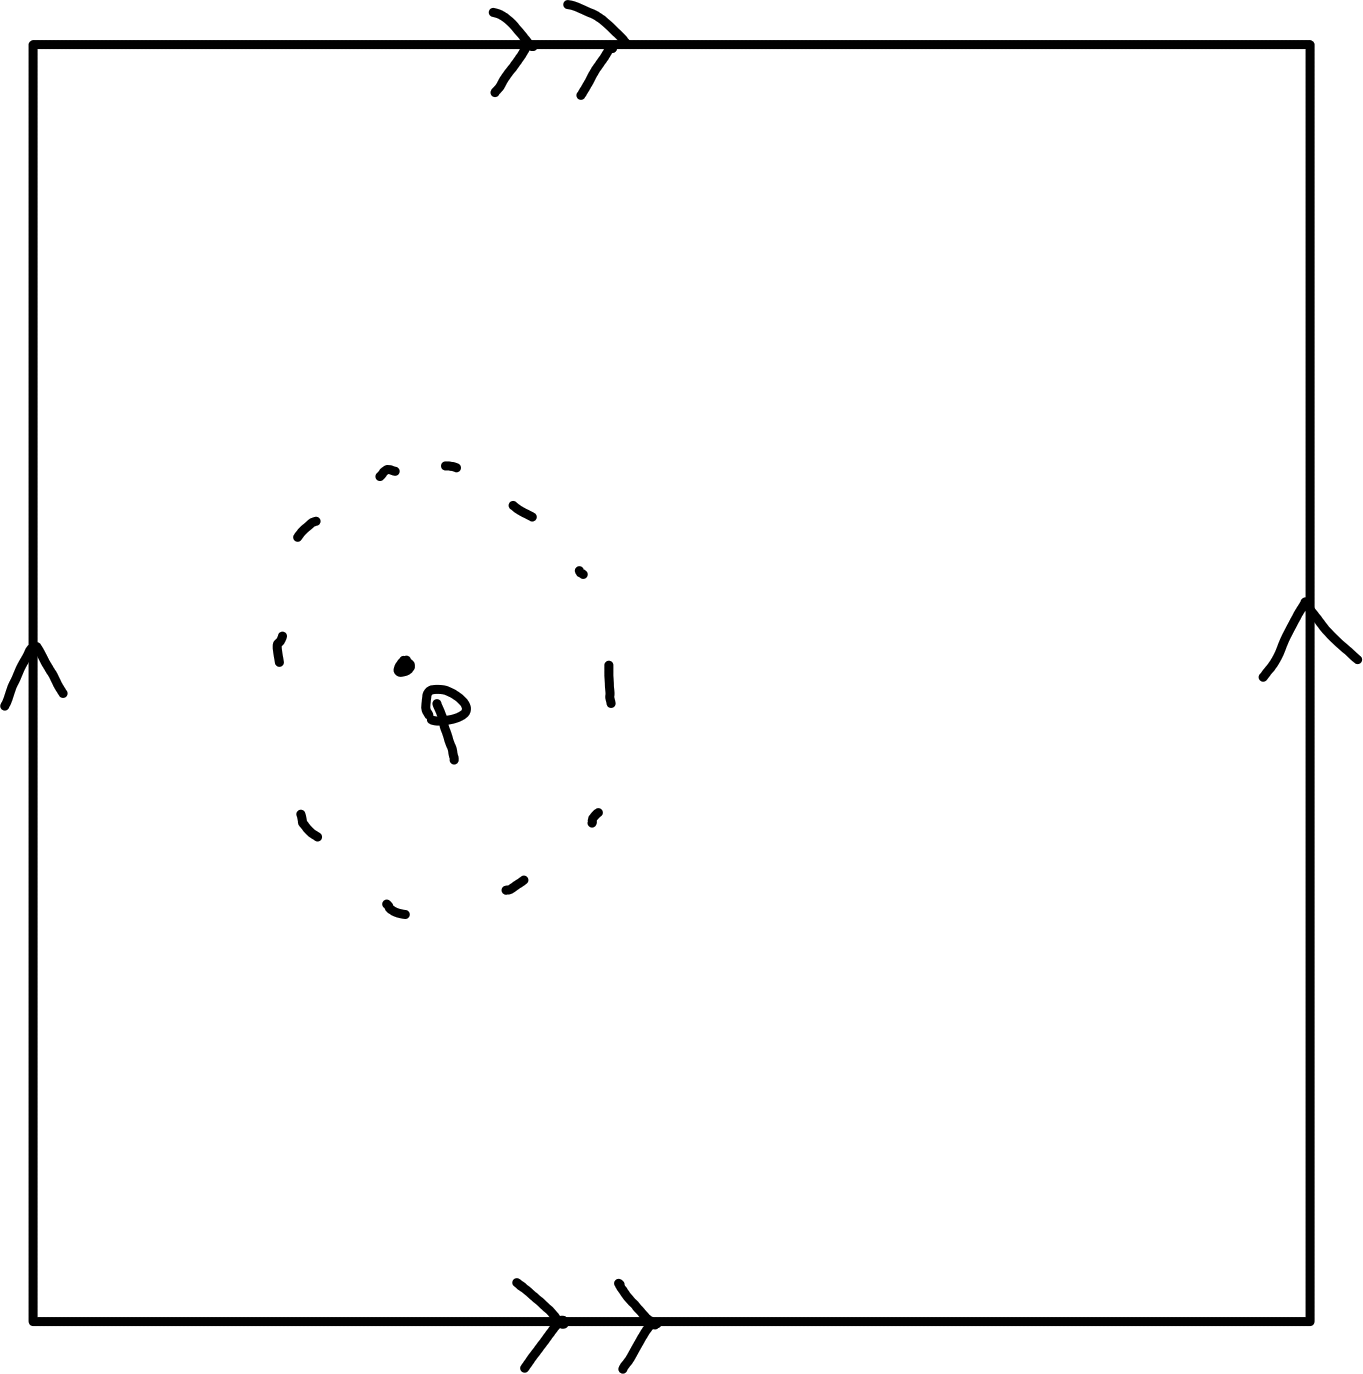
\includegraphics[height=3.5cm]{01-torussquare} 
		\par
	}

	Let $p$ be on an edge, but not a vertex.
	{ 	\par
		\centering 
		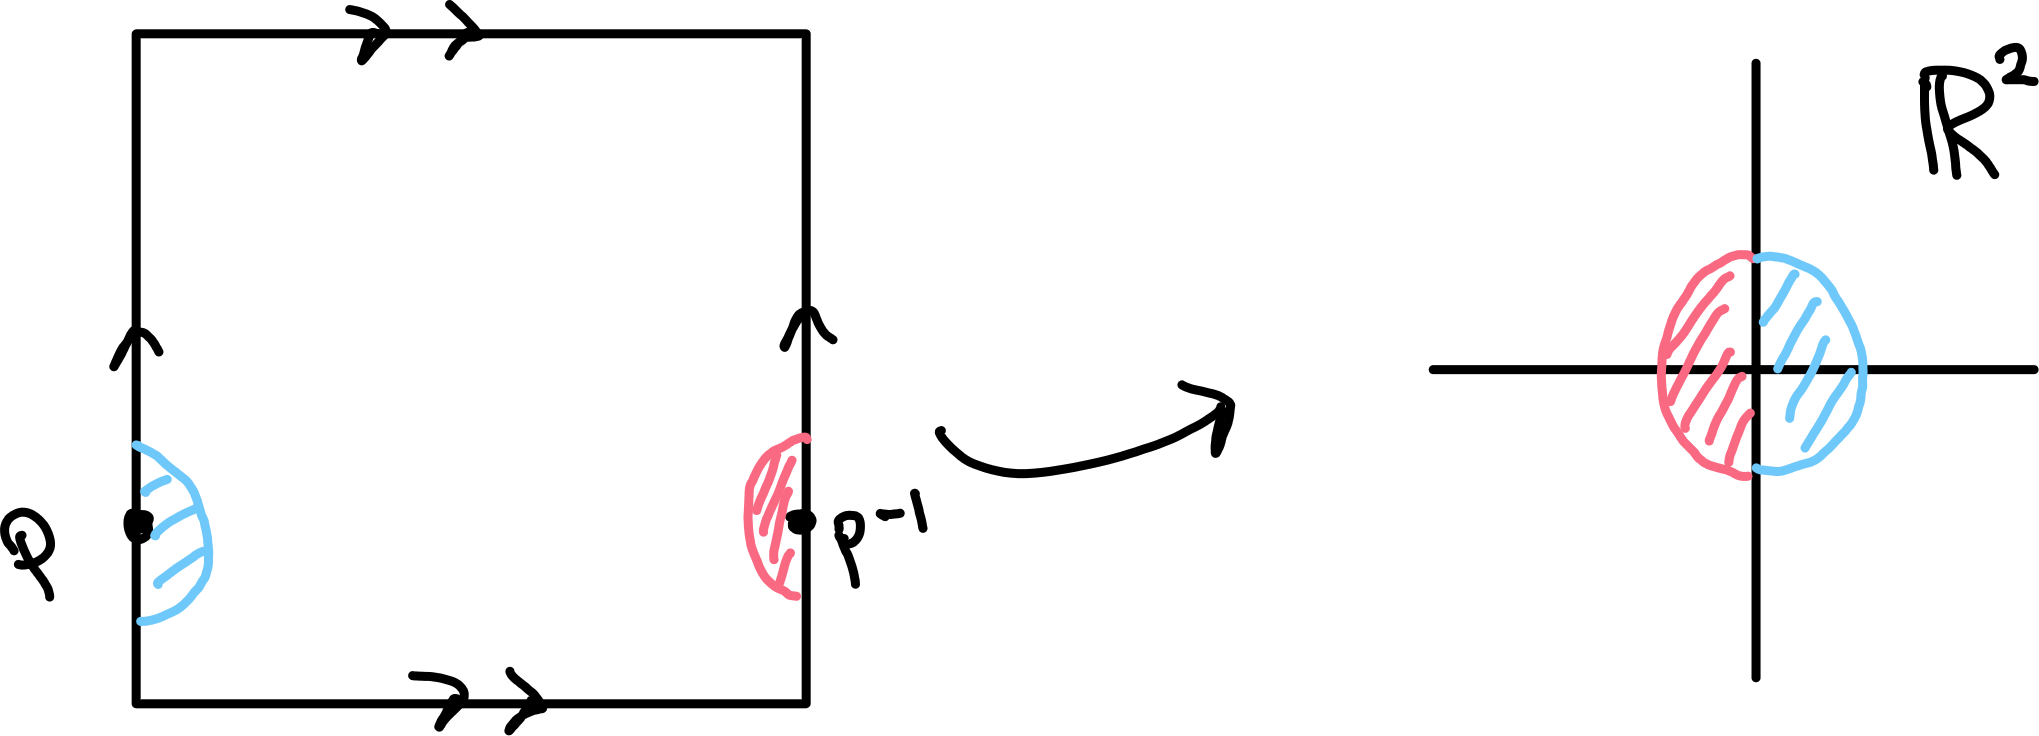
\includegraphics[height=5cm]{01-torussquare2} 
		\par
	}
	Let us say without loss of generality that $p = (0,y_0) \sim (1,y_0) = p'$.
	Let $\delta$ be sufficiently small that the closed half-discs $U, V$ centred on $p, p\inv$ with radius $\delta$ do not intersect any vertices. \\
	Then we define a map from the union of the two half-discs to the disc $B(0,\delta) \subset \mathbb R^2$ via 
	\begin{align*}
		U : (x,y) &\underset{f_u}{\mapsto} (x,y-y_0) \\
		V : (x,y) &\underset{f_v}{\mapsto} (x-1,y-y_0)
	\end{align*} which will be a bijective map.

	Recall the gluing lemma from Analysis and Topology: that if $X = A \cup B$ is a union of closed subspaces, and $f : A \to Y$, $g : B \to Y$ are continuous and $\eval{f}_{A \cap B} = \eval{g}_{A \cap B}$, they define a continuous map on $X$.

	$f_U, f_V$ are continuous on $U, V \subset [0, 1]^2$.
	By the definition of the quotient topology, $q \circ f_U$ and $q \circ f_V$ are also continuous ($q: [0, 1]^2 \to \faktor{[0, 1]^2}{\sim}$). \\
	In $T^2$, 1/2-discs, $q \circ U, q \circ V$ overlap but our maps agree as they are compatible with the equivalence relation. \\
	Hence, by the gluing lemma, $f_U, f_V$ ``glue'' together to give a continuous map to an open neighbourhood of $[p] \in T^2$ to $\mathbb{R}^2$.

	We can show that this is a homeomorphism using the usual process: pass to a closed disc, apply the topological inverse function theorem, then apply the result to the interior.
	If $[p] \in T^2$ lies in an edge on $P$, it has a neighbourhood homeomorphic to a disc.

	Now it suffices to consider points $p$ on a vertex.
	All four vertices of the square are identified to the same point in the torus as each vertex lies on two edges and so is identified to two other vertices.
	{ 	
		\par
		\centering 
		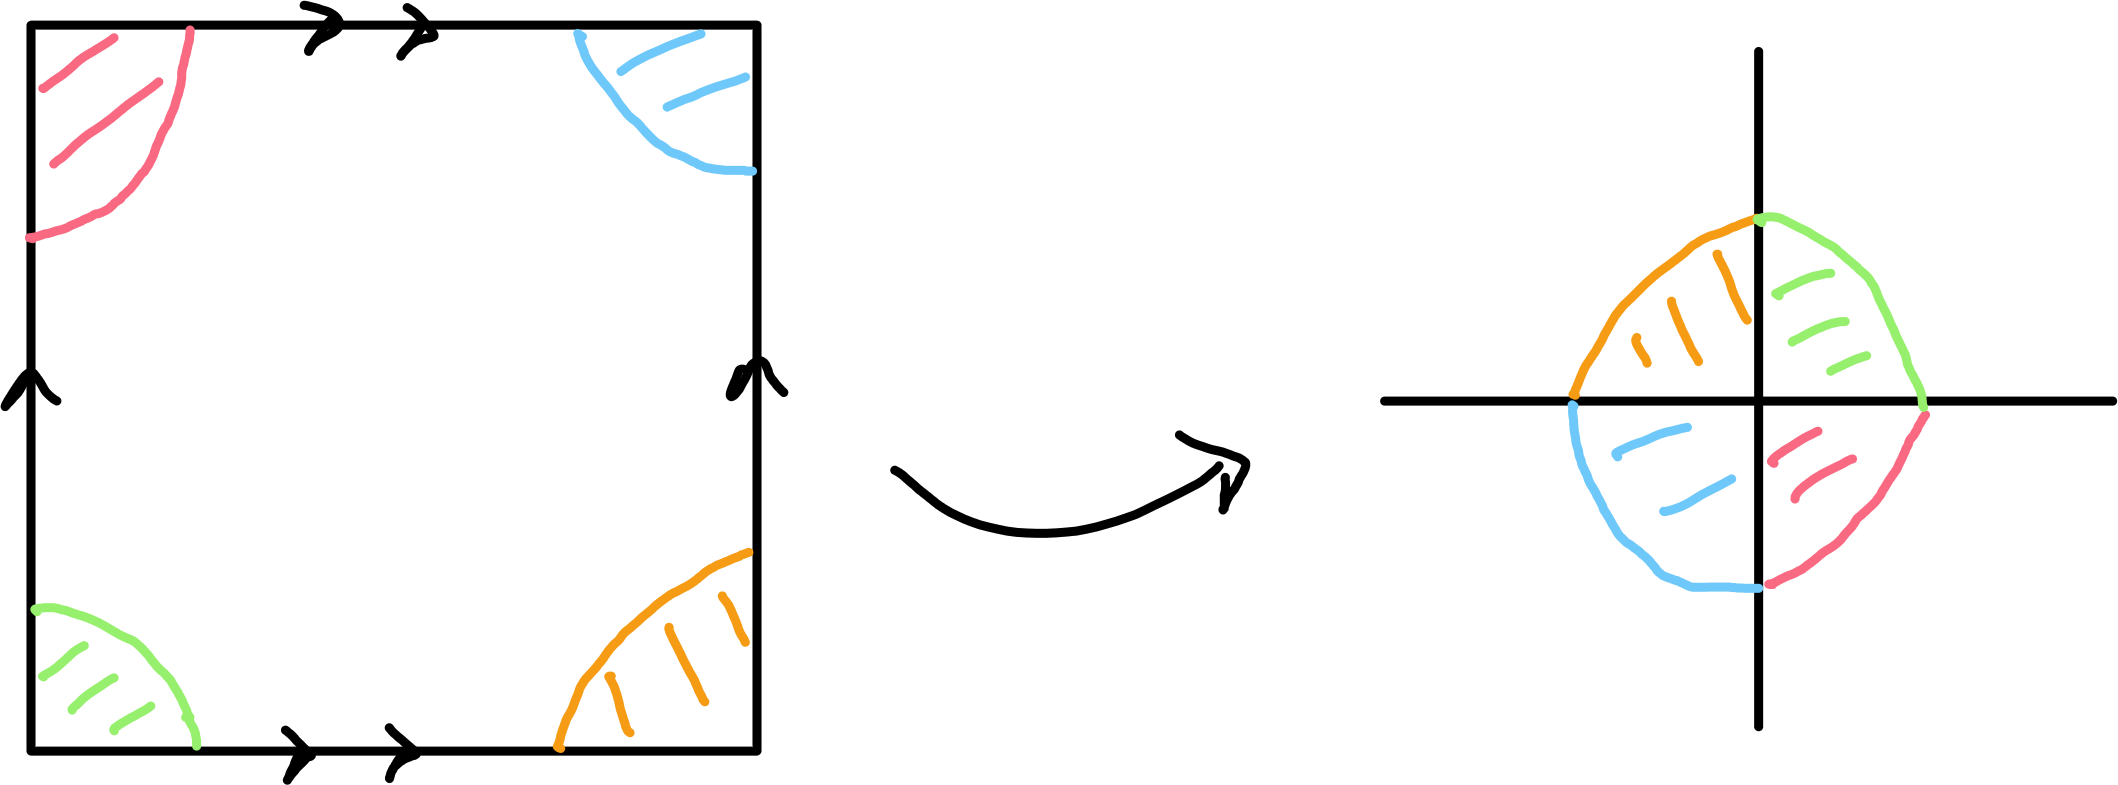
\includegraphics[height=5cm]{01-torussquare3} 
		\par
	}
	and analogously we get that a vertex has a neighbourhood homeomorphic to a disc.
	% A neighbourhood of each vertex can be identified with a quarter-disc in $\mathbb R^2$.
	% We can repeatedly apply the gluing lemma to construct the whole disc $B(0,\delta) \subset \mathbb R^2$ and complete the argument as before.

	Thus, $\faktor{[0,1]^2}{\sim}$ is a topological surface.
\end{example}

\begin{example}[General Polygon]
	We can generalise this proof to an arbitrary planar Euclidean polygon $P$, such as the hexagon above.
	The equivalence relation $x \sim f_{e \hat e}(x)$ induces an equivalence relation on the vertices of $P$, by considering the images of the vertices under all $f_{e\hat e}$.
	However, it is not necessarily the case that an equivalence class of vertices contains exactly four vertices, so quarter-discs are not necessarily applicable.
	Again, there are three types of point:
	\begin{itemize}
		\item interior points, for which a neighbourhood not intersecting the boundary is chosen;
		\item points on edges, for which a corresponding point exists and two half-discs can be glued to form the neighbourhood; and
		\item points on vertices.
		      For this case, all vertices of the polygon have a neighbourhood which is a sector of a circle.
		      Let there be $r$ vertices in a given equivalence class.
		      Let $\alpha$ be the sum of the angles of the sectors in a given class. \\
		      Any sector can be identified with a given sector in the disc $B(0,\delta) \subset \mathbb R^2$, which we will choose to have angle $\alpha / r$.
		      Then, we can glue each sector together in $\mathbb R^2$, compatibly with the orientations of the edges and arrows, inducing a neighbourhood which is locally homeomorphic to a disc.

		      If $r = 1$, we have an equivalence class comprising a single vertex, which gives a single sector.
		      For $r$ to be one, the two edges attached to this vertex must be paired and have the same direction (either both inwards or outwards from the vertex).
		      This quotient space is simply a cone, which is homeomorphic to a disc as required.
	\end{itemize}
	We can also show that the quotient space is Hausdorff and second countable.
	By construction, two distinct points in the quotient space can be separated by open neighbourhoods by selecting a sufficiently small radius such that the discs considered in the derivation above are disjoint.
	For second countability, consider
	\begin{itemize}
		\item discs in the interior of $P$ with rational centres and radii;
		\item for each edge of $P$, consider an isometry $e \to [0, \ell]$ where $\ell$ is the length of $e$, taking discs on $e$ which are centred at rational values in $[0,\ell]$; and
		\item for each vertex, consider discs centred at these vertices with rational radii.
	\end{itemize}
\end{example}

\begin{example}[Connected Sums]
	Given topological surfaces $\Sigma_1, \Sigma_2$ we can remove an open disc from each and glue the resulting boundary circles.
	{ 	
		\par
		\centering 
		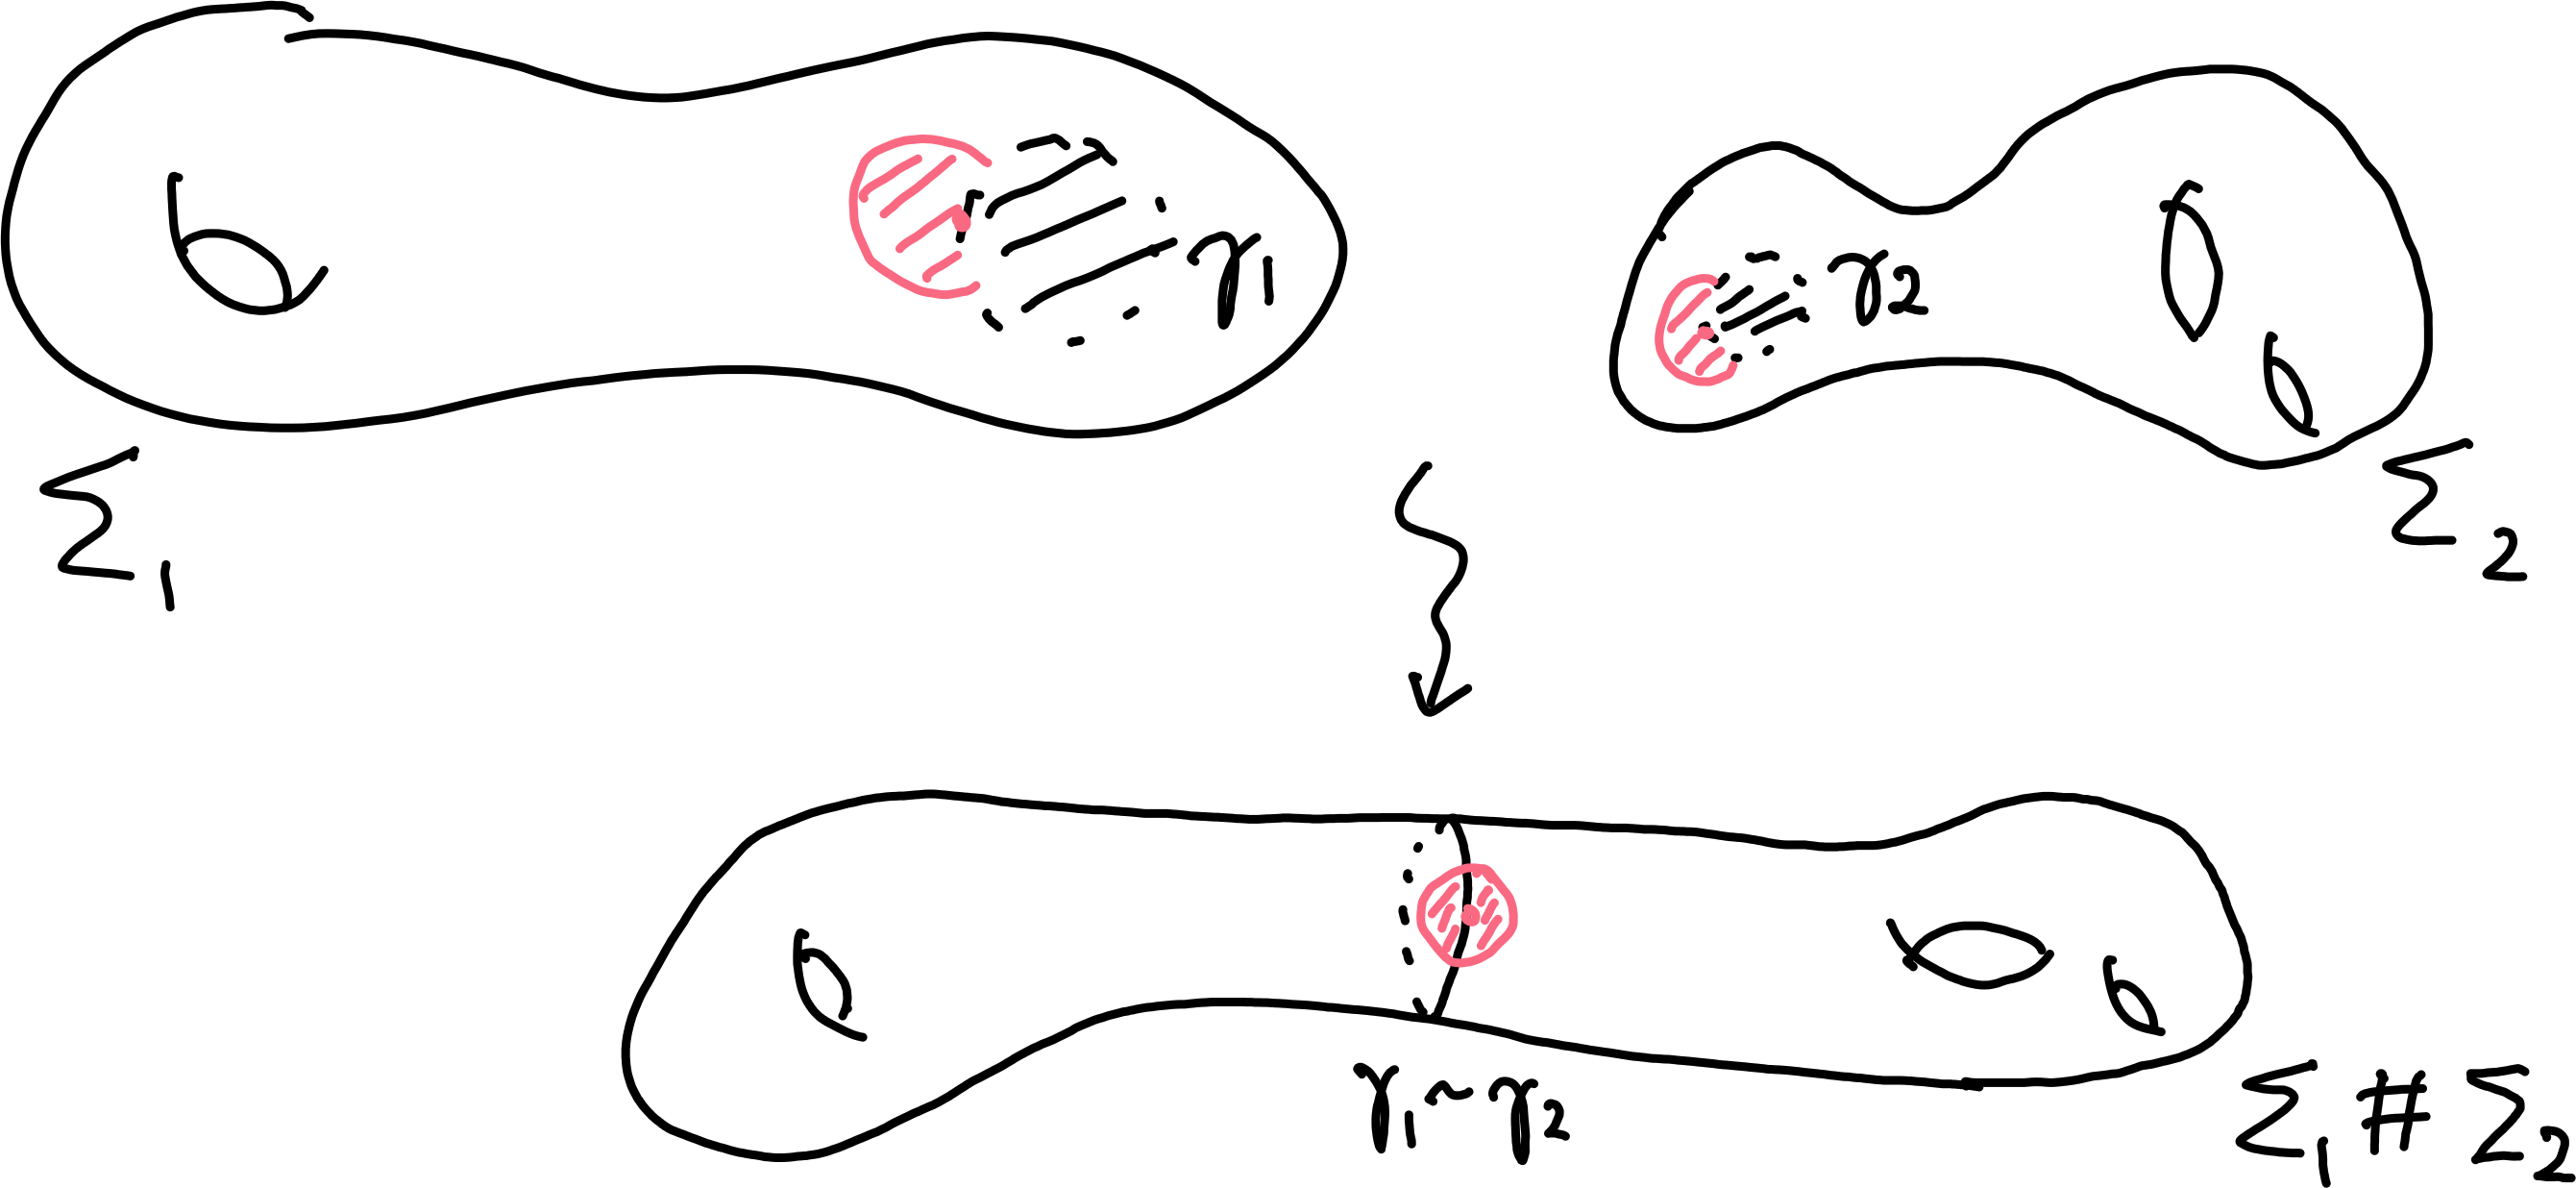
\includegraphics[height=5cm]{01-connectedsum} 
		\par
	}
	Explicitly, take $\Sigma_1 \setminus D_1 \indep\footnote{Disjoint Union} \Sigma_2 \setminus D_2$ and impose a quotient relation by identifying $\theta \in \partial D_1 \sim \theta \in \partial D_2$ where $\theta$ is an angle parametrising $S^1 = \partial D_i$, $\partial D_i$ is the boundary of $D_i$.
	The result $\Sigma_1 \connect \Sigma_2$ is called the \vocab{connected sum} of $\Sigma_1, \Sigma_2$.

	In principle this depends on many choices and takes some effort to prove that it is well-defined.

	% Typically, the information about where the discs were removed from is discarded when considering the connect sum.
	% The connect sum of two topological surfaces is a topological surface.
\end{example}

\begin{lemma}
	The connected sum $\Sigma_1 \connect \Sigma_2$ is a topological surface.
\end{lemma} 

\begin{proof}
	Not proved in this course, if you want to learn more try `Introduction to topological manifolds' by Jack Lee.
\end{proof} 

\begin{example}
	Consider the following octagon.
	\tikzfig{double_torus_polygon}
	The associated quotient space $\faktor{P}{\sim}$ can be seen to be homeomorphic to a surface with two holes, known as a double torus.
	All vertices are identified as the same vertex in the quotient space.
	We can cut the octagon along a diagonal, leaving two topological surfaces which are homeomorphic to a torus.
	\begin{center}
		\tikzfig{double_torus_polygon_expanded} $\mapsto$ \tikzfig{torus_polygon_with_loop}
	\end{center}
	Thus, the connected sum of the two half-octagons are the connected sum of two toruses.
\end{example}

\begin{example}
	Consider the following square.
	\tikzfig{rp2_polygon}
	This is homeomorphic to the real projective plane $\mathbb R \mathbb P^2$.
	This is because we identify points on the boundary with their antipodes, when interpreting the square as the closed disc $B(0,1)$.
	The real projective plane was constructed by identifying points on the unit sphere with their antipodes.
	Thus, we can construct a homeomorphism by considering only points in the upper hemisphere (taking antipodes as required), and then orthographically projecting onto the $xy$ plane.
	Under this transformation, points on the boundary are identified with their antipodes as required.
\end{example}

\subsection{Subdivisions}

\begin{definition}[Subdivision]
	A \vocab{subdivision} of a compact topological surface $\Sigma$ comprises
	\begin{enumerate}
		\item a finite subset $V \subset \Sigma$ of vertices;
		\item a finite subset of edges $E = \qty{e_i : [0,1] \to \Sigma}$ s.t. 1) each $e_i$ is a continuous injection on its interior and $e_i\inv V = \{0, 1\}$, the endpoints.
		2) $e_i, e_j$ have disjoint images except perhaps at their endpoints.
		\item we require that each connected component of $\Sigma \setminus \qty(\cup_i e_i [0, 1] \cup V)$ is homeomorphic to an open disc called a \vocab{face}.
		      In particular, the closure of a face has boundary $\overline F \setminus F$ lying in $\qty(\cup_i e_i [0, 1] \cup V)$.
	\end{enumerate}
\end{definition}

\begin{definition}[Triangulation]
	We say that a subdivision is a \vocab{triangulation} if each closed face (closure of a face) contains exactly three edges, and two closed faces are disjoint, meet at exactly one edge or just one vertex.
\end{definition} 

\begin{example}
	A cube displays a subdivision of $S^2$.
	A tetrahedron displays a triangulation of $S^2$.
\end{example}

\begin{example}
	We can display subdivisions of surfaces constructed from polygons.
	\tikzfig{torus_polygon}
	This is a subdivision of a torus with one vertex, two edges, and one face.
	We can construct additional subdivisions of a torus, for example:
	\begin{center}
		\tikzfig{torus_polygon_subdivided} \quad \tikzfig{torus_polygon_triangulated}
	\end{center}
	The first of these examples is not a triangulation, since the two faces meet in more than one edge.
	The second is a triangulation.
\end{example}

\begin{remark}
	The following is a very degenerate subdivision of $S_2$.
	\tikzfig{s2_degenerate}\footnote{This is not a circle, its a 2-sphere.}
	This has one vertex, no edges, and one face.
\end{remark}

\subsection{Euler classification}
\begin{definition}[Euler Characteristic]
	The \vocab{Euler characteristic} of a subdivision is
	\begin{align*}
		\#\footnote{The number/size of the set} V - \# E + \# F
	\end{align*}
\end{definition}

\begin{theorem}
	\begin{enumerate}
		\item Every compact topological surface has a subdivision (and indeed triangulations).
		\item The Euler characteristic is invariant under choice of subdivision, and is topologically invariant of the surface (depends only on the homeomorphism type of $\Sigma$).
	\end{enumerate}
	Hence, we might say that a surface has a particular Euler characteristic, without referring to subdivisions.
	We write this $\chi(\Sigma)$.
\end{theorem}

\begin{remark}
	It is not trivial to prove part (i).
	For part (ii), note that subdivisions can be converted into triangulations by constructing triangle fans.
	\tikzfig{triangle_fan}
	Triangulations can be related by local moves, such as
	\tikzfig{triangulation_local_move}
	It is easy to check that both of these moves do not change the Euler characteristic.
	However, it is hard to make this argument rigorous, and it does not give much explanation for why the result is true.
	In Part II Algebraic Topology, a more advanced definition of the Euler characteristic is given, which admits a more elegant proof.
\end{remark}

\begin{proof}
	No proof will be given.
\end{proof} 

\begin{example}
	The Euler characteristic of $S^2$ is $\chi(S^2) = 2$.
\end{example}

\begin{example}
	For the torus, $\chi(T^2) = 0$.
\end{example} 

\begin{example}
	If $\Sigma_1, \Sigma_2$ are compact surfaces, then the connected sum $\Sigma_1 \connect \Sigma_2$ can be constructed by removing a face of a triangulation, then gluing together the boundary circles (three edges) in a way that matches the edges.

	Then the connected sum inherits a subdivision, and we can find that it has Euler characteristic $\chi(\Sigma_1 \connect \Sigma_2) = \chi(\Sigma_1) + \chi(\Sigma_2) - 2$, where the remaining term corresponds to the two faces that were removed; the changes of three vertices and three edges cancel each other.

	In particular, a surface $\Sigma_g$ with $g$ holes can be written $\bigconnect_{i=1}^g T^2$, so $\chi(\Sigma_g) = 2 - 2g$.
	We call $g$ the \vocab{genus} of $\Sigma$.
\end{example} 
    \section{Abstract smooth surfaces}

\subsection{Charts and atlases}
Recall that if $\Sigma$ is a topological surface, any point lies in an open neighbourhood homeomorphic to a disc.

\begin{definition}[Chart]
	A pair $(U, \varphi)$, where $U$ is an open set in $\Sigma$ and $\varphi \colon U \to V$ is a homeomorphism to an open set $V \subseteq \mathbb R^2$, is called a \vocab{chart} for $\Sigma$.
	If $p \in U$, we might say that $(U, \varphi)$ is a chart for $\Sigma$ \textit{at $p$}.
\end{definition}

\begin{definition}[Local parameterisation]
	The inverse $\sigma = \varphi^{-1} \colon V \to U$ is known as a \vocab{local parametrisation} for the surface.
\end{definition} 

\begin{definition}[Atlas]
	A collection of charts $\{ (U_i, \phi_i)_{i \in I}\}$ whose domains cover $\Sigma$ ($\cup_{i \in I} U_i = \Sigma$) is known as an \vocab{atlas} for $\Sigma$.
\end{definition} 

\begin{example}
	If $Z \subseteq \mathbb R^2$ is closed, $\mathbb R^2 \setminus Z$ is a topological surface with an atlas containing one chart, $(\mathbb R^2 \setminus Z, \phi = \id)$.
\end{example}

\begin{example}
	For $S^2$, there is an atlas with two charts, which are the two stereographic projections from the poles.
	% We could consider alternative charts, for instance the projection to the $yz$ plane, but this would be insufficient for describing the poles.
\end{example} 

\begin{definition}[Transition Map]
	Let $(U_i, \varphi_i)$ be charts containing the point $p \in \Sigma$, for $i = 1, 2$.
	Then the map
	\begin{align*}
		\varphi_2 \circ \eval{\varphi_1^{-1}}_{\varphi_1(U_1 \cap U_2)} : \varphi_1(U_1 \cap U_2) \to \varphi_2(U_1 \cap U_2)
	\end{align*}
	converts between the corresponding charts, and is called a \textit{transition map} between charts.
	This is a homeomorphism of open sets in $\mathbb R^2$.
\end{definition}

\begin{figure}[h] 
    \centering 
    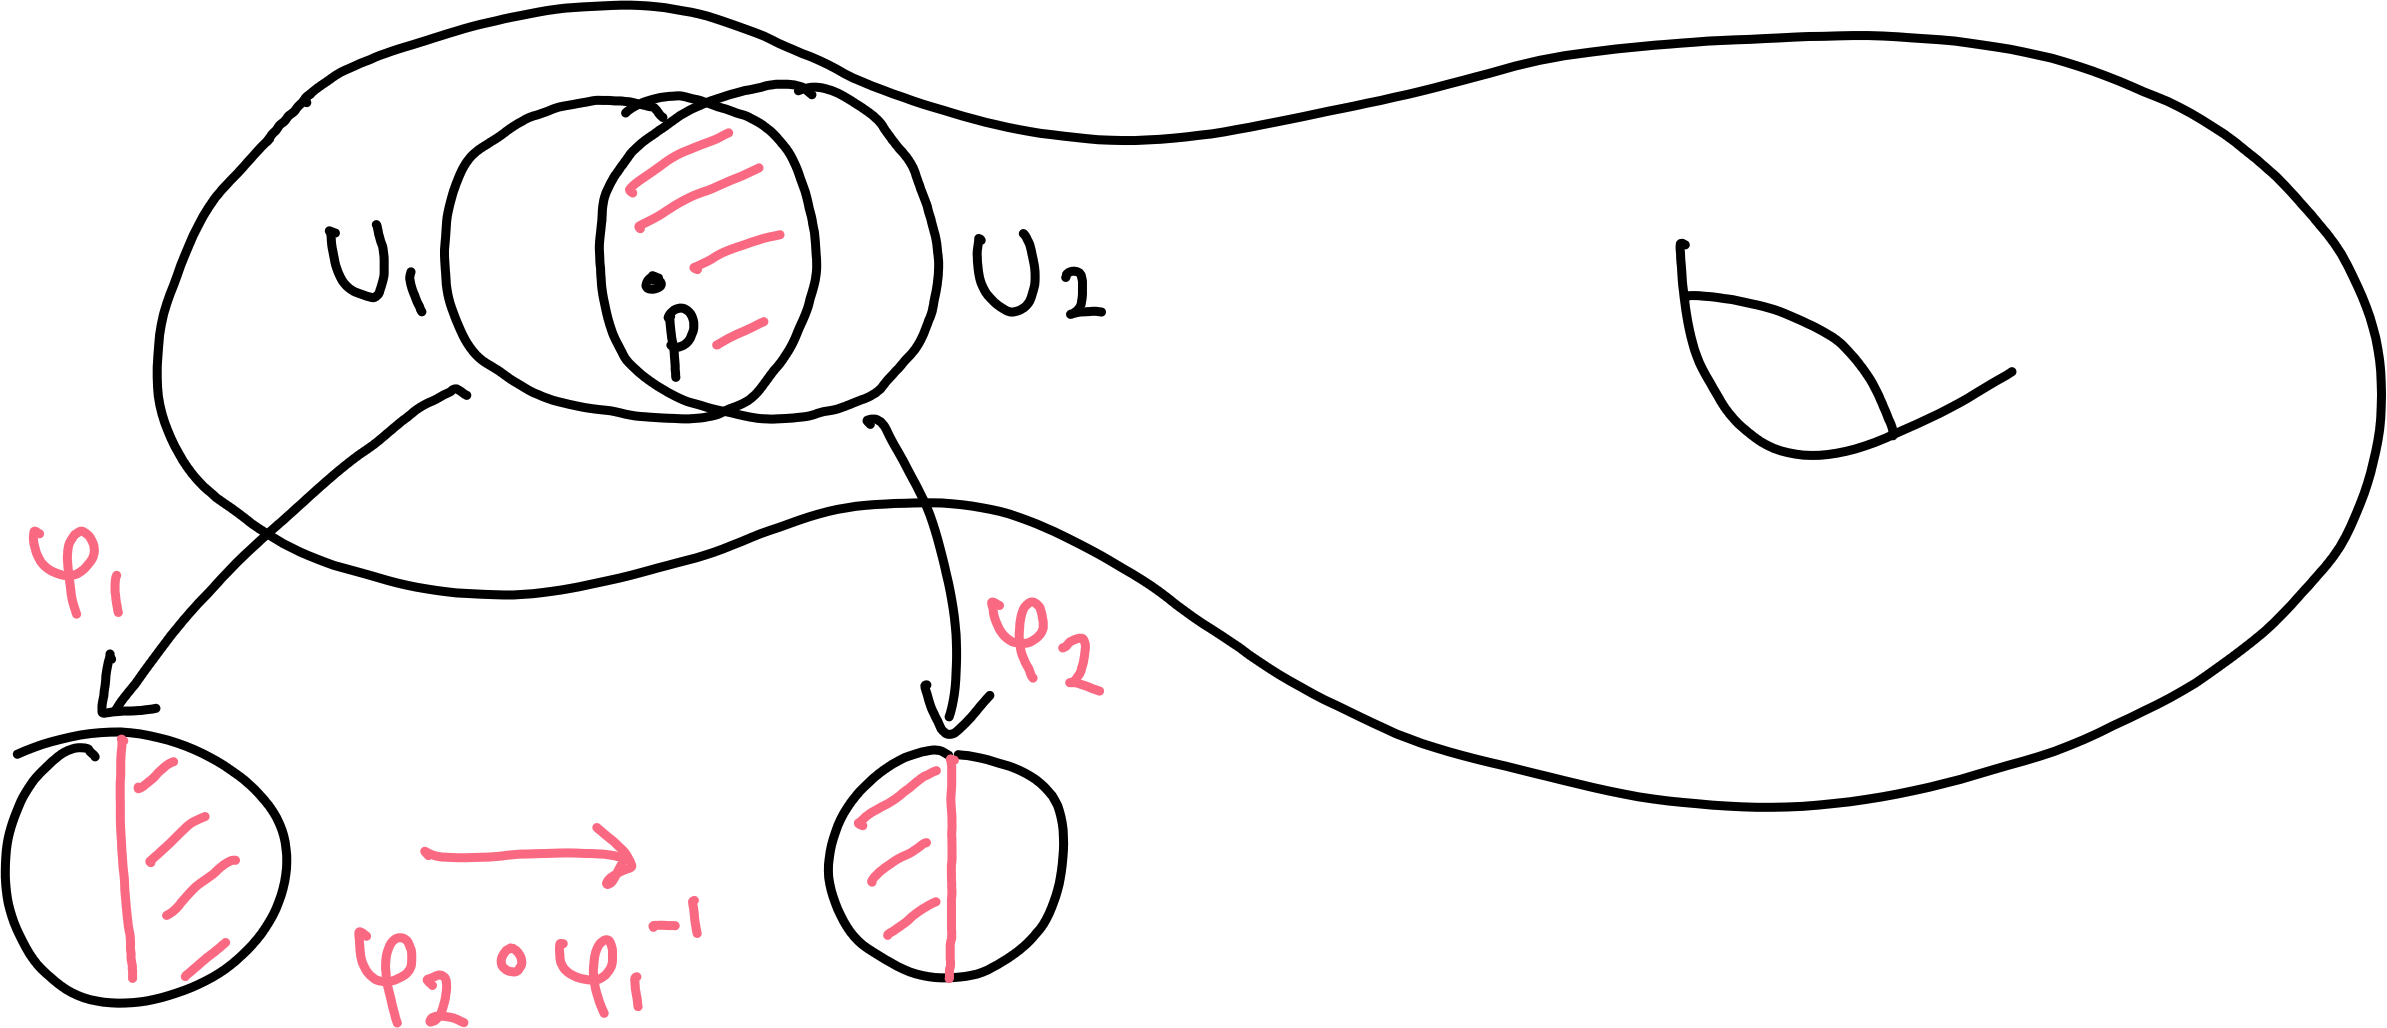
\includegraphics[height=5cm]{02-transition} 
\end{figure}

Recall from Analysis and Topology that if $V \subseteq \mathbb R^n$ and $V' \subseteq \mathbb R^m$ are open, then a continuous map $f \colon V \to V'$ is called \textit{smooth} if it is infinitely differentiable.
Equivalently, it is smooth if continuous partial derivatives of all orders in all variables exist at all points.

\begin{definition}[Diffeomorphism]
	A homeomorphism $f : V \to V'$ is called a \vocab{diffeomorphism} if it is smooth and it has a smooth inverse.
\end{definition} 

\begin{definition}[Abstract Smooth Surface]
	An \vocab{abstract smooth surface} $\Sigma$ is a topological space with an atlas of charts $\{(U_i, \varphi_i)_{i \in I}\}$ s.t. all transition maps are diffeomorphisms.
\end{definition}

\begin{remark}
	We could not simply consider a smoothness condition for $\Sigma$ itself without appealing to atlases, since $\Sigma$ is an arbitrary topological space and could have almost any topology.
\end{remark}

\begin{example}
	The atlas of two charts with stereographic projections gives $S^2$ the structure of an abstract smooth surface.
\end{example}

\begin{example}
	For the torus $T^2 = \faktor{\mathbb R^2}{\mathbb Z^2}$, we can find charts of all points by choosing sufficiently small discs in $\mathbb R^2$ such that they do not intersect any of their non-trivial integer translates.
	The transition maps for this atlas are all translations of $\mathbb R^2$.
	Hence $T^2$ inherits the structure of an abstract smooth surface.
	Explicitly, let us define $e \colon \mathbb R^2 \to T^2$ by $(t,s) \mapsto \qty(e^{2\pi i t}, e^{2 \pi i s})$, then consider the atlas
	\begin{align*}
		\qty{(e\qty(D_\varepsilon(x,y)), e^{-1} \text{ on this image})}
	\end{align*}
	for $\varepsilon < \frac{1}{3}$.
	These are charts on $T^2$, and the transition maps are (restricted to appropriate domains) translations in $\mathbb R^2$.
	Hence $T^2$, via this atlas, has the structure of an abstract smooth surface.
\end{example}
\begin{remark}
	The definition of a topological surface is a notion of structure.
	One can observe a topological space and determine whether it is a topological surface.
	Conversely, to be an abstract smooth surface is to have a specific set of data; that is, we must provide charts for the surface in order to see that it is indeed an abstract smooth surface.
\end{remark}
\begin{definition}
	Let $\Sigma$ be an abstract smooth surface, and $f \colon \Sigma \to \mathbb R^n$ be a continuous map.
	We say that $f$ is \textit{smooth} at $p \in \Sigma$ if, for all charts $(U, \varphi)$ of $p$ belonging to the smooth atlas for $\Sigma$, the map
	\begin{align*}
		f \circ \varphi^{-1} \colon \varphi(U) \to \mathbb R^n
	\end{align*}
	is smooth at $\varphi(p) \in \mathbb R^2$.
\end{definition}
\begin{remark}
	Note that the choice of chart and atlas was arbitrary, but smoothness of $f$ at $p$ is independent of the choice of chart, since the transition maps between two such charts are diffeomorphisms.
\end{remark}
\begin{definition}
	Let $\Sigma_1, \Sigma_2$ be abstract smooth surfaces.
	Then a map $f \colon \Sigma_1 \to \Sigma_2$ is \textit{smooth} if it is `smooth in the local charts'.
	Given a chart $(U, \varphi)$ at $p$ and a chart $(U', \psi)$ at $f(p)$, both mapping to open subsets of $\mathbb R^2$, the map $\psi \circ f \circ \varphi^{-1}$ is smooth at $\varphi(p)$.
	Smoothness of $f$ does not depend on the choice of chart, provided that the charts all belong to the same atlas.
\end{definition}
\begin{definition}
	Two surfaces $\Sigma_1, \Sigma_2$ are \textit{diffeomorphic} if there exists a homeomorphism $f \colon \Sigma_1 \to \Sigma_2$ which is smooth and has smooth inverse.
\end{definition}
\begin{remark}
	Often, we convert from a given smooth atlas for an abstract smooth surface $\Sigma$ to the \textit{maximal compatible} smooth atlas.
	That is, we consider the atlas with the maximal possible set of charts, all of which have transition maps that are diffeomorphisms.
	This can be accomplished formally by use of Zorn's lemma.
\end{remark}

    \section{Smooth surfaces in $\mathbb R^3$}

\subsection{Definitions and equivalent characterisations}
Recall that if $V \subset \mathbb R^n$ and $V' \subset \mathbb R^m$, then $f \colon V \to V'$ is smooth if it is infinitely differentiable.

\begin{definition}[Smooth Function on $\mathbb{R}^n$]
	If $Z$ is an arbitrary subset of $\mathbb R^n$, we say that $f \colon Z \to \mathbb R^m$ is \vocab{smooth} at $p \in Z$ if $\exists$ an open ball $p \in B \subset \mathbb R^n$ and a smooth map $F \colon B \to \mathbb R^m$ which extends $f$ such that they agree on $B \cap Z$\footnote{$F\mid_{B \cap Z} = f\mid_{B \cap Z}$}.
	In other words, $f$ is locally the restriction of a smooth map defined on an open set.
\end{definition}

\begin{remark}
	This is useful as it may be difficult to take partial derivatives on $Z$, as when you consider a small deviation from a point $p$ that deviation might not lie in $Z$.
\end{remark} 

\begin{figure}[h] 
    \centering 
    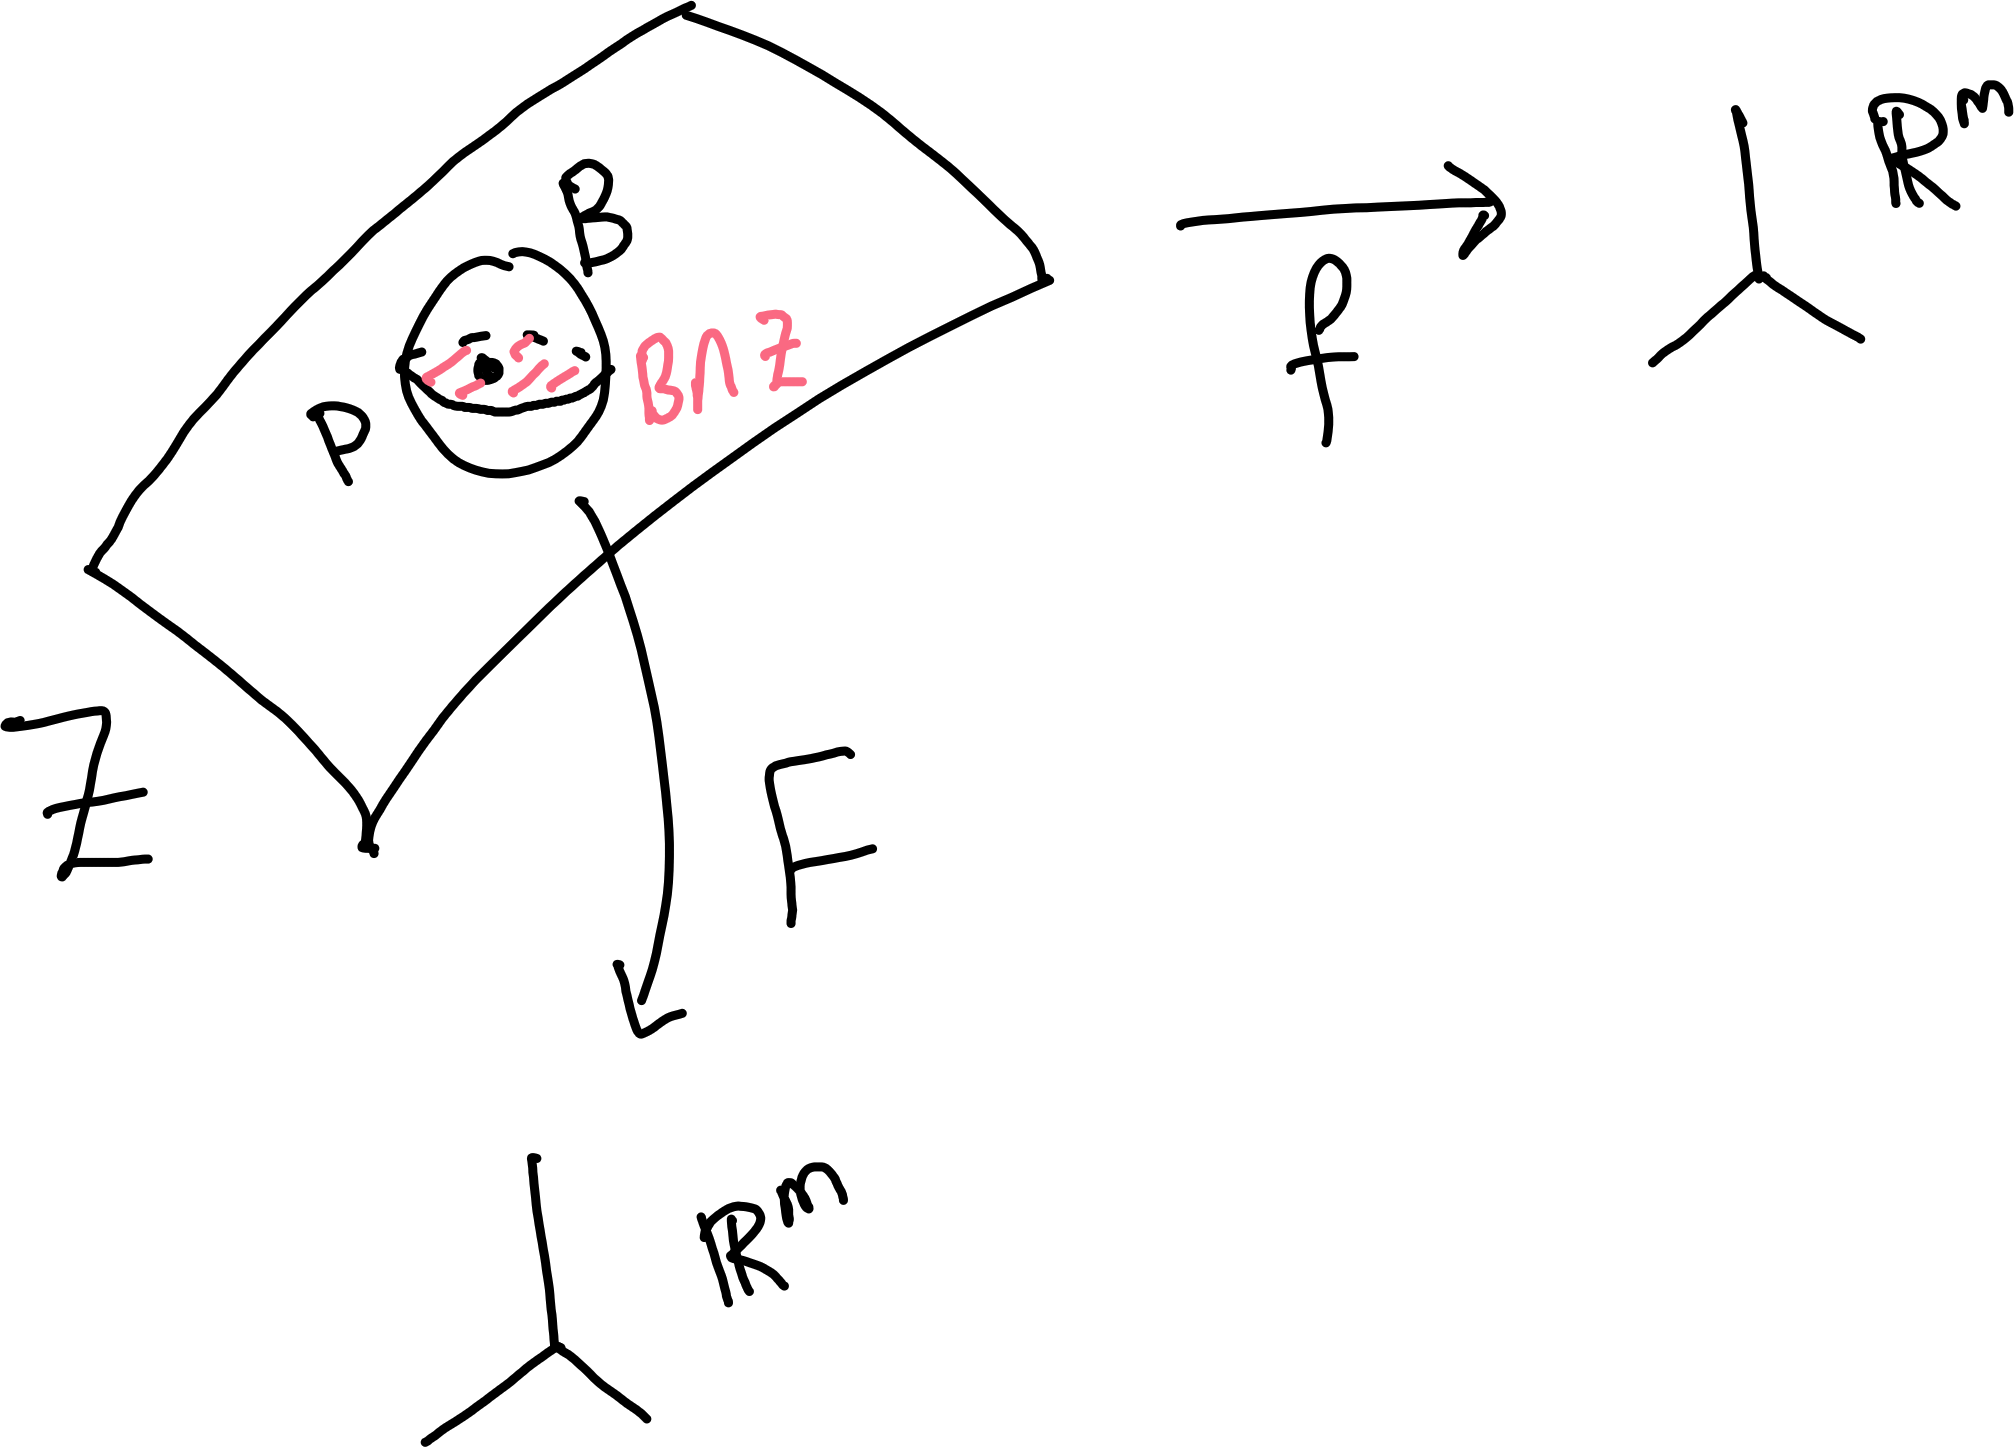
\includegraphics[height=5cm]{03-smooth} 
\end{figure}

\begin{definition}[Diffeormorpishms in $\mathbb{R}^n, \mathbb{R}^m$]
	Let $X \subset \mathbb R^n$ and $Y \subset \mathbb R^m$.
	We say that $X$ and $Y$ are \vocab{diffeomorphic} if $\exists \; f \colon X \to Y$ smooth with smooth inverse.
\end{definition}

\begin{definition}[Smooth Surface in $\mathbb{R}^3$]
	A \vocab{smooth surface in $\mathbb R^3$} is a subset of $\Sigma \subset \mathbb R^3$ s.t. $\forall \; p \in \Sigma$, $\exists$ an open subset $p \in U \subset \Sigma$ that is diffeomorphic to an open set in $\mathbb R^2$.
\end{definition}

In other words, for all $p \in \Sigma$, there exists an open ball $p \in B \subset \mathbb R^3$ such that if $U = B \cap \Sigma$ and there exists a map $F \colon B \to V \subset \mathbb R^2$ smooth s.t. $\eval{F}_U \colon U \to V$ is a homeomorphism, and the inverse map $V \to U \subset \Sigma \subset \mathbb R^3$ is smooth.

So we have two notions of smoothness, one abstract and one based on the ambient space and we need to reconcile them.

\begin{definition}[Allowable Parameterisation]
	Let $\sigma \colon V \to U$ where $V \subset \mathbb R^2$ is open and $U \subset \Sigma \subset \mathbb R^3$ is open in $\Sigma$, such that $\sigma$ is a smooth homeomorphism and $\eval{D\sigma}_x$ has rank 2 for all $x \in V$.
	Then $\sigma$ is called an \vocab{allowable parametrisation}.
	If $\sigma(0) = p$, we say that $\sigma$ is an allowable parametrisation \textit{near} $p$.
\end{definition}

\begin{theorem} \label{thm:1.7}
	For a subset $\Sigma \subset \mathbb R^3$, the following are equivalent (TFAE).
	\begin{enumerate}
		\item $\Sigma$ is a smooth surface in $\mathbb R^3$;
		\item $\Sigma$ is locally the graph of a smooth function, over one of the three coordinate planes: for all $p \in \Sigma$ there exists an open ball $p \in B \subset \mathbb R^3$ and an open set $V \subset \mathbb R^2$ such that
		      \begin{align*}
			      \Sigma \cap B = \qty{(x, y, g(x,y)) \colon g \colon V \to \mathbb R \text{ smooth}}
		      \end{align*}
		      or one of the other coordinate planes;
		\item $\Sigma$ is locally cut out by a smooth function with non-zero derivative: for all $p \in \Sigma$ there exists an open ball $p \in B \subset \mathbb R^3$ and a smooth function $f \colon B \to \mathbb R$ such that
		      \begin{align*}
			      \Sigma \cap B = f^{-1}(0);\quad \eval{Df}_x \neq 0 \ \forall \; x \in B.
		      \end{align*}
		\item $\Sigma$ is locally the image of an allowable parametrisation near all points.
	\end{enumerate}
\end{theorem}

\begin{remark}
	Part (2) implies that if $\Sigma$ is a smooth surface in $\mathbb R^3$, each $p \in \Sigma$ belongs to a chart $(U, \varphi)$ where $\varphi$ is (the restriction of) one of the three coordinate plane projections $\pi_{xy}, \pi_{yz}, \pi_{xz}$ from $\mathbb R^3$ to $\mathbb R^2$.
	Consider the transition map between two such charts.
	{\par
	\centering 
    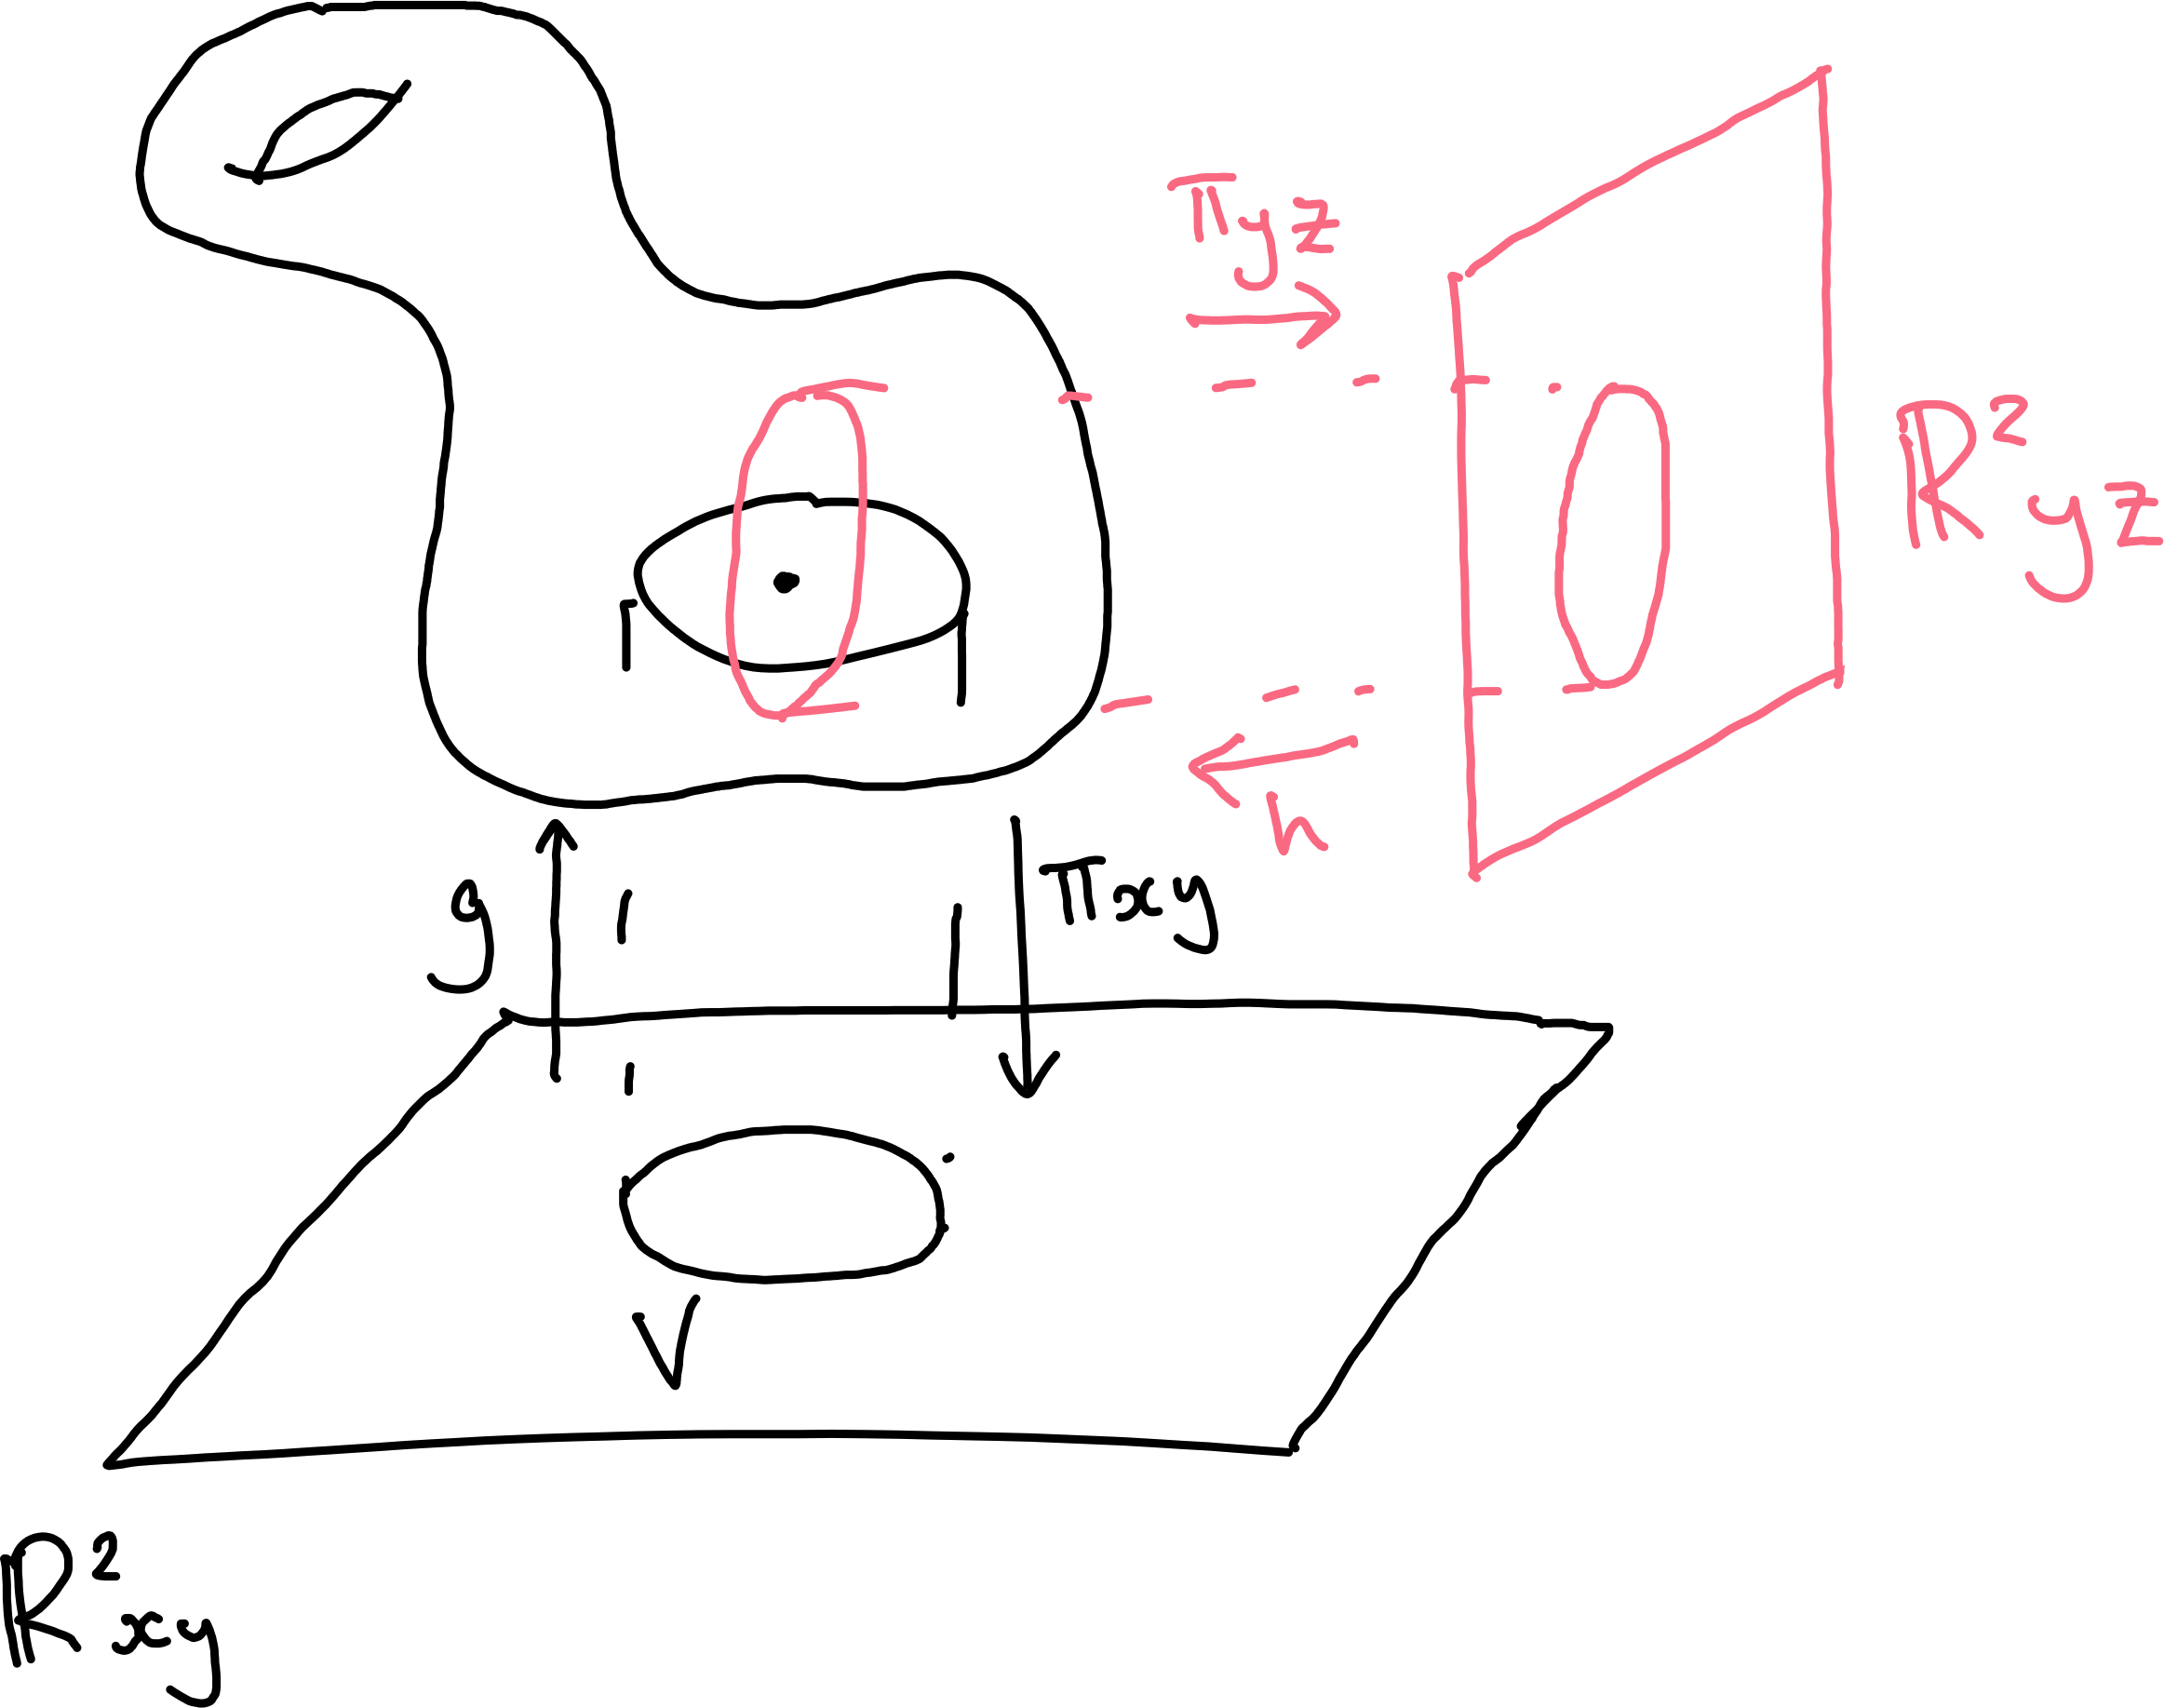
\includegraphics[height=5cm]{03-transitionmapremarks} 
	\par}
	If the two charts are based on the same projection such as $\pi_{xy}$, then the transition map is the identity.
	If they are based on different projections $\pi_{xy}$ and $\pi_{yz}$, then the transition map is
	\begin{align*}
		(x,y) \mapsto (x,y,g(x,y)) \mapsto (y,g(x,y))
	\end{align*}
	which has inverse
	\begin{align*}
		(y,z) \mapsto (h(y,z),y,z) \mapsto (h(y,z),y)
	\end{align*}
	Hence all of the transition maps between such charts are smooth.
	This gives $\Sigma$ the structure of an abstract smooth surface.
\end{remark}
Some of the relations given in the above theorem are easy to prove, but others come as a result of the inverse function theorem.

\subsection{Inverse and implicit function theorems}
\begin{theorem}[Inverse Function Theorem]
	Let $U \subset \mathbb R^n$ be open, and $f \colon U \to \mathbb R^n$ be continuously differentiable.
	Let $p \in U$ and $f(p) = q$.
	Suppose $\eval{Df}_p$ is invertible. \\
	Then there is an open neighbourhood $V$ of $q$ and a differentiable map $g \colon V \to \mathbb R^n$ and $g(q) = p$ with image an open neighbourhood $U' \subset U$ of $p$ such that $f \circ g = \id_V$ and $g \circ f = \id_{U'}$.
	If $f$ is smooth, then $g$ is also.
\end{theorem}

\begin{remark}
	The chain rule then implies that $\eval{Dg}_q = \qty(\eval{Df}_p)^{-1}$.

	The inverse function theorem concerns functions $\mathbb R^n \to \mathbb R^n$, where $\eval{Df}_p$ is an isomorphism.
	If we have a map $\mathbb R^n \to \mathbb R^m$ for $n > m$, then we can discuss the behaviour when $\eval{Df}_p$ is surjective.
	The derivative $\eval{Df}_p$ is an $m \times n$ matrix, so if it has full rank, up to the permutation of coordinates we have that the last $m$ columns are linearly independent.
\end{remark}

\begin{theorem}[Implicit Function Theorem]
	Let $p = (x_0, y_0)$ be a point in an open set $U \subset \mathbb R^k \times \mathbb R^\ell$.
	Let $f \colon U \to \mathbb R^\ell$ be a continuously differentiable map s.t. $p \mapsto 0$ and $\qty(\pdv{f_i}{y_j})_{\ell \times \ell}$ is an isomorphism at $p$. \\
	Then there is an open neighbourhood $V$ of $x_0$ in $\mathbb R^k$ and a continuously differentiable map $g \colon V \to \mathbb R^\ell$ with $x_0 \mapsto y_0$ such that if $(x,y) \in U \cap (V \times \mathbb R^\ell)$, then $f(x,y)=0 \iff y=g(x)$.
	If $f$ is smooth, so is $g$.
\end{theorem}

\begin{proof}
	Let $F \colon U \to \mathbb R^k \times \mathbb R^\ell$ be defined by $(x,y) \mapsto (x,f(x,y))$.
	Then note that
	\begin{align*}
		DF = \begin{pmatrix}
			I & \ast           \\
			0 & \pdv{f_i}{y_j}
		\end{pmatrix}
	\end{align*}
	hence $DF$ is an isomorphism at $(x_0, y_0)$.
	By the Inverse function theorem, $F$ is locally invertible near $F(x_0,y_0) = (x_0,f(x_0,y_0)) = (x_0, 0)$. \\
	Consider an open neighbourhood $(x_0, 0) \in V \times V' \subset \mathbb R^k \times \mathbb R^\ell$, where $V, V'$ open, on which this continuously differentiable inverse $G \colon V \times V' \to U' \subset U \subset \mathbb R^k \times \mathbb R^\ell$ exists, such that $F \circ G = \id_{V \times V'}$. \\
	Then,
	\begin{align*}
		G(x,y) = (\varphi(x,y), \psi(x,y)) \implies F \circ G(x,y) = (\varphi(x,y), f(\varphi(x,y), \psi(x,y))) = (x,y)
	\end{align*}
	Hence $\varphi(x,y) = x$.
	We have $f(x,\psi(x,y)) = y$ when $(x,y) \in V \times V'$.
	This gives $f(x,y) = 0 \iff y = \psi(x,0)$\footnote{Here $y$ is in $V'$ so it is in the image of $f$, i.e. it is $f(a, b)$ for some $a, b$. So $y = 0$ gives us $f(a, b) = 0$. We see that $f(a, \psi(a, 0)) = 0$ so $b = \psi(a, 0)$ defines our surface in $U$}. \\
	We then define $g \colon V \to \mathbb R^\ell$ by $x \mapsto \psi(x,0)$.
\end{proof}

\begin{example}
	Let $f \colon \mathbb R^2 \to \mathbb R$ be smooth and $f(x_0, y_0) = 0$, and suppose $\pdv{f}{y} \neq 0$ at $(x_0, y_0)$.
	Then there exists a smooth map $g \colon (x_0 - \varepsilon, x_0 + \varepsilon) \to \mathbb R$ with $g(x_0) = y_0$ and $f(x,y) = 0 \iff y = g(x)$ for $(x,y)$ in some open neighbourhood of $(x_0, y_0)$.

	Since $f(x,g(x)) = 0$ in this open neighbourhood, we can differentiate that expression to find
	\begin{align*}
		f_x(x) + f_y(g(x)) g'(x) &= 0 \\
		g'(x) &= \frac{-f_x}{f_y}
	\end{align*}
	noting that $f_y \neq 0$ in some neighbourhood near $(x_0, y_0)$.
	Note that the level set $f(x,y) = 0$ is implicitly defined by $g$, which is a function for which we have an integral expression.
\end{example}

\begin{example} \label{exm:2}
	Let $f \colon \mathbb R^3 \to \mathbb R$ be a smooth map with $f(x_0, y_0, z_0) = 0$.
	Consider the level set $\Sigma = f^{-1}(0)$, assuming that $Df \neq 0$ at $(x_0, y_0, z_0)$.
	Permuting coordinates if necessary, we can assume $\pdv{f}{z} \neq 0$ at this point.
	Then there exists an open neighbourhood $V$ of $(x_0, y_0)$ and a smooth function $g \colon V \to \mathbb R$ such that $(x_0, y_0) \mapsto z_0$ with the property that for an open set $(x_0, y_0, z_0) \in U$, the set $f^{-1}(0) \cap U$ is the graph of the function $g$, which is $\qty{ (x,y,g(x,y)) \colon (x,y) \in V }$.
\end{example}

\subsection{Conditions for smoothness}
We now prove \Cref{thm:1.7}, relating equivalent conditions for smoothness of a surface $\Sigma$.
\begin{proof}
	First, we show that (b) implies all of the other conditions.
	If $\Sigma$ is locally a graph $\qty{(x,y,g(x,y)) : (x, y) \in V}$, we find a chart from the coordinate plane projection $\pi_{xy}$ of that graph.
	Since this projection is smooth and defined on an open neighbourhood of points of $\Sigma$, this shows that $\Sigma$ is a smooth surface in $\mathbb R^3$ so (b) $\implies$ (a).

	Further, since $\Sigma$ is locally the given graph, it is cut out by the function $f(x,y,z) = z - g(x,y)$ and note $\pdv{f}{z} = 1 \neq 0$ so (b) $\implies$ (c).

	Finally, the local parametrisation $\sigma(x,y) = (x,y,g(x,y))$ is allowable; $g$ is smooth so $\sigma$ is smooth, the partial derivatives of $\sigma$ are linearly independent as $\sigma_x = (1, 0, g_x)$, $\sigma_y = (0, 1, g_y)$ which is injective/full rank and $\sigma$ is injective where required.
	Thus (b) $\implies$ (d).

	Now, we show (a) implies (d).
	This is simply part of the definition of being a smooth surface in $\mathbb R^3$, being locally diffeomorphic to $\mathbb R^2$.
	In particular, at $p \in \Sigma$, $\Sigma$ is locally diffeomorphic to $\mathbb R^2$ and the inverse of such a local diffeomorphism is an allowable parametrisation.

	We have already shown (c) implies (b); this was \cref{exm:2}.

	Finally, we must prove (d) implies (b), and then the result will hold.
	Let $p \in \Sigma$ and $V$ be an open set in $\mathbb R^2$ with an allowable parametrisation to $\Sigma$, $\sigma : V \to U \subset \Sigma$ s.t. $\sigma(0) = p$.
	Write $\sigma = (\sigma_1(u,v), \sigma_2(u,v), \sigma_3(u,v))$, we have
	\begin{align*}
		D\sigma = \begin{pmatrix}
			\pdv{\sigma_1}{u} & \pdv{\sigma_1}{v} \\
			\pdv{\sigma_2}{u} & \pdv{\sigma_2}{v} \\
			\pdv{\sigma_3}{u} & \pdv{\sigma_3}{v}
		\end{pmatrix}.
	\end{align*}
	This is injective and so has rank 2, hence there exist two rows defining an invertible matrix.
	Suppose those are the first two rows and consider $\phi = \pi_{xy} \circ \sigma \colon V \to \mathbb R^2$.
	$\eval{D\qty(\pi_{xy} \circ \sigma)}_0$ is an isomorphism. \\
	Let us apply the Inverse function theorem.
	Hence $\Sigma$ is locally a graph of $(x, y, \sigma_3(\phi\inv(x, y)))$\footnote{This is true as $(x, y) = \phi(u, v)$ and so $\sigma_3(\phi\inv(x, y)) = \sigma_3(u, v)$ therefore $(x, y, \sigma_3(\phi\inv(x, y))) = (\sigma_1(u,v), \sigma_2(u,v), \sigma_3(u,v)) \in \Sigma$}, so (d) $\implies$(b).
\end{proof}

\begin{example}[Ellipsoid]
	The ellipsoid $E \subset \mathbb{R}^3$ is $f\inv(0)$ for $f : \mathbb{R}^3 \to \mathbb{R}$ with $f(x, y, z) = \frac{x^2}{a^2} + \frac{y^2}{b^2} + \frac{z^2}{c^2} - 1$.
	For all $p \in E = f\inv(0)$, $\eval{Df}_p \neq 0$ (as $p \neq 0$), so $E$ is a smooth surface in $\mathbb{R}^3$.
\end{example} 

\begin{example}
	The unit sphere $S^2$ in $\mathbb R^3$ is $f^{-1}(0)$ for $f(x,y,z) = x^2 + y^2 + z^2 - 1$.
	For any point on $S^2$, $Df \neq 0$, so $S^2$ is a smooth surface.
\end{example}

\begin{example}[Surface of revolution]
	Let $\gamma \colon [a,b] \to \mathbb R^3$ be a smooth map with image in the $xz$ plane, so
	\begin{align*}
		\gamma(t) = (f(t), 0, g(t))
	\end{align*}
	such that $\gamma$ is injective, $\gamma' \neq 0$, and $f > 0$.
	The \textit{surface of revolution} of $\gamma$ about $z$ has allowable parametrisation
	\begin{align*}
		\sigma(u,v) = (f(u)\cos v, f(u)\sin v, g(u))
	\end{align*}
	where $(u,v) \in (a,b)\footnote{We use an open set so that the surface doesn't have a boundary.} \times (\theta, \theta + 2\pi)$ for a fixed $\theta$.

	Left to the reader to check that $\sigma$ is homeomorphic to its image.

	Note that $\sigma_u = (f_u \cos v, f_u \sin v, g_u)$ and $\sigma_v = (-f\sin v, f \cos v, 0)$, and we can check $\norm{\sigma_u \times \sigma_v}^2 = f^2 ((f')^2 + (g')^2)$ which is nonzero on $\gamma$, so this really is an allowable parametrisation.
\end{example}

\begin{example}
	The orthogonal group $O(3)$ acts on $S^2$ by diffeomorphisms.
	Indeed, any $A \in O(3)$ defines a linear (hence smooth) map $\mathbb R^3 \to \mathbb R^3$ preserving $S^2$.
	Hence, the induced map on $S^2$ is by a homeomorphism which is smooth according to the above definition.
	This is analogous to the action of the M\"obius group on $S^2 = \mathbb C \cup \qty{\infty}$.
\end{example}

\subsection{Orientability}

\begin{definition}[Orientation-Preserving Map]
	Let $V, V'$ be open sets in $\mathbb R^2$.
	Let $f \colon V \to V'$ be a diffeomorphism.
	Then at every point $x \in V$, $\eval{Df}_x \in GL(2,\mathbb R)$; it is invertible since $f$ is a diffeomorphism. \\
	Let $GL^+(2,\mathbb R)$ be the subgroup of matrices with positive determinant.

	We say that $f$ is \vocab{orientation-preserving} if $\eval{Df}_x \in GL^+(2, \mathbb{R}) \; \forall \; x \in V$.
\end{definition}

\begin{definition}[Orientable]
	An abstract smooth surface $\Sigma$ is \vocab{orientable} if it admits an atlas $\qty{(U_i, \varphi_i)}$ where the transition maps are all orientation-preserving diffeomorphisms of of open sets of $\mathbb{R}^2$.
	A choice of such an atlas is an \vocab{orientation} of $\Sigma$; $\Sigma$ can be called \vocab{oriented} when such an orientation is given.
\end{definition}

\begin{remark}
	An orientable atlas belongs to a maximal compatible oriented smooth atlas.
\end{remark}

\begin{lemma}
	If $\Sigma_1$ and $\Sigma_2$ are diffeomorphic abstract smooth surfaces, then $\Sigma_1$ is orientable iff $\Sigma_2$ is orientable.
\end{lemma}

\begin{proof}
	Let $f \colon \Sigma_1 \to \Sigma_2$ be a diffeomorphism.
	Suppose $\Sigma_2$ is orientable and equipped with an oriented atlas.

	{\par
    \centering 
    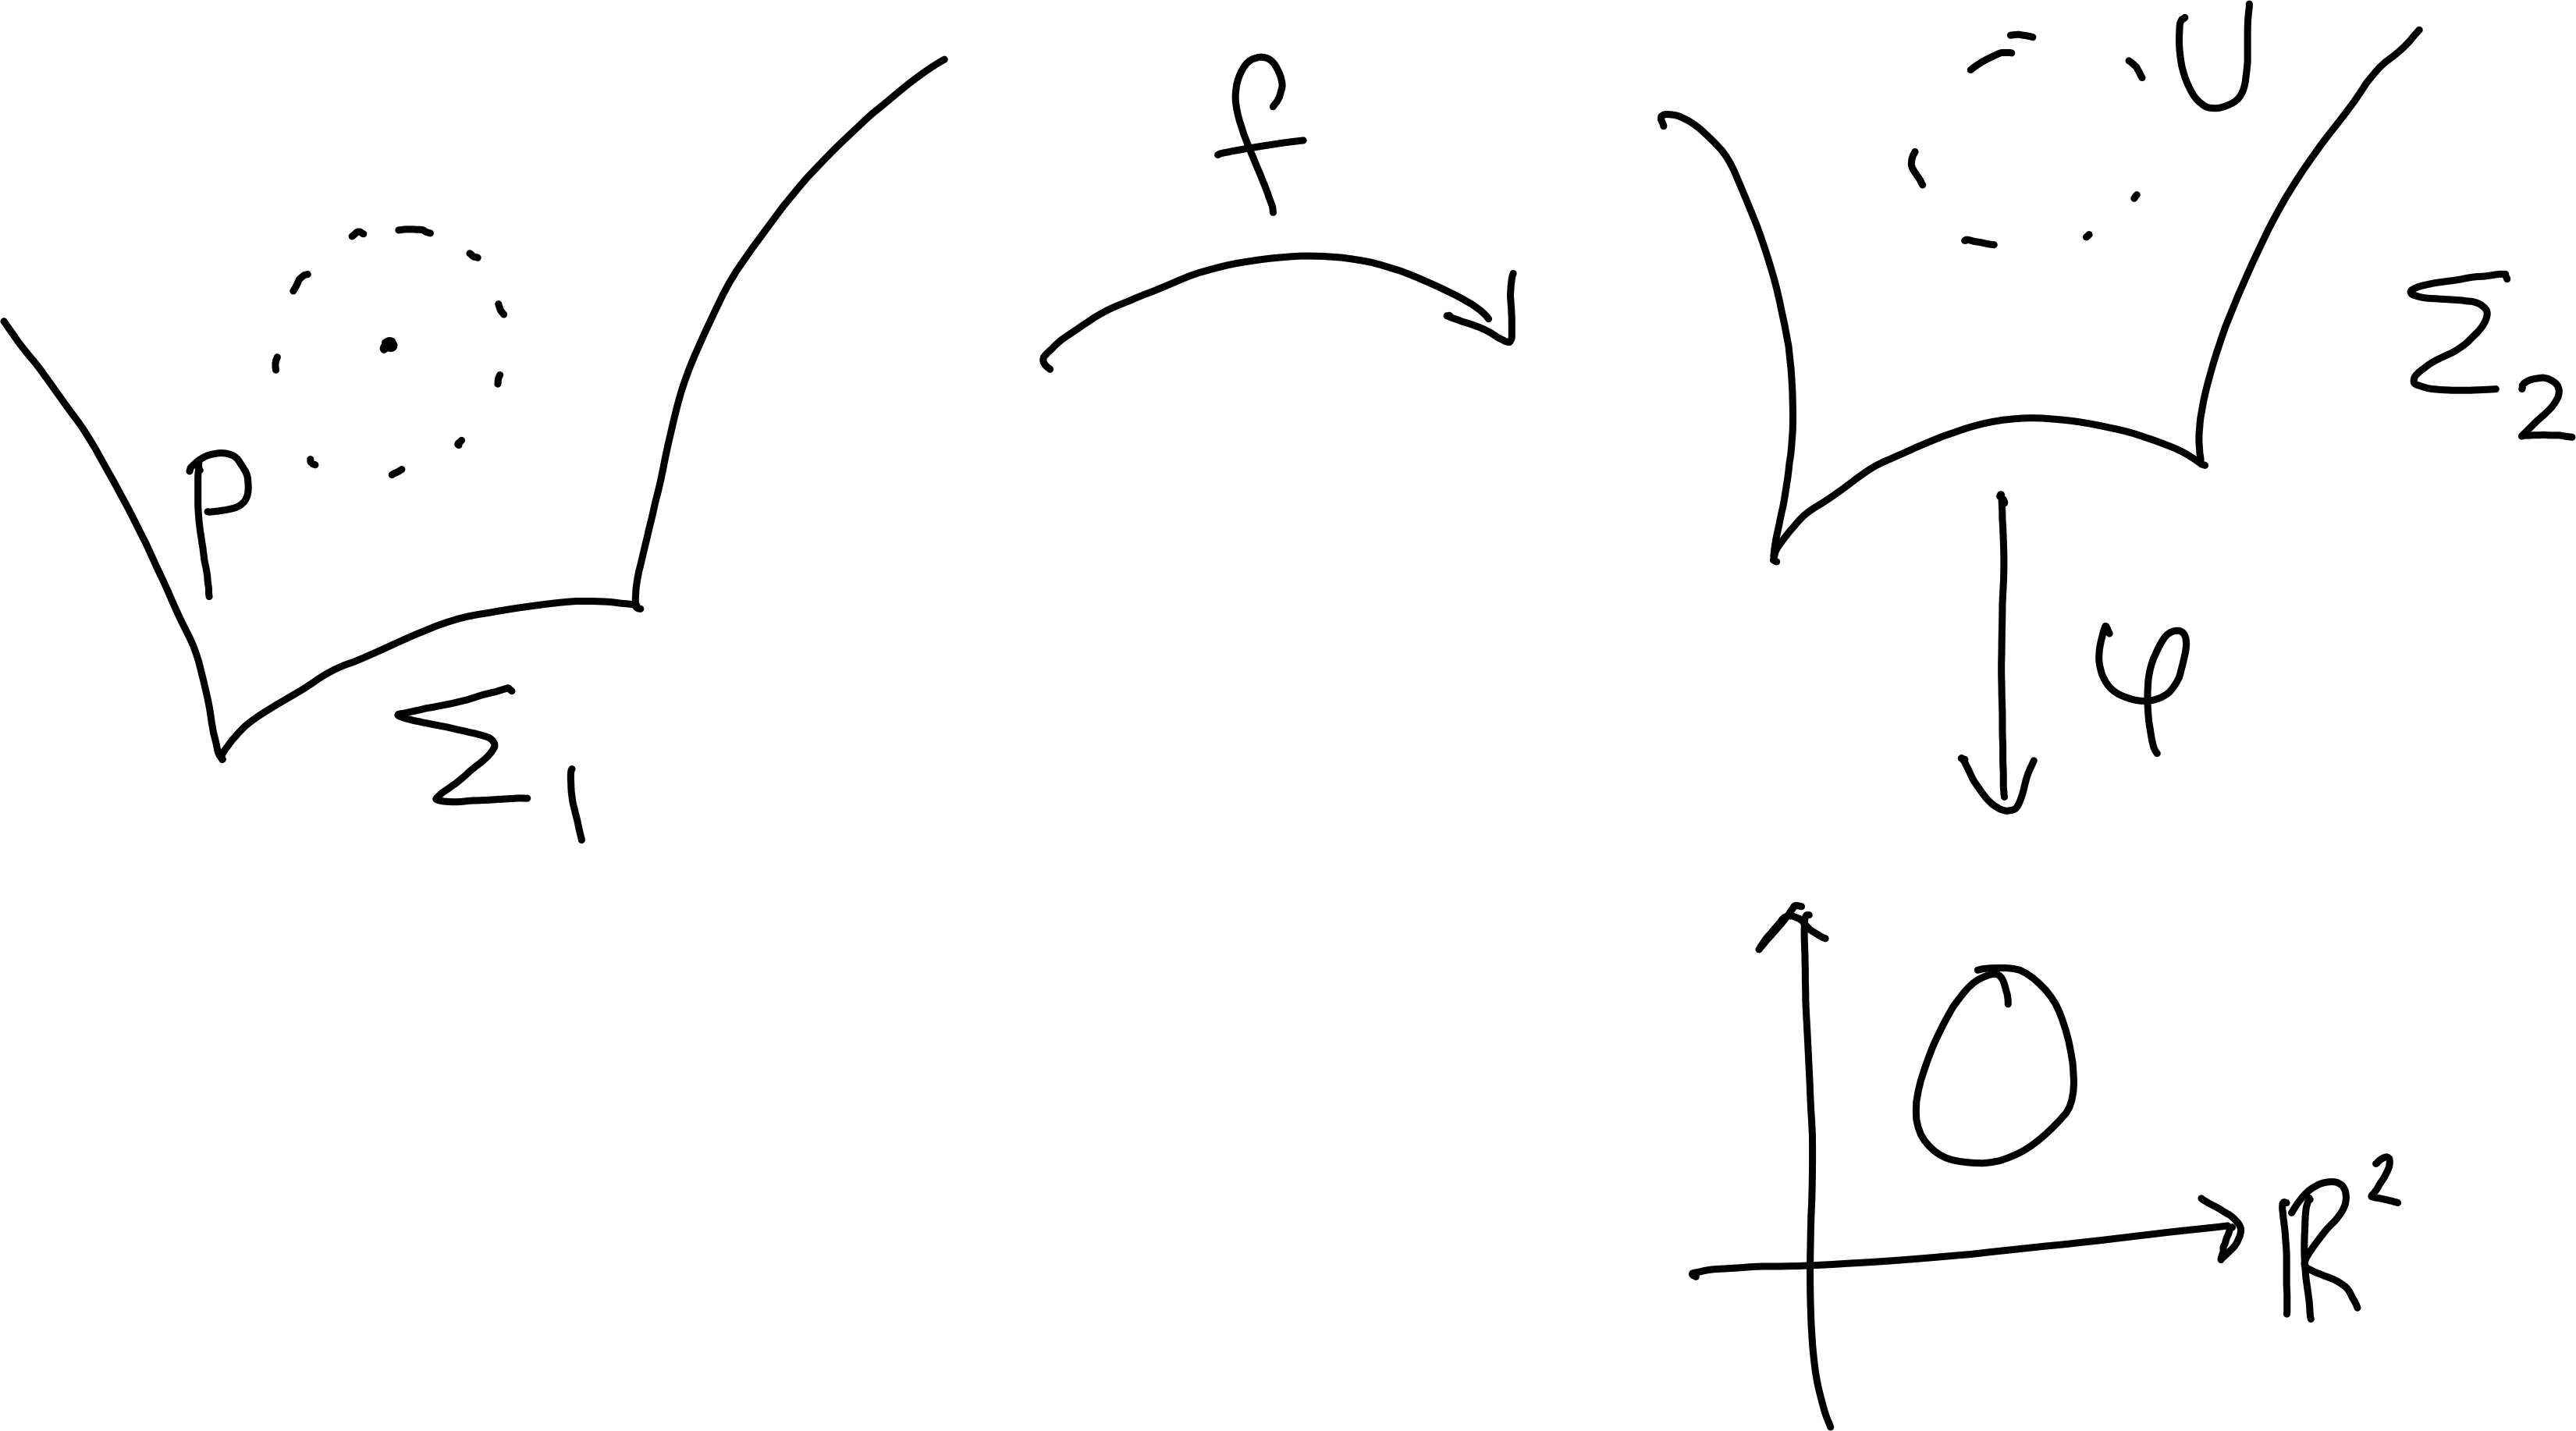
\includegraphics[height=5cm]{03-orientable} 
	\par}

	Consider the atlas on $\Sigma_1$ given by $(f^{-1}(U), \eval{\phi \circ f}_{f^{-1}(U)})$, where $(U, \psi)$ is a chart at $f(p)$ in the oriented atlas for $\Sigma_2$.
	Then, the transition function\footnote{$(\phi_1 \circ f) \circ (\phi_2 \circ f)\inv = \phi_1 \circ \phi_2\inv$} between two such charts is exactly the transition function between charts in the $\Sigma_2$ atlas.
	% In other words, in the maximal smooth atlas that exists a priori for $\Sigma_1$, we will allow charts of the form $(\widetilde U, \widetilde \psi)$ when for all charts $(U, \psi)$ at $f(p)$ in the $\Sigma_2$ atlas, the map $\psi \circ f \circ (\widetilde \psi)^{-1}$ is orientation-preserving.
	% Informally, if the atlas on $\Sigma_2$ was maximal as an oriented atlas, we can recover the previous set of charts.
\end{proof}

\begin{remark}
	\begin{enumerate}
		\item 	There is no sensible classification of the set of all smooth or topological surfaces.
		For instance, $\mathbb R^2 \setminus Z$ for a closed set $Z$ can be shown to yield uncountably many types of homeomorphisms. \\
		However, \underline{compact} smooth surfaces may be classified by their Euler characteristic and their orientability, up to diffeomorphism.
		This theorem will not be proven in this course.
		\item 	There is a definition of orientation-preserving \textit{homeomorphism} that does not rely on the determinant, but that instead relies on some algebraic topology which is not covered in this course.
		The M\"obius band is the surface
		\tikzfig{mobius_band}
		where the dashed lines represent the absence of edges.
		It is provable that an abstract smooth surface is orientable $\iff$ it contains no subsurface (an open set) homeomorphic to the M\"obius band.
		We can therefore say that a topological surface is orientable $\iff$ it contains no subsurface (an open set) homeomorphic to a M\"obius band.
		\item 	We can define other structures on an abstract smooth surface by considering smooth atlases such that if $\varphi_1 \varphi_2^{-1}$ is a transition map, then $D (\varphi_1 \varphi_2^{-1})$ at $x$ belongs to a specific subgroup $G \leq GL(2, \mathbb R)$.
		For example, defining $G = \qty{e}$ leads to Euclidean surfaces.
		The group $GL(1, \mathbb C)$ identified as a subgroup of $GL(2, \mathbb R)$ yields the Riemann surfaces, also $D (\varphi_1 \varphi_2^{-1}) \in GL(1, \mathbb C) \implies \varphi_1 \varphi_2^{-1}$ holomorphic as being in $GL(1, \mathbb C)$ implies that the Cauchy Riemann equations hold.
	\end{enumerate}
\end{remark}

\begin{example}
	For $S^2$ with the atlas of two stereographic projections, we can find the transition map to be
	\begin{align*}
		(u,v) \mapsto \qty(\frac{u}{u^2 + v^2}, \frac{v}{u^2 + v^2})
	\end{align*}
	on $\mathbb R^2 \setminus \qty{0}$.
	This has positive determinant, so $S^2$ is orientable.

	Note we only need to know the determinant at one point in $\mathbb{R}^2 \setminus \qty{0}$ as $\mathbb{R}^2 \setminus \qty{0}$ is a connected set so the determinant of the differential is a super continuous function, so if it has sign positive at one point it must have sign positive on the whole space. If its sign changed it must be $0$ somewhere but we know its a diffeomorphism so the determinant of the differential can't be 0.
\end{example}

\begin{example}
	For the torus $T^2$, we previously found an atlas such that the transition maps are translations of $\mathbb R^2$.
	Hence the torus is an oriented surface, and also a Euclidean surface.
\end{example} 

For surfaces in $\mathbb{R}^3$, we'd like to have orientability dictated by some ``ambient feature'', i.e. we want to be able to just look at the surface and know if its orientable or not.

\subsection{Tangent planes}
Recall that an \textit{affine} subspace of a vector space is a translation of a linear subspace.

\begin{definition}[Tangent Plane]
	Let $\Sigma$ be a smooth surface in $\mathbb R^3$, and $p \in \Sigma$.
	Let $\sigma \colon V \to U \subset \Sigma$ be an allowable parametrisation of $\Sigma$ near $p$, so $V$ is an open subset of $\mathbb R^2$ and $U$ is open in $\Sigma$, such that $\sigma(0) = p$.

	The \vocab{tangent plane} $T_p \Sigma$ of $\Sigma$ at $p$ is the image of $\qty(\eval{D\sigma}_0) \subset \mathbb R^3$, which is a two-dimensional vector subspace of $\mathbb R^3$.
	The \vocab{affine tangent plane} is $p + T_p \Sigma$, which is an affine subspace of $\mathbb R^3$.
\end{definition}

\begin{figure}[h] 
    \centering 
    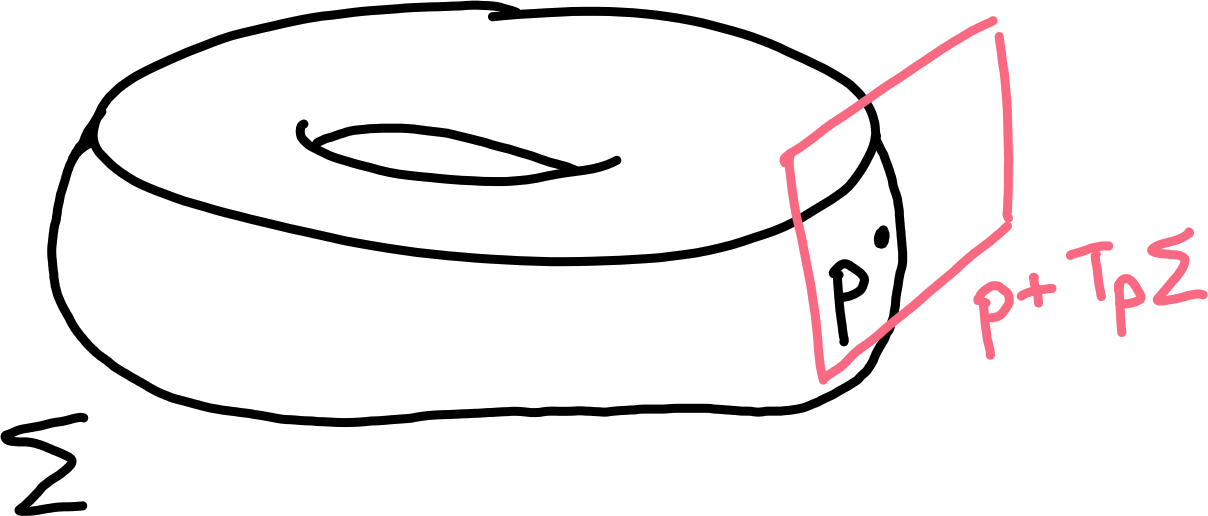
\includegraphics[height=5cm]{03-tangentplane} 
\end{figure}

\begin{remark}
	The affine tangent plane is the `best' linear approximation to a surface $\Sigma$ at a given point.
\end{remark}

\begin{lemma} \label{lem:1.9}
	$T_p \Sigma$ is well-defined, i.e. it's independent of the choice of allowable parametrisation near $p$.
\end{lemma}

\begin{proof}[Proof (i)]
	Suppose $\sigma \colon V \to U$ and $\widetilde \sigma \colon \widetilde V \to \widetilde U$ are allowable parametrisations with $\sigma(0) = \widetilde \sigma(0) = p$.
	There exists a transition map $\sigma^{-1} \circ \widetilde \sigma$, which is a diffeomorphism of open sets in $\mathbb R^2$.
	Therefore,
	\begin{align*}
		\widetilde \sigma = \sigma \circ \underbrace{\qty(\sigma^{-1} \circ \widetilde \sigma)}_{\text{diffeomorphism}}
	\end{align*}
	Hence $\eval{D(\sigma^{-1} \circ \widetilde \sigma)}_{0}$ is an isomorphism.
	Thus, the images of $D \eval{\widetilde \sigma}_0$ and $D \eval{\sigma}_0$ agree.
\end{proof}

\begin{proof}[Proof (ii)]
	Let $\gamma \colon (-\varepsilon, \varepsilon) \to \mathbb R^3$ be a smooth map such that $\gamma$ has image inside $\Sigma$, and $\gamma(0) = p$.
	We will show that $\gamma'(0) \in T_p \Sigma$.
	If $\sigma \colon V \to U$ is an allowable parametrisation with $\sigma(0) = p$ as above, and $\varepsilon$ is sufficiently small such that $\Im \gamma \subset U$, then $\gamma(t) = \sigma(u(t), v(t))$ for some smooth functions $u, v \colon (-\varepsilon, \varepsilon) \to V$.
	Then $\gamma'(t) = \sigma_u u'(t) + \sigma_v v'(t)$ is in the image of $D \eval{\sigma}_t$.
	Thus, $T_p \Sigma = \vecspan \qty{ \gamma'(0) \colon \gamma \text{ as above} }$.
\end{proof}

\begin{definition}[Normal Direction]
	If $\Sigma$ is a smooth surface in $\mathbb R^3$ and $p \in \Sigma$, the \vocab{normal direction} to $\Sigma$ at $p$ is $(T_p \Sigma)^\perp$, the Euclidean orthogonal complement to the tangent plane at $p$.
\end{definition}

\begin{remark}
	For all $p \in \Sigma$, there exist exactly two normalised normal vectors.
\end{remark}

\begin{definition}[Two-Sided]
	A smooth surface in $\mathbb R^3$ is \vocab{two-sided} if it admits a continuous global choice of unit normal vector.
\end{definition}

\begin{lemma} \label{lem:1.10}
	A smooth surface in $\mathbb R^3$ is orientable (as an abstract smooth surface) iff it is two-sided (as a smooth surface in $\mathbb R^3$).
\end{lemma}

\begin{proof}
	Let $\sigma \colon V \to U \subset \Sigma$ be an allowable parametrisation.
	Let $\sigma(0) = p$.
	We will define the positive unit normal with respect to $\sigma$ at $p$ to be the normal vector $n_\sigma(p)$ with the property that $\qty{\sigma_u, \sigma_v, n_\sigma(p)}$ and $\qty{e_1, e_2, e_3}$ are related by a positive determinant change of basis matrix (the two sets of vectors have the same orientation), where $\qty{e_1, e_2, e_3}$ are the standard basis vectors.
	In other words,
	\begin{align*}
		n_\sigma(p) = \frac{\sigma_u \times \sigma_v}{\norm{\sigma_u \times \sigma_v}}
	\end{align*}
	Consider an alternative parametrisation $\widetilde \sigma \colon \widetilde V \to \widetilde U$, where $\widetilde \sigma(0) = p$, such that $\widetilde \sigma$ belongs to the same oriented and smooth atlas as $\sigma$.
	Hence, $\sigma = \widetilde \sigma \circ \varphi$ for some transition map $\varphi = \widetilde \sigma\inv \circ \sigma$.
	Let
	\begin{align*}
		D \eval{\varphi}_0 = \begin{pmatrix}
			\alpha & \beta  \\
			\gamma & \delta
		\end{pmatrix}
	\end{align*}
	Hence,
	\begin{align*}
		\sigma_u = \alpha \widetilde \sigma_u + \gamma \widetilde \sigma_v;\quad \sigma_v = \beta \widetilde \sigma_u + \delta \widetilde \sigma_v
	\end{align*}
	This gives
	\begin{equation}
		\sigma_u \times \sigma_v = \det\qty(D \eval{\varphi}_0) \widetilde \sigma_u \times \widetilde \sigma_v \tag{$\dagger$}
	\end{equation}
	The determinant here is positive since the charts in question belong to an oriented atlas.
	Thus the positive unit normal is intrinsic to the surface, it does not depend on the choice of parametrisation.
	The expression for $n_\sigma(p)$ is continuous since the cross product is continuous, hence $\Sigma$ is two-sided.

	Conversely, if $\Sigma$ is two-sided, there exists a global continuous choice of normal vector, so we can consider the subatlas of the smooth atlas s.t we have a chart $(U,\varphi)$ with $\phi\inv = \sigma$ and $\qty{\sigma_u, \sigma_v, n}$ is an oriented basis of $\mathbb{R}^3$.
	We can make $\qty{\sigma_u, \sigma_v, n}$ have positive orientation by negating $\sigma$.
	By ($\dagger$), the transition maps between such charts are orientation-preserving.
	Hence $\Sigma$ is orientable.
\end{proof}

\begin{remark}
	Given $\gamma : (-\epsilon, \epsilon) \to \mathbb{R}^3$ smooth with $\Im(\gamma) \subset \Sigma$ and $\gamma(0) = p$.
	$\gamma(t) = \sigma(u(t), v(t))$ so $\gamma'(0) = \eval{D \sigma}_0(u'(0), v'(0)) \in T_p \Sigma$.
	This gives that $T_p \Sigma = \vecspan \qty{ \gamma'(0) \colon \gamma \text{ as above} } =$ ``tangent vectors to curves in $\Sigma$''.
\end{remark} 

\begin{lemma}
	If $\Sigma$ is a smooth surface in $\mathbb R^3$ and $A \colon \mathbb R^3 \to \mathbb R^3$ is a smooth map which preserves $\Sigma$ setwise, then $\eval{DA}_p \in L(\mathbb R^3, \mathbb R^3)$ maps $T_p \Sigma$ to $T_{A(p)} \Sigma$ for $p \in \Sigma$.
\end{lemma}

\begin{proof}
	Let $\gamma \colon (-\varepsilon, \varepsilon) \to \mathbb R^3$ be a smooth map such that its image lies on $\Sigma$, and $\gamma(0) = p$.
	Recall that $T_p \Sigma$ is spanned by $\gamma'(0)$ for such curves $\gamma$.
	Now, consider $A \circ \gamma \colon (-\varepsilon, \varepsilon) \to \mathbb R^3$, which also has image $\Sigma$, and
	\begin{align*}
		D \eval{A}_{\gamma(0)} \circ D \eval{\gamma}_0 = D \eval{A}_p \qty(\gamma'(0)) = D \eval{(A \circ \gamma)}_0 \in T_{A(p)} \Sigma
	\end{align*}
\end{proof}

\begin{example}[Unit Sphere]
	Let $S^2 \subset \mathbb{R}^3$ be the unit sphere.
	The normal vector at $p$ is the line through the origin and $p$; indeed, since $SO_3$ acts transitively on $S^2$, it suffices to check at one point, such as the north pole.
	We can choose the outward-facing normal vector to be the positive normal, denoted $n(p)$.
	$S^2$ is two-sided by the construction of this normal vector, hence $S^2$ is orientable.

	Alternatively, take any $\gamma : (-\epsilon, \epsilon) \to S^2$ with $\gamma(0) = p$.
	$\norm{\gamma(t)}^2 = 1$, so differentiating at $t = 0$, $2 \inner{\gamma'(0), p} = 0$ so $(T_p S^2)^\perp = \mathbb{R} p = \{xp: x \in \mathbb{R}\}$.
	Let $n(p) = p$, clearly a global continuous choice of normal vector so $S^2$ is 2-sided.
\end{example}

\begin{example}[M\"obius Band]
	Walk around the unit circle in the $xy$-plane and take an open interval of length 1.
	Rotate this line in the $cz$-plane as we move around the circle, s.t. it has rotated by $\frac{\theta}{2}$ after moving an angle $\theta$ in the circle (see picture).
	After a full turn the segment returns to its original position but with end points inverted. \\
	One embedding of the M\"obius band in $\mathbb R^3$ is
	\begin{align*}
		\sigma(t,\theta) = \qty(\qty(1 - t \sin \frac{\theta}{2})\cos \theta, \qty(1 - t \sin \frac{\theta}{2})\sin \theta, t \cos \frac{\theta}{2})
	\end{align*}
	where $(t,\theta) \in V_1 = \qty{t \in \qty(-\frac{1}{2}, \frac{1}{2}), \theta \in (0,2\pi)}$ or \\$(t,\theta) \in V_2 = \qty{t \in \qty(-\frac{1}{2}, \frac{1}{2}), \theta \in (-\pi, \pi)}$. \\
	This gives us the standard M\"obius band parametrically, I don't think its worthwhile trying to understand why exactly it works or what the explanation even means.

	We can check that if $\sigma_i$ is $\sigma$ on $V_i$, then $\sigma_i$ is allowable.
	Further,
	\begin{align*}
		\sigma_t \times \sigma_\theta = \qty(-\cos\theta \cos\frac{\theta}{2}, -\sin\theta \cos\frac{\theta}{2}, -\sin\frac{\theta}{2}) \equiv n_\theta
	\end{align*}
	which is already normalised.
	As $\theta \to 0$ from above, $n_\theta \to (-1,0,0)$.
	As $\theta \to 2\pi$ from below, $n_\theta \to (1,0,0)$.
	Hence, the surface is not two-sided.
\end{example}

    % \section{Geometry of surfaces in $\mathbb R^3$}

\subsection{First fundamental form}
Let $\gamma \colon (a,b) \to \mathbb R^3$ be smooth.
The \vocab{length} of $\gamma$ is
\begin{align*}
	L(\gamma) = \int_a^b \norm{\gamma'(t)} \dd{t}
\end{align*}
This result is independent of the choice of parametrisation.
Let $s \colon (A,B) \to (a,b)$ be a monotonically increasing function, let $\tau(t) = \gamma(s(t))$ and $s \geq 0$.
Then
\begin{align*}
	L(\tau) = \int_A^B \norm{\tau'(t)} \dd{t} = \int_A^B \norm{\gamma'(s(t))} \abs{s'(t)} \dd{t} = \int_a^b \norm{\gamma'(t')} \dd{s} = L(\gamma)
\end{align*}

\begin{lemma}
	If $\gamma \colon (a,b) \to \mathbb R^3$ is continuously differentiable and $\gamma'(t) \neq 0$, then $\gamma$ can be parametrised by arc length, i.e. a parameter s.t. $\norm{\gamma'(s)} = 1 \forall \; s$.
\end{lemma}

\begin{proof}
	Left as an exercise.
\end{proof} 

Let $\Sigma$ be a smooth surface in $\mathbb R^3$, and let $\sigma \colon V \to U \subset \Sigma$ be an allowable parametrisation.
If $\gamma \colon (a,b) \to U$ is smooth, then there exist functions $(u(t), v(t)) \colon (a,b) \to V$ smooth s.t. $\gamma(t) = \sigma(u(t), v(t))$.
Hence $\gamma'(t) = \sigma_u u'(t) + \sigma_v v'(t)$, giving
\begin{align*}
	\norm{\gamma'(t)}^2 = E u'(t)^2 + 2F u'(t) v'(t) + G v'(t)^2
\end{align*}
for functions
\begin{align*}
	E = \inner{\sigma_u, \sigma_u};\quad F = \inner{\sigma_u, \sigma_v} = \inner{\sigma_v, \sigma_u};\quad G = \inner{\sigma_v, \sigma_v}
\end{align*}
where $\inner{\wildcard,\wildcard}$ represents the usual Euclidean inner product.
Note that $E, F, G$ depend only on $\sigma$ and not on $\gamma$, also they are smooth functions on $V$.

\begin{definition}[First fundamental Form]
	The \vocab{first fundamental form} of $\Sigma$ in the parametrisation $\sigma$ is the expression
	\begin{align*}
		E \dd{u}^2 + 2F \dd{u} \dd{v} + G \dd{v}^2
	\end{align*}
	This notation is designed to remind you that
	\begin{align*}
		L(\gamma) = \int_a^b \sqrt{E (u')^2 + 2F u'v' + G (v')^2} \dd{t}
	\end{align*}
	where $\gamma(t) = \sigma(u(t),v(t))$.
\end{definition}

\begin{remark}
	The Euclidean inner product on $\mathbb R^3$ provides an inner product on the subspace $T_p \Sigma$.
	Choosing a parametrisation $\sigma$, we can say $T_p \Sigma = \Im D \eval{\sigma}_0 = \vecspan{\qty{\sigma_u, \sigma_v}}$ where $\sigma(0) = p$.
	The first fundamental form is a symmetric bilinear form on the tangent spaces $T_p \Sigma$, varying smoothly in $p$.
	However, we choose to express this in a basis coming from the parametrisation $\sigma$.
	In particular, we can think about the matrix expression
	\begin{align*}
		\begin{pmatrix}
			E & F \\
			F & G
		\end{pmatrix}
	\end{align*}
	This is an example of a \vocab{Riemannian metric}.
\end{remark}

\begin{example}
	The plane $\mathbb R^2_{xy} \subset \mathbb R^3$ has the parametrisation $(u,v) \mapsto (u,v,0)$.
	Hence, $\sigma_u = e_1$ and $\sigma_v = e_2$, hence the first fundamental form is $\dd{u}^2 + \dd{v}^2$.

	We could also use polar coordinates, using $\sigma(r,\theta) = (r\cos\theta,r\sin\theta,0)$.
	This parametrises the plane without the origin.
	This gives $\sigma_r = (\cos\theta,\sin\theta,0)$ and $\sigma_\theta = (-r\sin\theta, r\cos\theta,0)$.
	The first fundamental form is $\dd{r}^2 + r^2 \dd{\theta}^2$.
\end{example}

\begin{definition}[Isometries]
	Let $\Sigma, \Sigma'$ be smooth surfaces in $\mathbb R^3$.
	We say that they are \vocab{isometric} if there exists a diffeomorphism $f\colon \Sigma \to \Sigma'$ that preserves the lengths of all curves.
	More formally, for every smooth curve $\gamma \colon (a,b) \to \Sigma$, $L_\Sigma(\gamma) = L_{\Sigma'}(f \circ \gamma)$.
\end{definition}

\begin{example}
	Let $\Sigma' = f(\Sigma)$ where $f \colon \mathbb R^3 \to \mathbb R^3$ is a global isometry, or rigid motion, of $\mathbb R^3$; that is, $v \mapsto Av+b$ for an orthogonal matrix $A$.
	These isometries preserve the Euclidean inner product on $\mathbb R^3$, hence $f$ preserves length and so it is an isometry.
	\begin{align*}
	   \norm{(f \circ \gamma)'(t)} &= \norm{A \gamma'(t)} \\
	   &= \norm{\gamma'(t)}.  
	\end{align*} 
	However, in the definition, we need not map all of $\mathbb R^3$ to itself, just $\Sigma \to \Sigma'$.
\end{example}

Often we're interested in local statements.

\begin{definition}[Locally Isometric]
	We say that $\Sigma$ and $\Sigma'$ are \vocab{locally isometric} near points $p \in \Sigma$ and $q \in \Sigma'$ if there exist open neighbourhoods $U$ of $p$ and $V$ of $q$ such that $U$ and $V$ are isometric.
\end{definition}

We can also say that $\Sigma$ and $\Sigma'$ are locally isometric if they are locally isometric at all points; that is, each point of $\Sigma$ is locally isometric to some point on $\Sigma'$.

\begin{lemma}
	Smooth surfaces $\Sigma, \Sigma'$ in $\mathbb R^3$ are locally isometric near $p \in \Sigma$ and $q \in \Sigma'$ iff there exist allowable parametrisations $\sigma \colon V \to U \subset \Sigma$ and $\sigma' \colon V \to U' \subset \Sigma'$ such that the first fundamental forms are equal in $V$ ($E = E', F = F', G = G'$).
\end{lemma}

\begin{figure}[h] 
    \centering 
    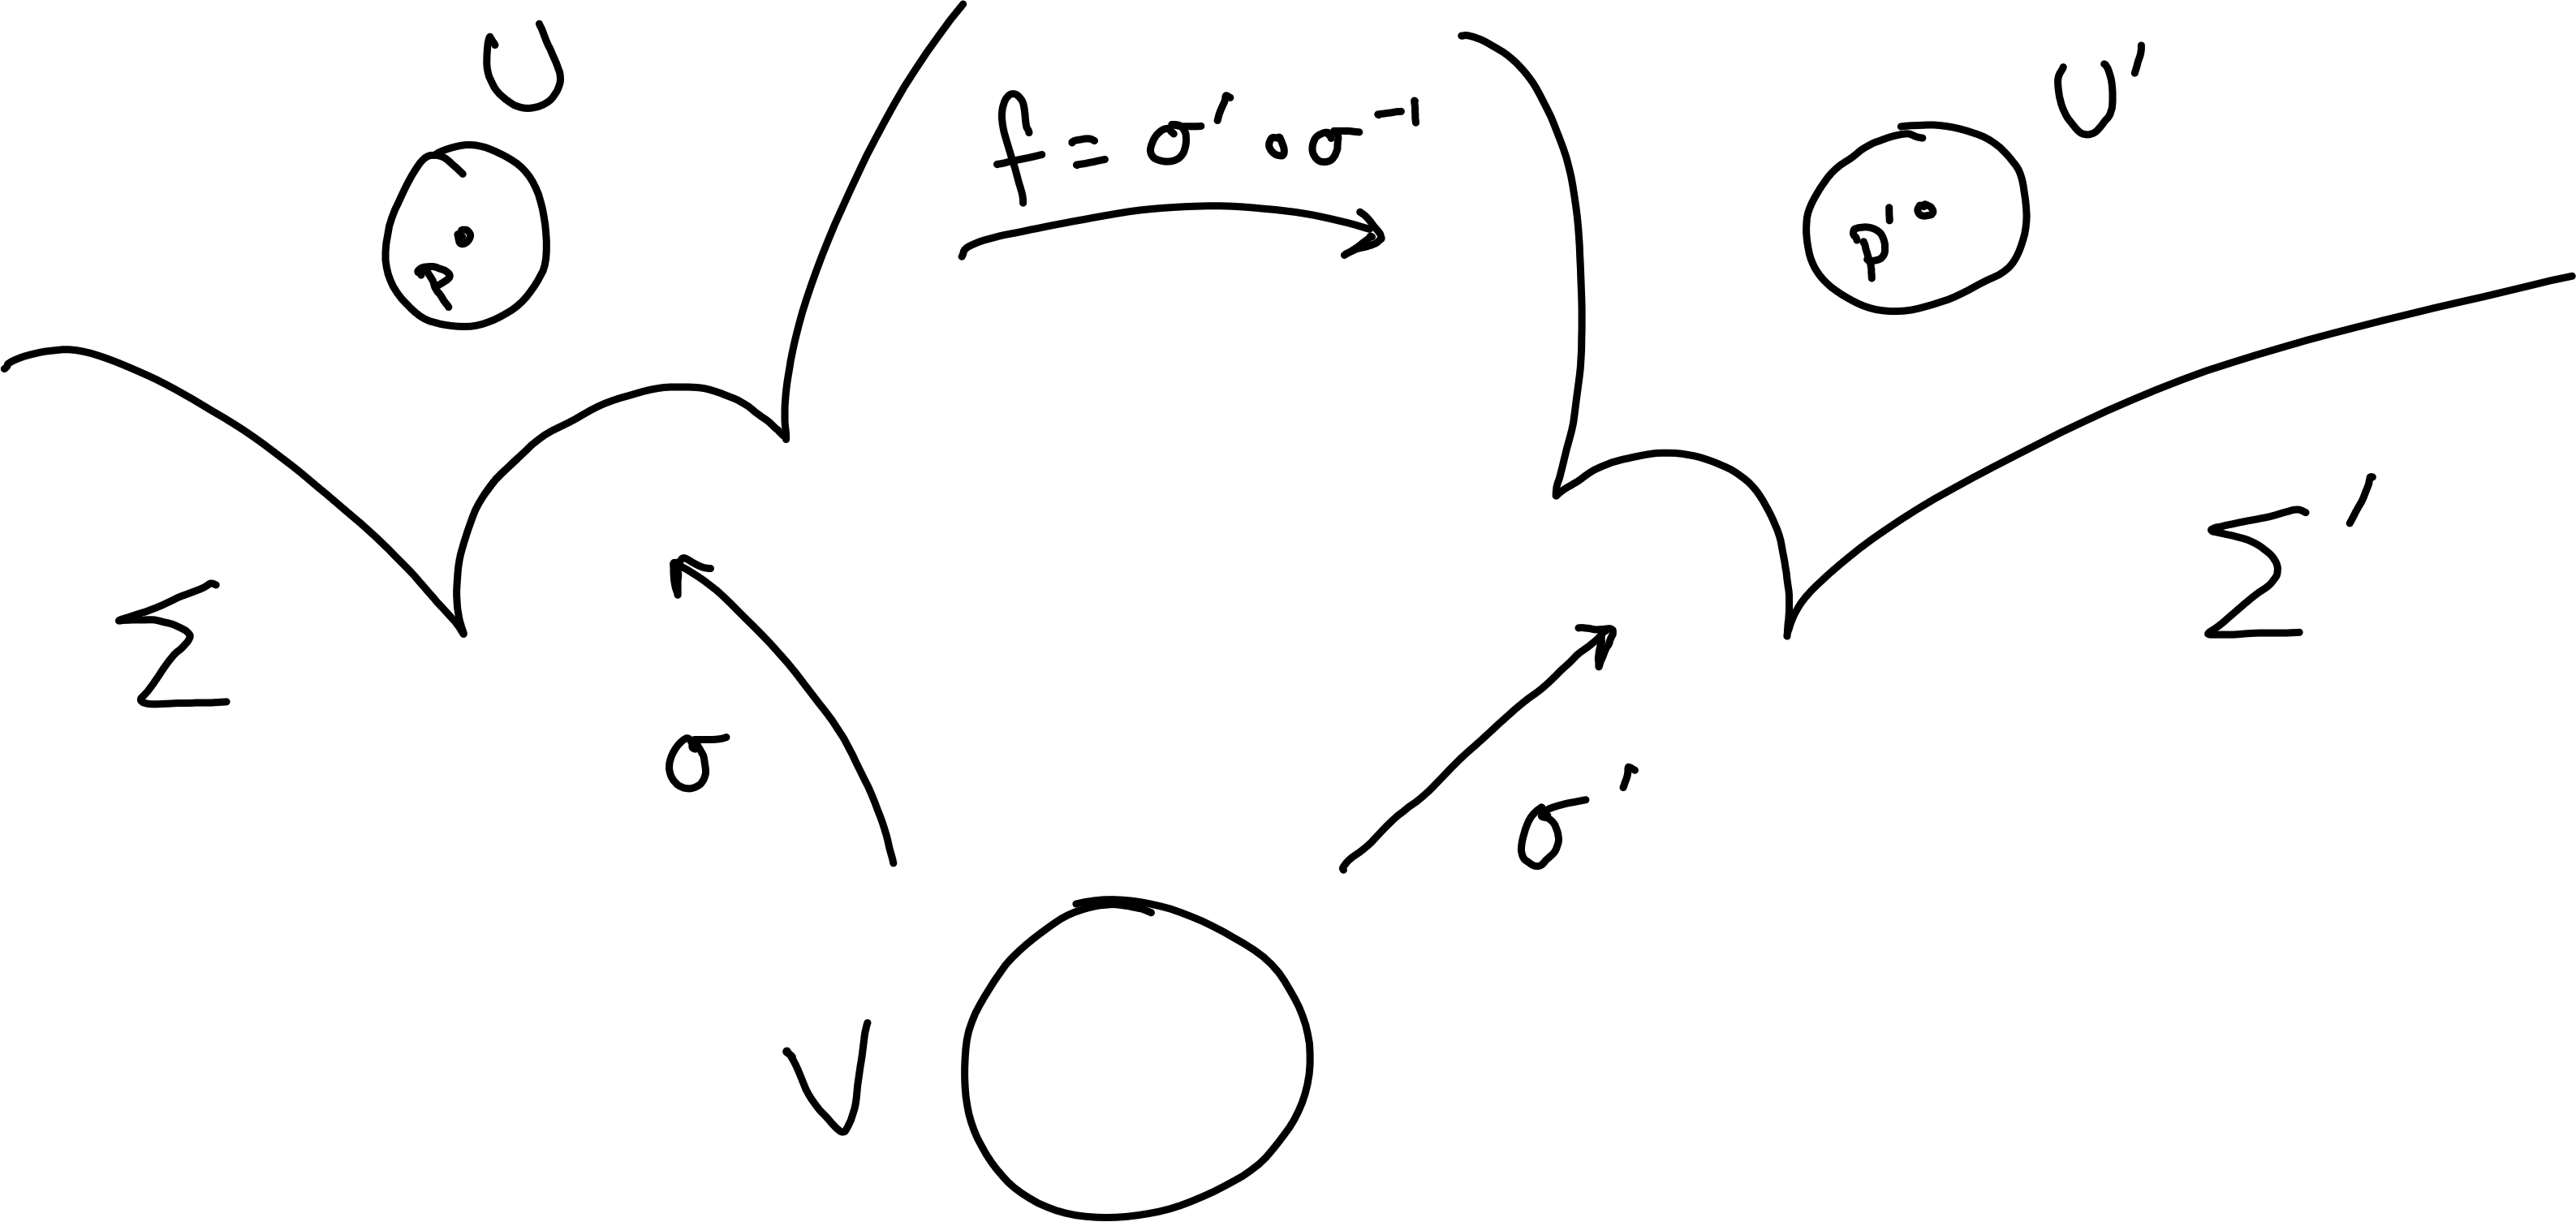
\includegraphics[height=5cm]{04-locallyIsometric} 
\end{figure}

\begin{proof}
	By definition, the first fundamental form of $\Sigma$ determines the lengths of all curves on $\Sigma$ that lie in $\sigma(V) = U$.

	$(\Longleftarrow)$: If we have $\sigma$ and $\sigma'$ with equal fundamental forms, then $\sigma' \circ \sigma\inv : U \to U'$ is an isometry since given curve $\gamma(t)$
	\begin{align*}
		\sigma\inv(\gamma(t)) &= (u(t), v(t)) \\
		\norm{\frac{d}{dt} \underbracket{\sigma' \circ \sigma\inv}_f \circ \gamma}^2 &= \norm{\frac{d}{dt} \sigma'(u(t), v(t))}^2 \\
		&= E' \dot{u}^2 + 2 F' \dot{u} \dot{v} + G' \dot{v}^2 \\
		&= E \dot{u}^2 + 2 F \dot{u} \dot{v} + G \dot{v}^2 \\
		&= \norm{\frac{d}{dt} \gamma(t)}^2 \\
		\therefore L(\sigma' \circ \sigma\inv \circ \gamma) &= L(\gamma).
	\end{align*} 

	$(\implies)$: We shall first show that the lengths of curves in $U$ determine the first fundamental form of $\sigma$.
	Given $\sigma \colon V \to U$, without loss of generality let $V = B(0,\delta)$ for some $\delta > 0$, where $\sigma(0) = p$.
	Consider, for all $\varepsilon < \delta$, the curve
	\begin{align*}
		\gamma_\varepsilon \colon [0,\varepsilon] \to U;\quad t \mapsto \sigma(t,0)
	\end{align*}
	Then,
	\begin{align*}
		\dv{\varepsilon} L(\gamma_\varepsilon) = \dv{\varepsilon} \int_0^\varepsilon \sqrt{E(t,0)} \dd{t} = \sqrt{E(\varepsilon,0)}
	\end{align*}
	Hence,
	\begin{align*}
		\eval{\dv{\varepsilon}}_{\varepsilon = 0} L(\gamma_\varepsilon) = \sqrt{E(0,0)}
	\end{align*}
	So we can determine $E$ at $p$ by looking at lengths of curves.
	We can similarly consider
	\begin{align*}
		\chi_\varepsilon \colon [0,\varepsilon] \to U;\quad t \mapsto \sigma(0,t)
	\end{align*}
	which determines $G$.
	Finally, consider
	\begin{align*}
		\lambda_\varepsilon \colon [0,\varepsilon] \to U;\quad t \mapsto \sigma(t,t)
	\end{align*}
	which determines $\sqrt{(E+2F+G)(0,0)}$ which gives $F$ implicitly.

	So if $f: U \to U'$ is a local isometry take any allowable parametrisation $\sigma' : V \to U'$ then $ = f\inv \circ \sigma'$ is s.t. the first fundamental form of $\sigma, \sigma'$ agree.
\end{proof}

\begin{example}
	Consider the cone with angle $\arctan a$ to the vertical.
	{\par
		\centering 
		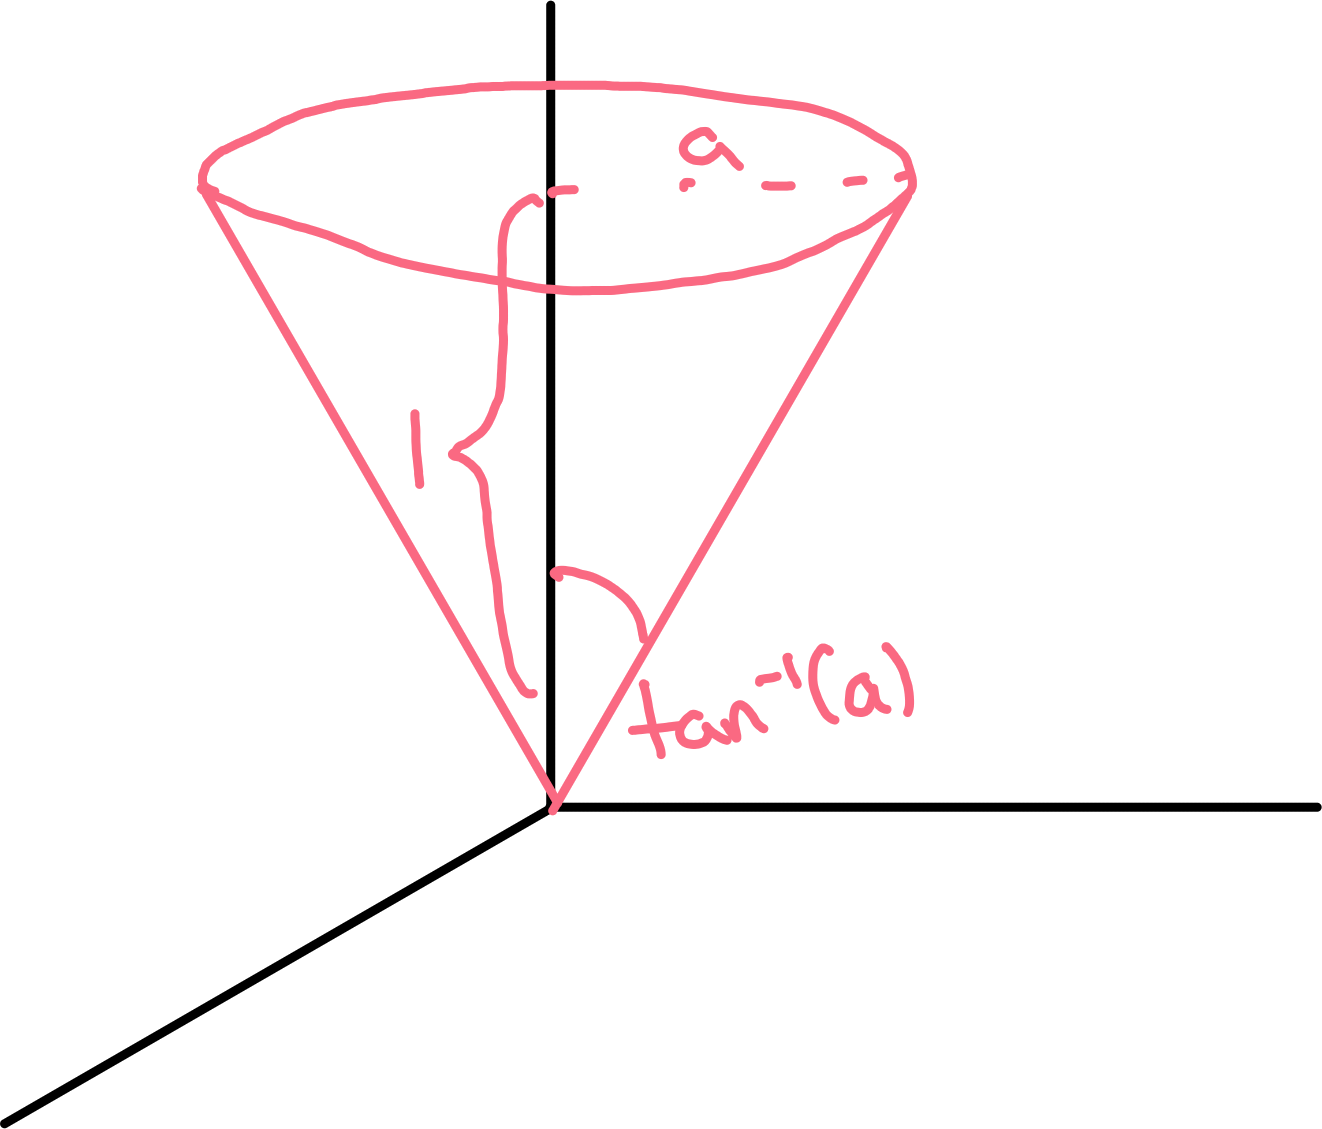
\includegraphics[height=5cm]{04-cone} 
	\par}
	For $u > 0$ and $v \in (0,2\pi)$, we define
	\begin{align*}
		\sigma(u,v) = (au\cos v, au\sin v, u).
	\end{align*}
	This parametrises the cone excluding the line at $v = 0$. \\
	The first fundamental form is
	\begin{align*}
		(1+a^2)\dd{u}^2 + a^2 u^2 \dd{v}^2
	\end{align*}
	Consider cutting the cone along the line $v = 0$ and flattening it into a plane sector.
	{\par
		\centering 
		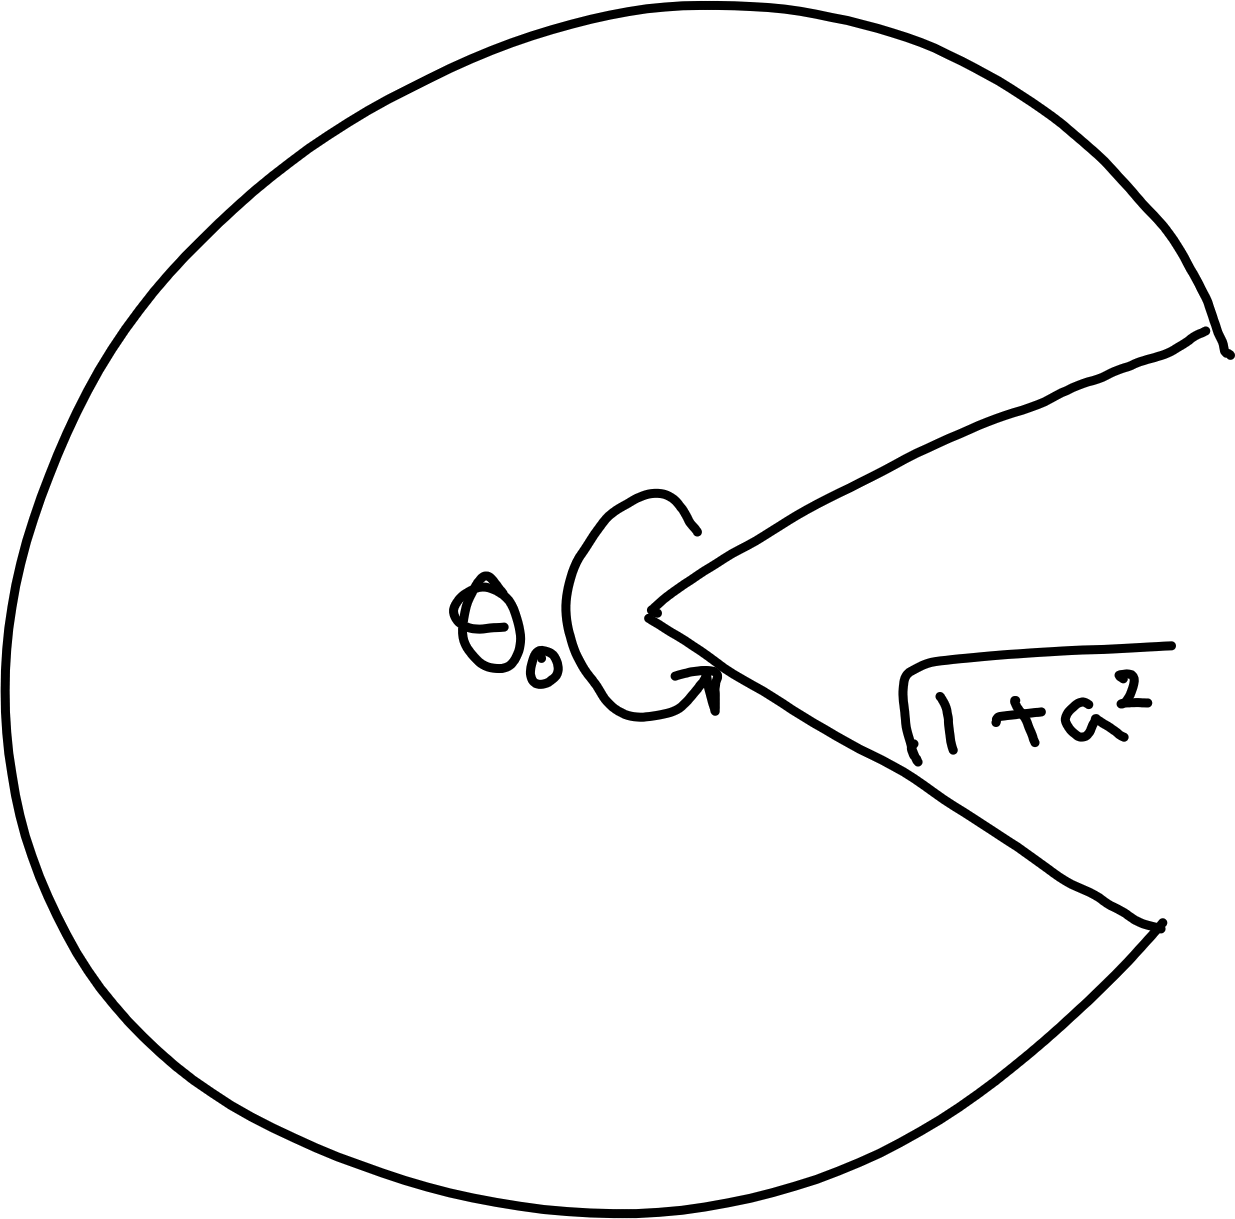
\includegraphics[height=5cm]{04-cone-unrolled} 
	\par}
	The circumference of the sector is $2 \pi a$ and the radius is $\sqrt{1+a^2}$, hence the angle traced out by the sector is $\theta_0 = \frac{2 \pi a}{\sqrt{1+a^2}}$.
	We can parametrise this subset of the plane by
	\begin{align*}
		\sigma(r,\theta) = \qty(\sqrt{1+a^2} r\cos\qty(\frac{a\theta}{\sqrt{1+a^2}}), \sqrt{1+a^2} r\sin\qty(\frac{a\theta}{\sqrt{1+a^2}}), 0)
	\end{align*}
	for $r > 0$ and $\theta \in (0,2\pi)$.
	We can then check that the first fundamental form here is
	\begin{align*}
		(1+a^2) \dd{r}^2 + r^2 a^2 \dd{\theta}^2
	\end{align*}
	which matches the first fundamental form for the cone itself.
	Hence the cone and the plane are locally isometric.

	However, the cone and plane are not globally isometric, since the two topological spaces are not homeomorphic, so no diffeomorphism that preserves lengths can be constructed.
	An intuitive way to think about this is that the cone doesn't include the origin so shrinking any curve on the cone to $0$ leaves the cone whilst the same is not true in the plane, this is the notion of simple connectedness.
\end{example}

\begin{example}
	The sphere of radius $a$, given by $\qty{x^2 + y^2 + z^2 = a^2}$, has an open set with allowable parametrisation
	\begin{align*}
		\sigma(u,v) = (a\cos u \cos v, a \cos u \sin v, a \sin u)
	\end{align*}
	where $u \in \qty(-\frac{\pi}{2}, \frac{\pi}{2})$ and $v \in (0,2\pi)$.
	This parametrises the complement of a half great circle.
	Here,
	\begin{align*}
		\sigma_u = (-a \sin u \cos v, -a \sin u \sin v, a \cos u);\quad \sigma_v = (-a \cos u \sin v, a \cos u \cos v, 0)
	\end{align*}
	Hence,
	\begin{align*}
		E = a^2; \quad F = 0;\quad G = a^2 \cos^2 u
	\end{align*}
	which gives the first fundamental form as
	\begin{align*}
		a^2 \dd{u}^2 + a^2 \cos^2 u \dd{v}^2
	\end{align*}
\end{example}

\begin{example}
	Consider the surface of revolution given by a curve
	\begin{align*}
		\eta(t) = (f(t),0,g(t))
	\end{align*}
	rotated about the $z$ axis.
	The resulting surface has parametrisation
	\begin{align*}
		\sigma(u,v) = (f(u) \cos v, f(u) \sin v, g(u))
	\end{align*}
	Hence,
	\begin{align*}
		\sigma_u = (f_u \cos v, f_u \sin v, g_u);\quad \sigma_v = (-f \sin v, f \cos v, 0)
	\end{align*}
	which gives
	\begin{align*}
		(f_u^2 + g_u^2) \dd{u}^2 + f^2 \dd{v}^2
	\end{align*}
\end{example}

\begin{lemma} \label{lem:2.3}
	Let $\Sigma$ be a smooth surface in $\mathbb R^3$, and let $p \in \Sigma$.
	Suppose we have two allowable parametrisations $\sigma \colon V \to U$ and $\sigma' \colon V' \to U$ s.t. $\sigma(0) = \sigma'(0) = p$ and U an open nbd of $p$.
	The two parametrisations differ by a transition map $f = {\sigma'}^{-1} \circ \sigma$ which is a diffeomorphism of open subsets of $\mathbb R^2$.
	There exist first fundamental forms for both parametrisations.
	Then,
	\begin{align*}
		\begin{pmatrix}
			E & F \\
			F & G
		\end{pmatrix} = (Df)^\tran \begin{pmatrix}
			E' & F' \\
			F' & G'
		\end{pmatrix} (Df)
	\end{align*}
\end{lemma}

\begin{proof}
	By definition,
	\begin{align*}
		\begin{pmatrix}
			E & F \\
			F & G
		\end{pmatrix} = \begin{pmatrix}
			\sigma_u \cdot \sigma_u & \sigma_u \cdot \sigma_v \\
			\sigma_v \cdot \sigma_u & \sigma_v \cdot \sigma_v
		\end{pmatrix} = (D\sigma)^\tran (D\sigma)
	\end{align*}
	Since, $\sigma = \sigma' \circ F \implies D \sigma = D \sigma' Df$ so $(D\sigma)^\tran (D\sigma) = (D \sigma = D \sigma' Df)^\tran (D \sigma = D \sigma' Df) = (Df)^\tran (D\sigma')^\tran (D\sigma') (Df)$.
\end{proof}

\subsection{Conformality}
If $v,w \in \mathbb R^3$, we have $v \cdot w = \norm{v} \cdot \norm{w} \cdot \cos\theta$.
This allows us to deduce the angle $\theta$ between two vectors given their dot product and lengths.
This can also be done when $v,w$ are in the tangent plane $T_p \Sigma$, and then we can express the angle in terms of the first fundamental form.
Let $\sigma$ be an allowable parametrisation for $\Sigma$ near $p$, such that $D\eval{\sigma}_0$ evaluates to $v$ at $v_0$ and $w$ at $w_0$.
\begin{align*}
	\cos \theta &= \frac{v \cdot w}{\norm{v} \cdot \norm{w}} = \frac{I(v_0, w_0)}{\sqrt{I(v_0,v_0)} \sqrt{I(w_0,w_0)}} \\
	I(v_0, w_0) &= v_0^\tran \begin{pmatrix}
		E & F \\
		F & G
	\end{pmatrix} w_0.
\end{align*}
where $I$ denotes the first fundamental form of $\sigma$ at zero.

\begin{lemma}
	Let $\Sigma$ be a smooth surface in $\mathbb R^3$, and let $\sigma \colon V \to U$ be an allowable parametrisation of $\Sigma$ near $p$. \\
	Then $\sigma$ is \textit{conformal} (preserves angles) iff $E = G$ and $F = 0$ in the first fundamental form.
\end{lemma}

\begin{proof}
	$(\implies)$: Consider curves $\gamma \colon t \mapsto (u(t), v(t))$ and $\widetilde \gamma \colon t \mapsto (\widetilde u(t), \widetilde v(t))$ in $V$, where $\gamma(0) = \widetilde \gamma(0) = 0 \in V$.
	Let $\sigma$ be a parametrisation $V \to U \subset \Sigma$ such that $\sigma(0) = p \in \Sigma$.
	Then the curves $\sigma \circ \gamma$ and $\sigma \circ \widetilde \gamma$ meet at angle $\theta$ on $\Sigma$, where
	\begin{align*}
		\cos \theta = \frac{E \dot u \dot {\widetilde u} + F \qty(\dot u \dot{\widetilde v} + \dot v \dot{\widetilde u}) + G \dot v \dot{\widetilde v}}{\sqrt{E \dot u^2 + 2F \dot u \dot v + G \dot v^2} \sqrt{E \dot{\widetilde u}^2 + 2F \dot{\widetilde u} \dot {\widetilde v} + G \dot{\widetilde v}^2}}
	\end{align*}
	In particular, if $\sigma$ is conformal, suppose $\gamma(t) = (t,0)$ and $\widetilde \gamma(t) = (0,t)$.
	Then, we have that the curves meet at $\frac{\pi}{2}$ in $V$, so they meet at $\frac{\pi}{2}$ in $\Sigma$, so we find that $\cos \theta = 0 \implies F = 0$ as $\dot{u} = \dot{\widetilde v} = 1$ and $\dot{\widetilde u} = \dot{v} = 0$. \\
	Similarly, if $\gamma(t) = (t,t)$ and $\widetilde \gamma(t) = (t,-t)$, we find $\cos \theta = 0 \implies E = G$.

	$(\Longleftarrow)$: Conversely, suppose there exists a parametrisation $\sigma$ such that $E = G$ and $F = 0$.
	Then, in this parametrisation, the first fundamental form is of the form $\rho \qty(\dd{u}^2 + \dd{v}^2)$ for $\rho = E \colon V \to \mathbb R$.
	So \begin{align*}
		\cos \theta = \frac{\dot u \dot {\widetilde u} + \dot v \dot{\widetilde v}}{\sqrt{\dot u^2 + \dot v^2} \sqrt{\dot{\widetilde u}^2 + \dot{\widetilde v}^2}},
	\end{align*} i.e. angles don't change.

	Alternatively, the first fundamental form is a pointwise rescaling of the Euclidean fundamental form $\dd{u}^2 + \dd{v}^2$.
	Rescaling the plane does not change angles, so $\sigma$ is conformal as required.
\end{proof}

\begin{remark}
	Conformality in charts is historically important for cartography.
	The existence of conformal charts is closely connected to Riemann surfaces, which are topological surfaces locally modelled on $\mathbb C$ instead of $\mathbb R^2$.
\end{remark}

\subsection{Area}
Recall that a parallelogram spanned by vectors $v, w$ has area \\$\norm{v \times w} = \sqrt{\inner{v,v}\inner{w,w} - \inner{v,w}^2}$, where $\times$ denotes the cross product.
Let $\sigma \colon V \to U \subset \Sigma$ be an allowable parametrisation with $\sigma(0) = p$, and consider $\sigma_u, \sigma_v \in T_p \Sigma$.
The square of the area of the infinitesimal parallelogram spanned by $\sigma_u, \sigma_v$ is given by
\begin{align*}
	\qty(\inner{\sigma_u, \sigma_u}\inner{\sigma_v, \sigma_v} - \inner{\sigma_u, \sigma_v}^2)^{1 / 2} = \sqrt{EG - F^2}.
\end{align*}

\begin{definition}[Area]
	Let $\Sigma$ be a smooth surface in $\mathbb R^3$, and $\sigma \colon V \to U \subset \Sigma$ an allowable parametrisation.
	Then,
	\begin{align*}
		\mathrm{area}(U) = \int_V \sqrt{EG - F^2} \dd{u}\dd{v}
	\end{align*}
\end{definition}

\begin{remark}
	This is independent of parametrisation.
	Indeed, suppose $\sigma \colon V \to U$ and $\widetilde \sigma \colon \widetilde V \to U$ are allowable.
	Then $\widetilde \sigma = \sigma \circ \varphi$ for some transition map $\varphi = \sigma\inv \circ \widetilde \sigma \colon \widetilde V \to V$.
	We know then that by \Cref{lem:2.3}
	\begin{align*}
		\begin{pmatrix}
			\widetilde E & \widetilde F \\
			\widetilde F & \widetilde G
		\end{pmatrix} = (D\widetilde \sigma)^\tran (D\widetilde \sigma) = (D\varphi)^\tran \begin{pmatrix}
			E & F \\
			F & G
		\end{pmatrix} (D\varphi)
	\end{align*}
	Hence by taking determinants,
	\begin{align*}
		\sqrt{\widetilde E \widetilde G - \widetilde F^2} = \abs{\det(D\varphi)} \sqrt{EG - F^2}
	\end{align*}
	The usual change of variables formula for integration, combined with the fact that $\varphi$ is a diffeomorphism, gives
	\begin{align*}
		\int_V \sqrt{EG - F^2} \dd{u}\dd{v} = \int_{\widetilde V} \sqrt{\widetilde E \widetilde G - \widetilde F^2} \dd{\widetilde u}\dd{\widetilde v}.
	\end{align*}
	So $\operatorname{area}(U)$ is intrinsic and well-defined.

	Note, we can compute the area of an open set $U \subset \Sigma$, not necessarily lying in a single parametrisation, by covering the set by a finite amount of open subsets which lie in single charts.
	For instance, if $\Sigma$ is compact, we can compute the area of $\Sigma$ itself.
\end{remark}

\begin{example}
	Consider the graph $\Sigma = \qty{(u,v,f(u,v)) \colon (u,v) \in \mathbb R^2}$, where $f \colon \mathbb R^2 \to \mathbb R$ is a smooth function.
	This has a global parametrisation $\sigma(u,v) = (u,v,f(u,v))$.
	Here, $\sigma_u = (1,0,f_u)$ and $\sigma_v = (0,1,f_v)$, hence
	\begin{align*}
		\sqrt{EG - F^2} = \sqrt{1+f_u^2+f_v^2}
	\end{align*}
	Let $U_R \subset \Sigma$ be the part of the graph lying inside the disc $B(0,R) \subset \mathbb R^2$.
	Then
	\begin{align*}
		\mathrm{area}(U_R) = \int_{B(0,R)} \sqrt{1+f_u^2+f_v^2} \dd{u}\dd{v} \geq \pi R^2
	\end{align*}
	with equality exactly when $f_u = f_v = 0$, which is when $f$ is constant and $U_R$ is contained inside a plane perpendicular to the $z$ axis.
	Hence, the projection from $\Sigma$ to $\mathbb R^2_{xy}$ is not area-preserving, unless $\Sigma$ is a plane perpendicular to the $z$ axis.
\end{example}

\begin{example}
	Consider the sphere enclosed exactly by a cylinder.
	The cylindrically radial projection from the sphere to the cylinder is area-preserving.
	You will prove this in Sheet 2.
\end{example}

\subsection{Second fundamental form}
Let $\sigma \colon V \to U \subset \Sigma$ be allowable.
By using Taylor's theorem, we can write
\begin{align*}
	\sigma(u+h,v+\ell) = \sigma(u,v) + h \sigma_u(u,v) + \ell \sigma_v(u,v) + \frac{1}{2} \qty(h^2 \sigma_{uu}(u,v) + 2h\ell \sigma_{uv}(u,v) + \ell^2 \sigma_{vv}(u,v)) + O(h^3,\ell^3)
\end{align*}
where $h,\ell$ are small, and $(u+h,v+\ell) \in V$.
Recall that if $p = \sigma(u,v)$, we have $T_p \Sigma = \genset{\qty{\sigma_u,\sigma_v}}$.
Hence, the orthogonal distance from $\sigma(u+h,v+\ell)$ to the affine tangent plane $T_p \Sigma + p$ is given by projection to the normal direction.
\begin{align*}
	\inner{n,\sigma(u+h,v+\ell) - \sigma(u,v)} = \frac{1}{2} \qty(\inner{n,\sigma_{uu}} h^2 + 2\inner{n,\sigma_{uv}} h\ell + \inner{n,\sigma_{vv}}\ell^2) + O(h^3,\ell^3)
\end{align*}
\begin{definition}
	The \textit{second fundamental form} of $\Sigma$ in the allowable parametrisation $\sigma$ is the quadratic form
	\begin{align*}
		L \dd{u}^2 + 2 M \dd{u} \dd{v} + N \dd{v}^2
	\end{align*}
	where
	\begin{align*}
		L = \inner{n,\sigma_{uu}};\quad M = \inner{n,\sigma_{uv}};\quad N = \inner{n,\sigma_{vv}}
	\end{align*}
	and
	\begin{align*}
		n = \frac{\sigma_u \times \sigma_v}{\norm{\sigma_u \times \sigma_v}}
	\end{align*}
	We can write this as the matrix
	\begin{align*}
		\begin{pmatrix}
			L & M \\
			M & N
		\end{pmatrix}
	\end{align*}
	which defined a quadratic form on $T_p \Sigma$ which varies smoothly in $p$.
\end{definition}
\begin{lemma}
	Let $V$ be connected and $\sigma \colon V \to U \subset \Sigma$ be an allowable parametrisation such that the second fundamental form vanishes identically with respect to $\sigma$.
	Then $U$ lies in an affine plane.
\end{lemma}
\begin{remark}
	The first fundamental form is a non-degenerate symmetric bilinear form on $T_p \Sigma$, whereas the second fundamental form may be degenerate.
\end{remark}
\begin{proof}
	By definition,
	\begin{align*}
		\inner{n,\sigma_u} = 0 = \inner{n,\sigma_v}
	\end{align*}
	Hence, by differentiating, we find
	\begin{align*}
		0 = \inner{n_u, \sigma_u} + \inner{n, \sigma_{uu}} = \inner{n_v, \sigma_v} + \inner{n, \sigma_{vv}} = \inner{n_v, \sigma_u} + \inner{n,\sigma_{uv}}
	\end{align*}
	Some of these terms appear in the definition of the second fundamental form:
	\begin{align*}
		L = \inner{n,\sigma_{uu}} = -\inner{n_u, \sigma_u};\quad M = \inner{n,\sigma_{uv}} = -\inner{n_v, \sigma_u} = -\inner{n_u, \sigma_v};\quad N = \inner{n,\sigma_{vv}} = -\inner{n_v, \sigma_v}
	\end{align*}
	If the second fundamental form vanishes, then $n_u$ is orthogonal to $\sigma_u$, $\sigma_v$, and $n$ itself.
	Since $\sigma_u, \sigma_v, n$ form a basis for $\mathbb R^3$, we have $n_u = 0$.
	Similarly, $n_v = 0$, hence $n$ is constant by the mean value theorem.
\end{proof}
\begin{remark}
	The first fundamental form in parametrisation $\sigma$ can be written $(D \sigma)^\tran (D \sigma)$.
	We can similarly write the second fundamental form as
	\begin{align*}
		-(Dn)^\tran (D\sigma) = \begin{pmatrix}
			L & M \\
			M & N
		\end{pmatrix} = -\begin{pmatrix}
			n_u \cdot \sigma_u & n_u \cdot \sigma_v \\
			n_v \cdot \sigma_u & n_v \cdot \sigma_v
		\end{pmatrix}
	\end{align*}
	Hence, if $\sigma \colon V \to \Sigma$ and $\widetilde \sigma \colon \widetilde V \to \Sigma$ are allowable parametrisations for an open set $U \subset \Sigma$ with transition map $\varphi \colon \widetilde V \to V$ given by $\varphi = \sigma^{-1} \circ \widetilde \sigma$, we can use the above expression to find
	\begin{align*}
		\begin{pmatrix}
			\widetilde L & \widetilde M \\
			\widetilde M & \widetilde N
		\end{pmatrix} = \pm (D\varphi)^\tran \begin{pmatrix}
			L & M \\
			M & N
		\end{pmatrix} (D\varphi)
	\end{align*}
	The change in sign depends on whether the transition map preserves or reverses orientation.
	If the normal vectors agree, there is no negative sign.
	\begin{align*}
		\eval{n_{\sigma \circ \varphi}}_{(\widetilde u, \widetilde v)} = \pm \eval{n_\sigma}_{\varphi(\widetilde u, \widetilde v)}
	\end{align*}
	for $(\widetilde u, \widetilde v) \in \widetilde V$.
	In particular, if $\det (D \varphi) < 0$, we arrive at a negative sign.
	If we assume that $V, \widetilde V$ are connected, the determinant $\det (D \varphi)$ does not change sign.
\end{remark}
\begin{example}
	Consider the cylinder with allowable parametrisation
	\begin{align*}
		\sigma(u,v) = (a \cos u, a \sin u, v)
	\end{align*}
	where $u \in (0,2\pi), v \in \mathbb R$.
	Note that $\sigma_{uv} = \sigma_{vv} = 0$, hence $M = N = 0$.
	We can show that the second fundamental form is given by
	\begin{align*}
		\begin{pmatrix}
			-a & 0 \\
			0  & 0
		\end{pmatrix};\quad -a \dd{u}^2
	\end{align*}
\end{example}

\subsection{Gauss maps}
\begin{definition}
	Let $\Sigma$ be a smooth oriented surface in $\mathbb R^3$.
	The \textit{Gauss map} $n \colon \Sigma \to \mathbb S^2$ is the map $p \mapsto n(p)$, where the normal vector is normalised and hence lies in the unit sphere.
\end{definition}
\begin{lemma}
	The Gauss map is smooth.
\end{lemma}
\begin{proof}
	Since smoothness is a local property, it suffices to check the smoothness of the map on an arbitrary parametrised part of $\Sigma$.
	Let $\sigma \colon V \to U \subset \Sigma$ be allowable and compatible with a chosen orientation.
	Then
	\begin{align*}
		n(p) = \frac{\sigma_u \times \sigma_v}{\norm{\sigma_u \times \sigma_v}}
	\end{align*}
	Since $\sigma$ is allowable, the denominator is non-vanishing.
	Hence, $n(p)$ is smooth as required.
\end{proof}
\begin{remark}
	If $\Sigma = F^{-1}(0)$ for some function $F \colon \mathbb R^3 \to \mathbb R$ with nonzero derivative $DF$ at all points $x \in \Sigma$ (which was required for $\Sigma$ to be a smooth surface in $\mathbb R^3$), then we can explicitly calculate the Gauss map to be
	\begin{align*}
		n(p) = \frac{\grad F}{\norm{\grad F}}
	\end{align*}
	Note that,
	\begin{align*}
		T_p \Sigma = T_{n(p)} S^2 = (n(p))^\perp
	\end{align*}
	since the two planes are orthogonal to the same vector.
	More concretely, if $v \in T_p \Sigma$ is $\gamma'(0)$ where $\gamma \colon (-\varepsilon, \varepsilon) \to \Sigma$, $\gamma(0) = p$ for a smooth curve $\gamma$, we can apply the Gauss map to $\gamma$ and find
	\begin{align*}
		n \circ \gamma \colon (-\varepsilon, \varepsilon) \to S^2;\quad (n \circ \gamma)(0) = n(p)
	\end{align*}
	Then, by the chain rule,
	\begin{align*}
		D\eval{n}_p(v) = (n \circ \gamma)'(0) \in T_{n(p)} S^2 = T_p \Sigma
	\end{align*}
	Thus, the derivative of the Gauss map is $D\eval{n}_p \colon T_p \Sigma \to T_p \Sigma$.
	This can be viewed as an endomorphism of a fixed (with respect to parametrisation choice) two-dimensional subspace of $\mathbb R^3$.

	To summarise, let $\Sigma$ be an oriented smooth surface in $\mathbb R^3$.
	Then,
	\begin{enumerate}
		\item The first fundamental form is a symmetric bilinear form $\inner{\wildcard,\wildcard} = \Iff_p \colon T_p \Sigma \times T_p \Sigma \to \mathbb R$, which is the restriction of the Euclidean inner product to this space $T_p \Sigma$.
		      We can write $\Iff_p(v,w)$, where $v, w \in T_p \Sigma$.
		\item The second fundamental form is also a symmetric bilinear form $\IIff_p \colon T_p \Sigma \times T_p \Sigma \to \mathbb R$, given by
		      \begin{align*}
			      \IIff_p(v,w) = \Iff_p\qty(-D\eval{n}_p(v), w)
		      \end{align*}
		      where $n$ is the Gauss map.
	\end{enumerate}
	If we choose an allowable parametrisation (which for the second fundamental form must be correctly oriented) $\sigma \colon V \to U \subset \Sigma$ near $p \in \Sigma$, and if
	\begin{align*}
		D \eval{\sigma}_0(\hat v) = v;\quad D \eval{\sigma}_0(\hat w) = w;\quad \sigma(0) = p
	\end{align*}
	Then,
	\begin{align*}
		\Iff_p(v,w) = {\hat v}^\tran \begin{pmatrix}
			E & F \\
			F & G
		\end{pmatrix} \hat w;\quad \IIff_p(v,w) = {\hat v}^\tran \begin{pmatrix}
			L & M \\
			M & N
		\end{pmatrix} \hat w
	\end{align*}
	where $E, F, G, L, M, N$ depend on the choice of $\sigma$.
	Note that the functions $\Iff_p$ and $\IIff_p$ are independent of $\sigma$.
\end{remark}
\begin{lemma}
	The derivative of the Gauss map is self-adjoint.
	More precisely, viewing $D \eval{n}_p \colon T_p \Sigma \to T_p \Sigma$ as an endomorphism over the inner product space with the first fundamental form, this linear map satisfies
	\begin{align*}
		\Iff_p\qty(D \eval{n}_p(v), w) = \Iff_p\qty(v, D \eval{n}_p(w))
	\end{align*}
	for all $v, w \in T_p \Sigma$.
\end{lemma}
\begin{proof}
	From expressions for local parametrisations, we can show that $\Iff_p$ and $\IIff_p$ are symmetric.
	Hence,
	\begin{align*}
		\Iff_p(D\eval{n}_p(v),w) = -\IIff_p(v,w) = -\IIff_p(w,v) = \Iff_p(D \eval{n}_p(w),v) = \Iff_p(v,D\eval{n}_p(w))
	\end{align*}
\end{proof}
\begin{remark}
	The \textit{fundamental theorem of surfaces in $\mathbb R^3$} states that a smooth oriented connected surface in $\mathbb R^3$ is determined completely, up to rigid motion, by the two fundamental forms.
\end{remark}

\subsection{Gauss curvature}
\begin{definition}
	Let $\Sigma$ be a smooth surface in $\mathbb R^3$.
	The \textit{Gauss curvature} $\kappa \colon \Sigma \to \mathbb R$ of $\Sigma$ is the function defined by
	\begin{align*}
		\kappa(p) = \det(D \eval{n}_p)
	\end{align*}
\end{definition}
\begin{remark}
	This is always well-defined, even if $\Sigma$ is not oriented.
	This is because $\Sigma$ is always locally orientable, and the two normals differ by sign.
	In two dimensions, $\det(-A) = \det(A)$, so the determinant is invariant.
\end{remark}
We can compute $\kappa$ directly.
Let $\Sigma$ be a smooth surface in $\mathbb R^3$, and $\sigma$ an allowable parametrisation for an open neighbourhood of a point $p$.
Recall that
\begin{align*}
	\Iff_p \colon T_p \Sigma \to T_p \Sigma;\quad (v,w) \mapsto \inner{v,w};\quad \IIff_p \colon T_p \Sigma \to T_p \Sigma;\quad (v,w) \mapsto \Iff_p(-\eval{Dn}_p(v), w)
\end{align*}
and $\eval{Dn}_p \colon T_p \Sigma \to T_p \Sigma$.
The choice of parametrisation $\sigma$ for an open neighbourhood $U$ of $p$ provides a preferred basis $\qty{\sigma_u, \sigma_v}$ for $T_p \Sigma$.
We can therefore write the fundamental forms as matrices with respect to this basis.
Let $A = \Iff_p, B = \IIff_p, \mathbb S = \eval{Dn}_p$ in this basis.
In matrix form, we can write $\IIff_p = \Iff_p(-\eval{Dn}_p(v),w)$ as
\begin{align*}
	B = -\mathbb S^\tran A \implies \kappa(p) = \det(\mathbb S) = \det(-A^{-1}B) = \frac{LN-M^2}{EG-F^2}
\end{align*}
If $\sigma, \widetilde \sigma$ are allowable and $\varphi = \sigma^{-1} \circ \sigma$ is a transition map, then
\begin{align*}
	\widetilde A = (D\varphi)^\tran A (D \varphi);\quad \widetilde B = \pm (D\varphi)^\tran B (D \varphi)
\end{align*}
Since the sign vanishes under taking determinants, $\kappa$ is intrinsic and does not depend on the choice of parametrisation.
\begin{example}
	For a cylinder $\qty{x^2 + y^2 = 1}$ the Gauss map $n \colon \Sigma \to S^2$ has image which lies in the equator.
	Its derivative $\eval{Dn}_p \colon T_p \Sigma \to T_p \Sigma$ has one-dimensional image, since any $\gamma \colon (-\varepsilon, \varepsilon) \to \Sigma$ has $n \circ \gamma \subset S^1$.
	Hence its Gauss curvature is zero.
\end{example}
\begin{definition}
	A smooth surface in $\mathbb R^3$ with vanishing Gauss curvature everywhere is \textit{flat}.
\end{definition}
\begin{remark}
	If $\sigma\colon V \to U$ is allowable, and $n_\sigma$ is defined to be $n \circ \sigma \colon V \to S^2$, then
	\begin{align*}
		\eval{Dn_\sigma}_0 \colon \sigma_u \mapsto (n_\sigma)_u;\quad \sigma_v \mapsto (n_\sigma)_v
	\end{align*}
	In particular, $\kappa(p) = \kappa(\sigma(0))$ vanishes if and only if $(n_\sigma)_u \times (n_\sigma)_v = 0$.
	Usually, we will write $n$ to denote $n_\sigma$.
	In this case, the condition for flatness is that $n_u \times n_v = 0$.
\end{remark}
\begin{example}
	If $\Sigma$ is the graph of a smooth function $f$, then on the example sheets we show that
	\begin{align*}
		\kappa = \frac{f_{uu} f_{vv} - f_{uv}^2}{(1+f_u^2 + f_v^2)^2}
	\end{align*}
	Hence, the curvature depends on the derivative and the Hessian of $f$.
	For instance, let $f(u,v) = \sqrt{r^2 - u^2 - v^2}$.
	Here, the graph is a piece of a sphere of radius $r$.
	We can find
	\begin{align*}
		\eval{f_{uu}}_0 = \eval{f_{vv}}_0 = \frac{-1}{r};\quad \eval{f_{uv}}_0 = 0 \implies \kappa(0,0,r) = \frac{1}{r^2}
	\end{align*}
	Since $O(3)$ acts transitively on $S^2$, and the fundamental forms are preserved by such global isometries, $\kappa = \frac{1}{r^2}$ everywhere on the sphere of radius $r$.
\end{example}
\begin{example}
	Let $\Sigma$ be the smooth surface given by $\qty{z = x^2 + y^2}$.
	We claim that, for the inward facing choice of orientation, the image of the Gauss map is the open northern hemisphere.
	Note that $\Sigma$ is invariant under rotations about the $z$ axis.
	Also, we can show that if $R$ is a rotation, $n \circ R = R \circ n$.
	Therefore, it suffices to consider an arbitrary point with $y = 0$.

	Here, $\Sigma = F^{-1}(0)$ for the function $F(x,y,z) = z - x^2 - y^2$, which has nonvanishing derivative at the points $p \in \Sigma$.
	Hence, at $p = (x,0,x^2)$, we have
	\begin{align*}
		n(p) = \frac{\grad{F}}{\norm{\grad{F}}} = \frac{(-2x,0,1)}{\sqrt{1+4x^2}}
	\end{align*}
	We can check explicitly that this map has image which an arc lying in the open northern hemisphere.
\end{example}

\subsection{Elliptic, hyperbolic, and parabolic points}
\begin{definition}
	Let $\Sigma$ be a smooth surface in $\mathbb R^3$ and $p \in \Sigma$.
	We say that $p$ is
	\begin{enumerate}
		\item \textit{elliptic} if $\kappa(p) > 0$;
		\item \textit{hyperbolic} if $\kappa(p) < 0$;
		\item \textit{parabolic} if $\kappa(p) = 0$.
	\end{enumerate}
\end{definition}
\begin{lemma}
	In a sufficiently small neighbourhood of an elliptic point $p$, $\Sigma$ lies entirely on one side of $p + T_p \Sigma$.
	If $p$ is hyperbolic, $\Sigma$ lies on both sides of $p + T_p \Sigma$.
\end{lemma}
\begin{proof}
	Let $\sigma$ be a local parametrisation near $p$.
	Here,
	\begin{align*}
		\kappa = \frac{LN-M^2}{EG-F^2}
	\end{align*}
	The denominator is always positive, since it is the determinant of a positive definite symmetric bilinear form $\Iff_p$.
	Hence, the sign of $\kappa$ depends on the sign of $LN-M^2$.
	If $w = h \sigma_u + \ell \sigma_v \in T_p \Sigma$, then $\frac{1}{2} \IIff_p(w,w)$ measures the signed distance from $\sigma(h,l)$ to $p + T_p \Sigma$.
	If $p$ is elliptic, then $\IIff_p$ has eigenvalues of the same sign, so it is either positive or negative definite at $p$.
	Since $\IIff_p$ varies smoothly in $p$, it remains positive or negative definite in a small neighbourhood of $p$.
	Hence, in such a neighbourhood, the signed distance has the same sign as required.
	Conversely, if $p$ is hyperbolic, $\IIff_p(w,w)$ takes both signs in a neighbourhood of $p$.
\end{proof}
\begin{remark}
	We cannot conclude anything about parabolic points \textit{a priori}.
	For instance, the cylinder is flat (all points are parabolic), and the surface lies on one side of the tangent plane at every point.
	Consider also the \textit{monkey saddle} defined by
	\begin{align*}
		\sigma(u,v) = (u,v,u^3 - 3v^2 u)
	\end{align*}
	which has a parabolic point at the origin, but $\Sigma$ lies on both sides of the tangent plane in every open neighbourhood of the origin.
	At $p = \sigma(0,0)$, the Gauss curvature vanishes, but the surface lies locally on both sies of the tangent plane.
\end{remark}
\begin{proposition}
	Let $\Sigma$ be a compact smooth surface in $\mathbb R^3$.
	Then $\Sigma$ has an elliptic point.
\end{proposition}
\begin{proof}
	Since $\Sigma$ is compact, it is closed and bounded as a subset of $\mathbb R^3$.
	Hence, for $R'$ sufficiently large, $\Sigma$ lies entirely within $\overline{B(0,R')}$.
	Let $R$ be the minimal such $R'$.
	Up to a global isometry of $\mathbb R^3$, there exists a point $p = (0,0,R) \in \Sigma$ on the sphere $S^2(R)$ of radius $R$.
	Here, $T_p \Sigma = T_p S^2$.
	Hence, locally near $p$, we can view $\Sigma$ as the graph of a smooth function $f \colon V \to \mathbb R^3$ on the $x, y$ coordinates with the property that $f - \sqrt{R^2 - u^2 - v^2} \leq 0$.
	This expresses the fact that $\Sigma$ lies underneath the sphere of radius $R$.

	We can now consider the Taylor series of $f$.
	Note that $(0,0)$ is a maximum point of $f$, hence $f_u = f_v = 0$ at $0$.
	Thus, for sufficiently small $u,v$,
	\begin{align*}
		\frac{1}{2} \qty(f_{uu} u^2 + 2f_{uv} uv + f_{vv} v^2) + \frac{1}{2R} (u^2 + v^2) \leq 0
	\end{align*}
	Hence, the second fundamental form is locally negative definite near $(0,0)$.
	Hence, $\kappa(p) > 0$, so $p$ is elliptic as required.
	In particular, the curvature at this point is greater than that of the sphere.
\end{proof}
\begin{theorem}
	Let $\Sigma$ be a smooth surface in $\mathbb R^3$, and let $p \in \Sigma$ such that $\kappa(p) \neq 0$.
	Let $U$ be an open neighbourhood of $p$, and a decreasing sequence $A_i \subset U$ of neighbourhoods that `shrink to $p$', in the sense that for all $\varepsilon > 0$, $A_i \subset B(p,\varepsilon)$ for sufficiently large $i$.
	Then,
	\begin{align*}
		\abs{\kappa(p)} = \lim_{i \to \infty} \frac{\mathrm{area}_{S^2} (n(A_i))}{\mathrm{area}_{\Sigma} (A_i)}
	\end{align*}
	In other words, the Gauss curvature is an infinitesimal measure of how much the Gauss map $n$ distorts area.
\end{theorem}
\begin{remark}
	Around hyperbolic points, the signed area of $n(A_i)$ is reversed, since curves $\gamma$ reverse direction under $n$.
	We can alternatively define the \textit{signed area} of $n(A_i)$ to be the area of $n(A_i)$ if $\kappa > 0$ and the negation of this area if $\kappa < 0$.
	The above theorem holds when $\kappa = 0$, but this will not be proven.
\end{remark}
\begin{proof}
	Let $\sigma$ be an allowable parametrisation near $p \in \Sigma$.
	Using $\sigma$, we can define the open sets $\sigma^{-1}(A_i) = V_i \subset V$.
	Since the $A_i$ shrink to $p$, we have that $\bigcap V_i = \qty{(0,0)}$.
	We have
	\begin{align*}
		\mathrm{area}_\Sigma(A_i) = \int_{V_1} \sqrt{EG - F^2} \dd{u} \dd{v} = \int_{V_i} \norm{\sigma_u \times \sigma_v} \dd{u}\dd{v}
	\end{align*}
	Recall from the chain rule applied to $n \circ \gamma$ that
	\begin{align*}
		\eval{Dn}_{(u,v)}(\sigma_u) = n_u;\quad \eval{Dn}_{(u,v)}(\sigma_v) = n_v
	\end{align*}
	Since $\kappa(p) = \kappa(\sigma(0,0)) \neq 0$, $n \circ \sigma \colon V \to S^2$ has derivative of rank 2.
	This defines an allowable parametrisation for an open neighbourhood of $n((0,0))$ by the inverse function theorem.
	Therefore,
	\begin{align*}
		\mathrm{area}_{S^2}(n(A_i)) = \int_{V_i} \norm{n_u \times n_v} \dd{u} \dd{v}
	\end{align*}
	for sufficiently large $i$ such that $\sigma^{-1} A_i = V_i$ lies in the open neighbourhood of $(0,0)$ where $n \circ \sigma$ is a diffeomorphism.
	\begin{align*}
		\int_{V_i} \norm{n_u \times n_v} \dd{u} \dd{v} & = \int_{V_i} \norm{Dn(\sigma_u) \times Dn(\sigma_v)} \dd{u} \dd{v}                \\
		                                               & = \int_{V_i} \abs{\det (Dn)} \cdot \norm{\sigma_u \times \sigma_v} \dd{u} \dd{v}  \\
		                                               & = \int_{V_i} \abs{\kappa(u,v)} \cdot \norm{\sigma_u \times \sigma_v} \dd{u}\dd{v}
	\end{align*}
	As $\kappa$ is continuous, given $\varepsilon > 0$ there exists $\delta > 0$ such that $\abs{\kappa(u,v) - \kappa(0,0)} < \varepsilon$ for all $(u,v) \in B((0,0), \delta)$.
	In particular, for sufficiently large $i$, we have
	\begin{align*}
		\abs{\kappa(u,v)} \in \qty(\abs{\kappa(p)}-\varepsilon, \abs{\kappa(p)}+\varepsilon)
	\end{align*}
	Hence,
	\begin{align*}
		\qty(\abs{\kappa(p)}-\varepsilon) \int_{V_i} \norm{\sigma_u \times \sigma_v} \dd{u}\dd{v} \leq \int_{V_i} \abs{\kappa(u,v)} \cdot \norm{\sigma_u \times \sigma_v} \dd{u}\dd{v} \leq \qty(\abs{\kappa(p)}+\varepsilon) \int_{V_i} \norm{\sigma_u \times \sigma_v} \dd{u}\dd{v}
	\end{align*}
	In other words,
	\begin{align*}
		\abs{\kappa(p)}-\varepsilon \leq \frac{\mathrm{area}_{S^2} (n(A_i))}{\mathrm{area}_{\Sigma} (A_i)} \leq \abs{\kappa(p)} + \varepsilon
	\end{align*}
	Letting $i \to \infty$ gives the result as required.
\end{proof}
\begin{theorem}[\textit{theorema egregium}]
	The Gauss curvature of a smooth surface in $\mathbb R^3$ is isometry invariant.
	In other words, if $f \colon \Sigma_1 \to \Sigma_2$ is a diffeomorphism of surfaces in $\mathbb R^3$ which is an isometry, then $\kappa(p) = \kappa(f(p))$ for all $p$.
\end{theorem}
\begin{remark}
	Isometries rely on only the first fundamental form, but Gauss curvature is defined using both fundamental forms.
	We can do a direct proof by simply differentiating the formula and rearranging until the result follows.
	This proof is given in Part II.

	Alternatively, we can consider a different question: are some allowable parametrisations of a smooth surface in $\mathbb R^3$ `better' than others in some way?
	If we have a parametrisation $\sigma \colon V \to U \subset \Sigma$, this defines certain distinguished curves, which are the images of $\sigma(t,0)$ and $\sigma(0,t)$.
	In this sense, looking for a `best' parametrisation is equivalent to looking for `best' distinguished curves near a point.
	This leads to the study of geodesics.
	We will later show that every smooth surface in $\mathbb R^3$ admits local parametrisations such that the first fundamental form has form $\dd{u}^2 + G \dd{v}^2$, so $E = 1$ and $F = 0$.
	We will also see (on an example sheet) that if such a local parametrisation exists, then $\kappa$ can be expressed as a function just of $G$.
	This allows us to approach the proof of the \textit{theorema egregium} from a more conceptual way, since we have expressed $\kappa$ in terms of the first fundamental form alone.
\end{remark}
\begin{theorem}[Gauss-Bonnet theorem]
	If $\Sigma$ is a compact smooth surface in $\mathbb R^3$, then
	\begin{align*}
		\int_\Sigma \kappa \dd{A_\Sigma} = 2 \pi \chi(\Sigma)
	\end{align*}
\end{theorem}

    % \section{Geodesics}

\subsection{Definitions}
Recall that we defined, for a smooth curve $\gamma \colon [a,b] \to \mathbb R^3$,
\begin{align*}
	\mathrm{length}(\gamma) = L(\gamma) = \int_a^b \norm{\gamma'(t)} \dd{t}
\end{align*}

\begin{definition}[Energy]
	The \vocab{energy} of $\gamma$ is given by
	\begin{align*}
		E(\gamma) = \int_a^b \norm{\gamma'(t)}^2 \dd{t}
	\end{align*}
\end{definition}

Consider $\Omega_{pq} = \{\text{all smooth curves } \gamma: [a, b] \to \mathbb{R}^3 : \gamma(a) = p, \gamma(b) = q\}$ then $E : \Omega_{pq} \to \mathbb{R}$.
In fact what we really want is given $\Sigma \subset \mathbb{R}^3$, $\gamma : [a, b] \to \Sigma$.
Then we want to find the critical points of $E$ exactly like in variational principles.

\begin{definition}[One-Parameter Variation]
	Let $\gamma \colon [a,b] \to \Sigma$, where $\Sigma$ is a smooth surface in $\mathbb R^3$.
	A \vocab{one-parameter variation} (with fixed endpoints) of $\gamma$ is a smooth map $\Gamma \colon (-\varepsilon, \varepsilon) \times [a,b] \to \Sigma$, such that if $\gamma_s = \Gamma(s,\wildcard)\footnote{I.e. $\gamma_s(t) = \Gamma(s, t)$}$, then
	$\gamma_0(t) = \gamma(t)$, and $\gamma_s(a)$ and $\gamma_s(b)$ are independent of $s$.
\end{definition}

\begin{definition}[Geodesic]
	A smooth curve $\gamma \colon [a,b] \to \Sigma$ is a \vocab{geodesic} if, for every variation $(\gamma_s)$ of $\gamma$ with fixed endpoints as above, we have $\eval{\dv{s}}_{s=0} E(\gamma_s) = 0$.
	In other words, $\gamma$ is a critical point of the energy functional on curves from $\gamma(a)$ to $\gamma(b)$.
\end{definition}

A geodesic is the path that a free particle would follow if the only force acting on it was the one that kept it on the surface.
E.g take a sphere to a place with no gravity, put a marble on it and give it a kick. 
The path it follows will be a geodesic.

\subsection{The geodesic equations}
Let $\gamma$ have image contained within the image of an allowable parametrisation $\sigma \colon V \to U$.
Then, for sufficiently small $s$, we can write $\gamma_s(t) = \sigma(u(s,t), v(s,t))$.
Suppose that the first fundamental form, with respect to $\sigma$, is
\begin{align*}
	E \dd{u}^2 + 2F \dd{u} \dd{v} + G \dd{v}^2
\end{align*}
Let
\begin{align*}
	R &= E(u(s, t), v(s, t)) \dot u^2 + 2F(u(s, t), v(s, t)) \dot u \dot v + G(u(s, t), v(s, t)) \dot v^2 \\
	&= E \dot u^2 + 2F \dot u \dot v + G \dot v^2
\end{align*}
where $\dot{u} = \frac{\partial u}{\partial t}$, $\dot{v} = \frac{\partial v}{\partial t}$.
By definition,
\begin{align*}
	E(\gamma_s) = \int_a^b R \dd{t}
\end{align*}
where $R$ depends on $s$.
Hence,
\begin{align*}
	\pdv{R}{s} & = \qty(E_u \dot u^2 + 2F_u \dot u \dot v + G_u \dot v^2) \pdv{u}{s} + \qty(E_v \dot v^2 + 2F_v \dot u \dot v + G_v \dot v^2) \pdv{v}{s} \\
	           & + 2 (E \dot u + F \dot v) \pdv{\dot u}{s} + 2(F \dot u + G \dot v) \pdv{\dot v}{s}
\end{align*}
This gives
\begin{align*}
	\dv{s} E(\gamma_s) = \int_a^b \pdv{R}{s} \dd{t}.
\end{align*}
Note $\frac{\partial \dot{u}}{\partial s} = \frac{\partial^2 u}{\partial s \partial t}$, $\frac{\partial \dot{v}}{\partial s} = \frac{\partial^2 v}{\partial s \partial t}$ and so we can integrate by parts.
Note that $\pdv{u}{s}$ and $\pdv{v}{s}$ vanish at $a,b$ as the endpoints are fixed. 
Hence,
\begin{align*}
	\eval{\dv{s}}_{s=0} E(\gamma_s) = \int_a^b \qty(A \pdv{u}{s} + B \pdv{v}{s}) \dd{t}
\end{align*}
where
\begin{align*}
	A & = E_u \dot u^2 + 2F_u \dot u \dot v + G_u \dot v^2 - 2 \pdv{t} \qty(E \dot u + F \dot v) \\
	B & = E_v \dot u^2 + 2F_v \dot u \dot v + G_v \dot v^2 - 2 \pdv{t} \qty(F \dot u + G \dot v)
\end{align*}

Note that we have absolute freedom for choosing the ``variational vector field''
\begin{align*}
	w(t) = \qty(\frac{\partial u}{\partial s}(0, t), \frac{\partial v}{\partial s}(0, t)),
\end{align*} which are the $\frac{\partial u}{\partial s}, \frac{\partial v}{\partial s}$ in $\dv{s} E(\gamma_s) = \int_a^b \pdv{R}{s} \dd{t}$.

\begin{corollary}
	A smooth curve $\gamma \colon [a,b] \to \Sigma$ with image in $\Im \sigma$ is a geodesic iff $A = B = 0$, i.e. it satisfies the \textit{geodesic equations}:
	\begin{align*}
		\dv{t} \qty(E \dot u + F \dot v) & = \frac{1}{2} \qty( E_u \dot u^2 + 2F_u \dot u \dot v + G_u \dot v^2 ) \\
		\dv{t} \qty(F \dot u + G \dot v) & = \frac{1}{2} \qty( E_v \dot u^2 + 2F_v \dot u \dot v + G_v \dot v^2 )
	\end{align*}
	Note that these equations are evaluated at $s = 0$, so no choice of variation is required.
\end{corollary}

\begin{remark}
	\begin{enumerate}
		\item If $w(t)$ with $w(a) = w(b) = 0$ then 
		\begin{align*}
			\gamma_s(t) = \sigma((u(t), v(t)) + sw(t))
		\end{align*} 
		for $s$ small enough is a variation of $\gamma$ with fixed endpoints and variational vector field $w$.
		\item Recall Q10, Sheet 4 of IA Analysis:
		\begin{gather*}
			\int_a^b \underbracket{f(x)}_{\text{cont}} g(x) \,dx = 0 \quad \forall \; g : [a, b] \to \mathbb{R} \text{ s.t. } g(a) = g(b). \\
			\implies f \equiv 0.
		\end{gather*} 
		This justifies why $A = B = 0$
		\item  The best way to think about the geodesic equations is via the Euler-Lagrange equations of the Lagrangian, $L(u, v, \dot{u}, \dot{v}) = \frac{1}{2} \qty(E \dot{u}^2 + 2 F \dot{u} \dot{v} + G \dot{v}^2)$ (purely kinetic energy).
		Recall from Variational Principles that the E-L eqns are $\frac{d }{d t} \frac{\partial L}{\partial \dot{q}_i} = \frac{\partial L}{\partial q_i}$ where $q_1 = u, q_2 = v$.
		These are the geodesic equations.
	\end{enumerate} 
\end{remark} 

\begin{remark}
	Solving a differential equation is a local procedure.
	The original definition of the geodesic seems to be a global property.
	However, we can always consider a sub-curve of $\gamma$ to also be a geodesic, since its variations are variations of $\gamma$.
	So the definition can be thought of as local.
\end{remark}

\subsection{Equivalent characterisation of geodesics}
We have so far restricted our analysis to the first fundamental form, without considering its embedding in $\mathbb R^3$.
Intuitively, we know that straight lines in $\mathbb R^2$ are not just locally shortest but also locally straightest.
We would expect this to hold for other surfaces as well.
We can charaterise this notion via stating that the change in the tangent vector to a curve is as small as it could be, subject to the constraint that it lies on the surface.

\begin{proposition} \label{prp:3.1}
	Let $\Sigma$ be a smooth surface in $\mathbb R^3$.
	A smooth curve $\gamma \colon [a,b] \to \Sigma$ is a geodesic iff $\ddot \gamma(t)$ is everywhere normal to the surface $\Sigma$.
\end{proposition}

\begin{remark}
	This proposition makes use of the tangent plane, a notion that exists only because we have an embedding in $\mathbb R^3$.
\end{remark}

\begin{proof}
	The property of being a geodesic as we previously defined is a local property, and so is the condition in the proposition.
	Hence, we may work entirely within an allowable parametrisation $\sigma \colon V \to U$.
	Suppose $\gamma(t) = \sigma(u(t), v(t))$.
	Hence,
	\begin{align*}
		\dot \gamma = \sigma_u \dot u + \sigma_v \dot v
	\end{align*}
	$\ddot \gamma$ is normal to $\Sigma$ when it is orthogonal to the tangent plane, which is spanned by $\sigma_u, \sigma_v$.
	This is true iff
	\begin{align*}
		\inner{ \dv{t} \qty(\sigma_u \dot u + \sigma_v \dot v), \sigma_u } = 0 = \inner{ \dv{t} \qty(\sigma_u \dot u + \sigma_v \dot v), \sigma_v }
	\end{align*}
	We will prove the first equality.
	This can be rewritten
	\begin{align*}
		\dv{t} \inner{\sigma_u \dot u + \sigma_v \dot v, \sigma_u} - \inner{\sigma_u \dot u + \sigma_v \dot v, \dv{t} \sigma_u} = 0
	\end{align*}
	Note that $\inner{\sigma_u, \sigma_u} = E$ and $\inner{\sigma_u, \sigma_v} = F$.
	\begin{align*}
		\dv{t} (E \dot u + F \dot v) - \inner{\sigma_u \dot u + \sigma_v \dot v, \sigma_{uu} \dot u + \sigma_{uv} \dot v} = 0
	\end{align*}
	Hence,
	\begin{align*}
		\dv{t} (E \dot u + F \dot v) - \qty[ \dot u^2 \inner{\sigma_u, \sigma_{uu}} + \dot u \dot v \qty(\inner{\sigma_u, \sigma_{uv}} + \inner{\sigma_v, \sigma_{uu}}) + \dot v^2 \inner{\sigma_v \sigma_{uv}} ] = 0
	\end{align*}
	Note that $E_u = 2 \inner{\sigma_u, \sigma_{uu}}$, $F_u = \inner{\sigma_u, \sigma_{uv}} + \inner{\sigma_v, \sigma_{uu}}$, and $G_u = 2\inner{\sigma_v, \sigma_{uv}}$.
	This gives
	\begin{align*}
		\dv{t} (E \dot u + F \dot v) = \frac{1}{2} \qty(E_u \dot u^2 + 2 F_u \dot u \dot v + G_u \dot v^2)
	\end{align*}
	which is the first of the geodesic equations.
	By symmetry, we find the second geodesic equation similarly.
\end{proof}

\begin{corollary} \label{cor:3.2}
	If $\gamma : [a, b] \to \Sigma$ is a geodesic, then $|\dot{\gamma}(t)|$ is a constant, so geodesics are parametrised proportional to arc length (i.e. has constant speed).
\end{corollary} 

\begin{proof}
	\begin{align*}
		\dv{t} \inner{\dot \gamma, \dot \gamma} = 2 \inner{\underbrace{\dot \gamma}_{\text{tangent to } \Sigma}, \underbrace{\ddot \gamma}_{\text{normal to } \Sigma}} = 0
	\end{align*}
\end{proof} 

\subsubsection{Length vs Energy}

Energy is sensitive to reparametrisation.
If $f, g \colon [a,b] \to \mathbb R$ are smooth, the Cauchy-Schwarz inequality gives that
\begin{align*}
	\qty(\int_a^b fg \dd{t})^2 \leq \int_a^b f^2 \dd{t} \cdot \int_a^b g^2 \dd{t}
\end{align*}
Let us apply this to $f = |\dot{\gamma}|$, $g = 1$ to find
\begin{align*}
	(L(\gamma))^2 = \qty(\int_{a}^{b} |\dot{\gamma}(t)| \cdot 1 \dd{t})^2 &\leq \qty(\int_{a}^{b} |\dot{\gamma}(t)|^2 \dd{t}) \qty(\int_{a}^{b} 1 \dd{t}) = E(\gamma)(b-a).
\end{align*}
Since equality holds only when the two functions are proportional, we must have that $\norm{\gamma'(t)}$ is constant for the equality to hold.
In other words, $\gamma$ must be parametrised proportional to arc length.

\begin{corollary} \label{cor:3.3}
	A smooth curve $\gamma: [a, b] \to \Sigma \subset \mathbb{R}^3$ that has constant speed and locally minimises length is a geodesic.
	% Further, if $\gamma$ globally minimises energy, then it must globally minimise length, and is parametrised with constant speed.
\end{corollary}

\begin{proof}
	Need to prove $\gamma$ is a critical point of $E$.

	Let $\tau : [a, b] \to \Sigma$ be any other curve connecting $\gamma(a)$ to $\gamma(b)$.
	\begin{align*}
		E(\gamma) = \frac{(L(\gamma))^2}{b - a} \leq \frac{(L(\tau))^2}{b - a} \leq E(\tau)
	\end{align*} 
	Thus $\gamma$ is a critical point of $E$ and hence a geodesic.
\end{proof} 

\begin{remark}
	We would like geodesics to be a local property, but not necessarily global length minimisers.
	For example, all arcs of great circles will be shown to be geodesics, even if large arcs are not global length minimisers between fixed endpoints.

	While geodesics might not be global minimisers they are always local minimisers (see Wilson's book for proof).
\end{remark}

\begin{example}[Geodesic on planes]
	The plane $\mathbb R^2$ has parametrisation $\sigma(u,v) = (u,v,0)$ and first fundamental form $\dd{u}^2 + \dd{v}^2$.
	The geodesic equations here are
	\begin{align*}
		\ddot u = 0;\quad \ddot v = 0
	\end{align*}
	In particular, the geodesics on the plane are given by
	\begin{align*}
		u(t) = \alpha t + \beta;\quad v(t) = \gamma t + \delta
	\end{align*}
	This is a straight line, parametrised at constant speed.
\end{example}

\begin{example}[Geodesics on unit sphere]
	Consider the unit sphere with parametrisation
	\begin{align*}
		\sigma(u,v) &= (\sin \theta \cos \phi, \sin \theta \sin \phi, \cos \theta) \\
		\sigma_\phi &= (-\sin \theta \sin \phi, \sin \theta \cos \phi, 0) \\
		\sigma_\theta &= (\cos \theta \cos \phi, -\cos \theta \sin \phi, -\sin \theta)
	\end{align*}
	This has first fundamental form
	\begin{align*}
		E = \sin^2 \theta, F = 0, G = 1
	\end{align*}
	We have Lagrangian
	\begin{align*}
		L(\theta, \phi, \dot{\theta}, \dot{\phi}) = \frac{1}{2} \qty(\dot{\phi}^2 \sin^2 \theta + \dot{\theta}^2)
	\end{align*} 
	Euler-Lagrange
	\begin{align*}
		\frac{\partial L}{\partial \dot{\theta}} &= \dot{\theta}, \frac{\partial L}{\partial \dot{\phi}} = \sin^2 \dot{\phi} \\
		\frac{\partial L}{\partial \phi} &= 0, \frac{\partial L}{\partial \theta} = \dot{\phi}^2\sin \theta \cos \theta \\
		\frac{d }{d t} \qty(\frac{\partial L}{\partial \dot{x}}) &= \frac{\partial L}{\partial x} \\
		\implies \frac{d}{dt} (\dot{\phi} \sin^2 \theta) &= 0, \ddot{\theta} = \dot{\phi}^2 \sin \theta \cos \theta \tag{$\dagger$}
	\end{align*} 
	This gives right away that the equator $t \mapsto (t, \frac{\pi}{2})$ is a geodesic with speed $1$.
	In fact all great circles parametrised with constant speed are geodesics.
	We can prove this by integrating $(\dagger)$, but we can see this by geometrically noticing that such curves have $\ddot{\gamma}$ normal to $T_{\gamma(t)} S^2$.

	Since geodesics solve a 2nd order ODE prescribing a point $p \in \Sigma$ and a direction $v \in T_p \Sigma$ determines the geodesic completely.
	Thus great circles are all possible geodesics, as there exists a great circle for all $p, v$.

	Note that $\gamma$ between $p, q$ as in the picture does \underline{not} minimise length.
\end{example} 

% \begin{example}[Geodesic on a Torus]
% 	Consider the surface of revolution of a circle in the $xz$-plane centred at $(a,0,0)$ about the $z$ axis, giving a torus.
% 	An allowable parametrisation for this surface is
% 	\begin{align*}
% 		\sigma(u,v) = ((a+\cos u)\cos v, (a+\cos u)\sin v, \sin u)
% 	\end{align*}
% 	The first fundamental form is
% 	\begin{align*}
% 		\dd{u}^2 + (a+\cos u)^2 \dd{v}^2 \implies E = 1;\;F = 0;\;G = (a+\cos u)^2
% 	\end{align*}
% 	Note that if we were to take $a = 0$, we would arrive at the unit sphere and its first fundamental form.
% 	We can follow the same procedure as above with the sphere, or formally replace $\cos u$ with $a+\cos u$ in the result.
% 	\begin{align*}
% 		\dv{v}{u} = \frac{C}{(a+\cos u)\sqrt{(a+\cos u)^2 - C^2}}
% 	\end{align*}
% 	which cannot be integrated using classical functions.
% 	This leads to the study of elliptic functions.
% \end{example} 

% \subsection{Planes of symmetry}
% Let $\Sigma$ be a smooth surface in $\mathbb R^3$ such that there exists a plane $\Pi \subset \mathbb R^3$ such that $\Pi \cap \Sigma$ is a smooth embedded curve $C \subset \Sigma$, and $\Sigma$ is setwise preserved by reflection in the plane $\Pi$.
% We will show that $C$ is a geodesic when parametrised at constant speed.
% Consider a point $p$ on $C$.
% We can think of $\mathbb R^3 = \Pi \oplus \Pi^\perp$, where we change coordinates such that $p$ is the origin.
% We can also write $\mathbb R^3 = T_p \Sigma \oplus \mathbb R n_p$, where $\mathbb R n_p$ is the vector subspace of $\mathbb R^3$ generated by $n_p$.
% Clearly, reflection in $\Pi$ acts on $\Pi$ by the identity, and on $\Pi^\perp$ by $-1$.
% Since reflection in $\Pi$ fixes $\Sigma$ setwise and fixes $p$, it must also preserve the subspace $T_p \Sigma$.
% Hence it also preserves $\mathbb R n_p$, so $\mathbb R n_p \subset \Pi$, since $\Pi$ is not the identity on $T_p \Sigma$.
% Now, let us parametrise $C$ locally near $p$ using $t \mapsto \gamma(t) \in C$ at constant speed.
% Since $\gamma(t) \subset \Pi$, we have $\dot \gamma(t), \ddot \gamma(t) \in \Pi$.
% $\gamma$ has constant speed, so $\inner{\dot \gamma, \ddot \gamma} = 0$.
% Hence $\dot \gamma$ lies in $\Pi \cap T_p \Sigma$ and $\ddot \gamma$ is orthogonal to this and lies in $\Pi$, so lies in $\mathbb R n_p \subset \Pi$.
% Hence $\gamma$ is indeed a geodesic.

% In particular, arcs of great circles are geodesics, since they lie in planes of symmetry.

\subsection{Surfaces of revolution}
This is an important example.

Consider the surface of revolution given by $\eta(u) = (f(u), 0, g(u))$ in the $xz$-plane rotated about the $z$ axis, where $\eta$ is smooth and injective, and $f(u) > 0$. \\

\begin{definition}
	A circle obtained by rotating a point of $\eta$ is called a \textit{parallel}.
	A curve optained by rotating $\eta$ itself by a fixed angle about the $z$ axis is called a \textit{meridian}.
\end{definition}

% A plane in $\mathbb R^3$ containing the $z$ axis is a plane of symmetry, hence meridians are geodesics by the previous discussion.
% Not all parallels are geodesics.

\begin{lemma}
	A parallel given by $u = u_0$ is a geodesic when parametrised at constant speed iff $f'(u_0) = 0$.
\end{lemma}

\begin{proof}
	Consider the allowable parametrisation
	\begin{align*}
		\sigma(u,v) = (f(u) \cos v, f(u) \sin v, g(u))
	\end{align*}
	where $u \in (a,b)$ and $v \in (0,2\pi)$.
	The first fundamental form is
	\begin{align*}
		\qty[ (f')^2 + (g')^2 ] \dd{u}^2 + f^2 \dd{v}^2
	\end{align*}
	If wlog we choose to parametrise $\eta$ by arc length, this becomes
	\begin{align*}
		\dd{u}^2 + f^2 \dd{v}^2
	\end{align*}
	The Lagrangian for the geodesic is
	\begin{align*}
		L &= \frac{1}{2} \qty(\dot{u}^2 + f^2 \dot{v}^2) \\
		\frac{\partial L}{\partial u} &= f f' \dot{v}^2, \frac{\partial L}{\partial \dot{u}} = \dot{u}, \frac{\partial L}{\partial v} = 0, \frac{\partial L}{\partial \dot{v}} = f^2 \dot{v} \\
		\text{E-L eqns} \implies \ddot{u} &= f f' \dot{v}^2, \frac{d }{d t} \qty(f^2 \dot{v}) = 0. \tag{$\dagger$}
	\end{align*} 
	We also know that geodesics travel with constant speed so $\dot{u}^2 + f^2 \dot{v}^2$ is a non-zero constant.
	This is an example of a ``completely integrable'' problem, it has the same number of degrees of freedom as conserved quantities, $2$.

	Meridians: Let $v = v_0$, if $u(t) = t + u_0$, the map $t \mapsto (t + u_0, v_0)$ is a geodesic with speed 1 through $(u_0, v_0)$ as it satisfies $(\dagger)$.
	As isometries map geodesics to geodesics (Sheet 3) all meridians are geodesics.

	Parallels: Let $u = u_0$ then as $\dot{u}^2 + f^2 \dot{v}^2 = a$ for some $a \neq 0$, $f^2 \dot{v}^2 = a - u_0^2$. 
	From $(\dagger)$ we need $f f' \dot{v}^2 = 0$ so $f'(u_0) = 0$.
\end{proof}

Let's look at the conserved quantity $f^2 \dot{v}$ in more detail.

\begin{proposition}[Clairaut's relation]
	Consider a curve $\gamma(t)$ on $\Sigma$, making angle $\theta$ with the parallel of radius $\rho = f$.
	If $\gamma$ is a geodesic, then $\rho \cos \theta$ is constant along $\gamma$.
\end{proposition}

\begin{proof}
	Let $\gamma(t) = \sigma(u(t),v(t))$, so $\dot\gamma = \sigma_u \dot u + \sigma_v \dot v$.
	The tangent vector to the parallel is $\sigma_v = (-f \sin v, f \cos v, 0)$.
	By the earlier discussion on angles in terms of the first fundamental form,
	\begin{align*}
		\cos \theta = \frac{\inner{\sigma_v, \sigma_u \dot u + \sigma_v \dot v}}{\norm{\sigma_v} \cdot \norm{\sigma_u \dot u + \sigma_v \dot v}}
	\end{align*}
	Assume $\gamma$ is parametrised by arc length, so $\norm{\dot \gamma} = 1$, so $\norm{\sigma_u \dot u + \sigma_v \dot v} = 1$.
	Using that $F = 0, G = f^2$ we get
	\begin{align*}
		\cos \theta = \frac{f^2 \dot{v}}{f} = f \dot{v}.
	\end{align*}
	So if $\gamma$ a geodesic then $\rho \cos \theta = f^2 \dot{v}$ is a constant.
\end{proof}

This is just another way to write the conservation law arising from $\frac{\partial L}{\partial v} = 0$.

\begin{example}[Ellisoid of revolution]
	Usually, for a surface of revolution, we take the assumption that $\eta$ never intersects the $z$-axis, or that $f$ is positive.
	This ensures that all points on the surface are locally smooth.
	However, we can allow $\eta$ to meet the $z$-axis orthogonally, as in the ellipsoid or sphere.

	Consider an ellipsoid of revolution.
	$\rho \cos \theta$ is constant along a geodesic $\gamma$.
	Suppose that at some point $\gamma$ intersects a parallel of radius $\rho_0$ at angle $\theta_0$, and that $\gamma$ is not a meridian (so $\cos \theta \neq 0$).
	Hence $\theta_0 \in \left[0, \frac{\pi}{2}\right)$.
	In particular, $0 < c = \rho \cos \theta \leq \rho$ for $c = \rho_0 \cos \theta_0$ so $\rho$ is bounded below by $c$.
	A geodesic which is not a meridian is therefore `trapped' between parallels with radius $c$.
	In particular, any geodesic through a pole is a meridian.
\end{example}

\subsection{Local existence of geodesics}
It is difficult to solve the geodesic equations globally.
We can often intead prove local results about any geodesics that may arise.

Recall Picard's theorem from Analysis and Topology.
Let $I = [t_0 - a, t_0 + a] \subset \mathbb R$, $B = \qty{x \colon \norm{x-x_0} \leq b} \subset \mathbb R^n$, and $f \colon I \times B \to \mathbb R^n$ that is continuous, and Lipschitz in the second variable.
\begin{align*}
	\norm{f(t,x_1) - f(t,x_2)} \leq N \norm{x_1-x_2}
\end{align*}
Then the differential equation $\dv{x}{t} = f(t,x)$ with $x(t_0) = x_0$ has a unique solution for some time interval $\abs{t-t_0} < h$, where $h = \min\qty{a,\frac{b}{s}}$ where $s = \sup \norm{f}$.
Further, if $f$ is smooth in all parameters, then the solution to the differential equation is smooth and depends smoothly on the initial condition.

Recall the geodesic equations:
\begin{align*}
	\dv{t} \qty(E \dot u + F \dot v) & = \frac{1}{2} \qty( E_u \dot u^2 + 2F_u \dot u \dot v + G_u \dot v^2 ) \\
	\dv{t} \qty(F \dot u + G \dot v) & = \frac{1}{2} \qty( E_v \dot u^2 + 2F_v \dot u \dot v + G_v \dot v^2 )
\end{align*}
We can write this as
\begin{align*}
	\begin{pmatrix}
		E & F \\
		F & G
	\end{pmatrix} \begin{pmatrix}
		\ddot u \\
		\ddot v
	\end{pmatrix}= R(u,v, \dot{u}, \dot{v})
\end{align*}
where $R$ is composed of smooth functions of $u,v, \dot{u}, \dot{v}$.
The matrix on the left hand side is invertible, and the inverse map $A \mapsto A^{-1}$ on matrices is smooth.
Hence, we can write the geodesic equations in the form
\begin{align*}
	\ddot u = A(u, v, \dot u, \dot v);\quad \ddot v = B(u, v, \dot u, \dot v)
\end{align*}
In the usual way we can turn second-order equations into first-order equations by introducing $p = \dot u, q = \dot v$, and we find
\begin{align*}
	\dot u = p;\quad \dot v = q;\quad \dot p = A(u,v,p,q);\quad \dot q = B(u,v,p,q)
\end{align*}
This is a system of first-order ordinary differential equations as governed by Picard's theorem.
Since $A, B$ are smooth, a local bound on $\norm{DA}$ and $\norm{DB}$ will give the required Lipschitz condition.

\begin{corollary} \label{cor:3.4}
	Let $\Sigma$ be a smooth surface in $\mathbb R^3$.
	For $p \in \Sigma$ and $v \in T_p \Sigma$, then there exists $\varepsilon > 0$ and a unique geodesic $\gamma \colon (-\varepsilon, \varepsilon) \to \Sigma$ such that
	\begin{align*}
		\gamma(0) = p;\quad \dot \gamma(0) = v
	\end{align*}
	Moreover, $\gamma$ depends smoothly on $p,v$.
\end{corollary}

The local existence of geodesics gives rise to allowable parametrisations of $\Sigma$ with `nice' properties in terms of the first fundamental form.
Let $p \in \Sigma$, and consider a geodesic arc $\gamma$ starting at $p$ and parametrised by arc length.
At each point $\gamma(t)$ for small $t$, we can consider a geodesic arc $\gamma_t$ starting at $\gamma(t)$, and $\gamma_t'(0)$ is orthogonal to $\gamma'(t)$, and also parametrised by arc length.
Now, we define $\sigma(u,v) = \gamma_v(u)$, which is defined for $u \in (-\varepsilon,\varepsilon)$ and $v \in (-\delta,\delta)$.

\begin{lemma} \label{lem:3.5}
	For $\varepsilon, \delta$ sufficiently small, $\sigma \colon (u,v) \mapsto \gamma_v(u)$ defines an allowable parametrisation of an open set in $\Sigma$.
\end{lemma}

\begin{proof}
	Smoothness follows from \Cref{cor:3.4}.
	At the origin $(0,0)$, by construction we have $\sigma_u, \sigma_v$ orthogonal and have norm 1.
	Thus $\eval{D \sigma}_0 : \mathbb{R}^2 \to T_p \Sigma$ is a linear isomorphism.
	Now we cann apply inverse function theorem as in Q9, Sheet 1 to deduce that $\sigma$ is a local diffeomorphism at $(0, 0)$ and hence for $\epsilon, \delta$ small enough it is an allowable parametrisation.
\end{proof}

\begin{proposition} \label{prp:3.6}
	Any smooth surface $\Sigma$ in $\mathbb R^3$ admits local parametrisations for which the first fundamental form has form $\dd{u}^2 + G(u,v) \dd{v}^2$, so $E = 1$ and $F = 0$.
\end{proposition}

\begin{proof}
	Consider the parametrisation $\sigma(u,v) = \gamma_v(u)$ as above.
	For $v_0$ fixed, the curve $u \mapsto \gamma_{v_0}(u)$ is a geodesic parametrised by arc-length, so $E = \inner{\sigma_u, \sigma_u} = 1$.
	One of the geodesic equations is
	\begin{align*}
		\dv{t} \qty(F \dot u + G \dot v) = \frac{1}{2} \qty(E_v \dot u^2 + 2F_v \dot u \dot v + G_v \dot v^2)
	\end{align*}
	and consider $v(t) = v_0$, $u(t) = t$.
	$E_v = 0, \dot v = 0$ and $\dot u = 1$, so
	\begin{align*}
		\dv{t} F = 0 \implies F_u \dot u = 0 \implies F_u = 0
	\end{align*}
	So $F$ is independent of $u$.
	At $u = 0$, then by construction of $\gamma_v$ as being orthogonal to $\gamma$ at $\gamma(v)$, we see $F = 0$.
\end{proof}

\begin{remark}
	\begin{enumerate}
		\item These coordinates are called \vocab{Fermi coordinates} (and sometimes geodesic normal coordinates).
		\item Note that by fixing $u$ and letting $v$ vary, the curve obtained is typically not a geodesic, except for $u = 0$ which is $\gamma$ itself.
		\item In these coordinates, we can also find
		\begin{align*}
			G(0,v) = 1;\quad G_u(0,v) = 0
		\end{align*}
		The first result holds since $\sigma_v$ has unit length at $u = 0$.
		The second result holds because $u = 0$ yields a geodesic with arc length parametrisation, and then we can use one of the geodesic equations to find
		\begin{align*}
			\dv{t} \qty(E \dot u + F \dot v) = \frac{1}{2}\qty(E_u \dot u^2 + 2F_u \dot u \dot v + G_u \dot v^2) \implies 0 = \frac{1}{2} G_u(0,v)
		\end{align*}
		\item Once can show that if $E = 1$ and $F = 0$, then the Gauss curvature is given by
		\begin{align*}
			\kappa = \frac{-\qty(\sqrt{G})_{uu}}{\sqrt{G}}
		\end{align*}
		This proves \Cref{thm:egregium}!
		Proving this is not too hard, but beyond the scope of this course.
	\end{enumerate} 
\end{remark} 

\subsection{Surfaces of constant curvature}
If $\Sigma \subset \mathbb{R}^3$ and $f \colon \mathbb R^3 \to \mathbb R^3$ is a dilation $f(x,y,z) = (\lambda x,\lambda y,\lambda z), \lambda \neq 0$, then
\begin{align*}
	\kappa_{f(\Sigma)} = \frac{1}{\lambda^2} \kappa_\Sigma
\end{align*}
since $E, F, G$ rescale by $\lambda^2$, and $L, N, M$ rescale by $\lambda$.
% This matches the results previously found for spheres of varying radii.

\begin{question}
	What do constant curvature surfaces look like?
\end{question} 

\begin{answer}
	By dilating, to understand surfaces of constant curvature it suffices to consider surfaces with constant curvature $\pm 1$ or 0.
\end{answer} 

\begin{proposition} \label{prp:3.7}
	Let $\Sigma$ be a smooth surface in $\mathbb R^3$.
	Then,
	\begin{enumerate}
		\item if $\kappa \equiv 0$, then $\Sigma$ is locally isometric to $(\mathbb R^2, \dd{u^2} + \dd{v}^2)$;
		\item if $\kappa \equiv 1$, then $\Sigma$ is locally isometric to $(S^2, \dd{u}^2 + \cos^2 u \dd{v}^2)$.
	\end{enumerate}
\end{proposition}

\begin{proof}
	$\Sigma$ admits an allowable parametrisation with $E = 1$, $F = 0$, $G(0,v) = 1$ and $G_u(0,v) = 0$ by using Fermi coordinates.
	Also
	\begin{align*}
		\kappa = \frac{-(\sqrt{G})_{uu}}{\sqrt{G}}
	\end{align*}
	If $\kappa \equiv 0$, we have $(\sqrt{G})_{uu} = 0$, so $\sqrt{G} = A(v) u + B(v)$, and the boundary conditions give $A \equiv 0, B \equiv 1$.
	In particular, $G \equiv 1$.
	The fundamental form then is $\dd{u}^2 + \dd{v}^2$, which is that of $\mathbb R^2$.

	If $\kappa \equiv 1$, we find $\qty(\sqrt{G})_{uu} + \sqrt{G} = 0$ so $\sqrt{G} = A(v) \sin u + B(v) \cos u$.
	The boundary conditions then imply that $A \equiv 0, B \equiv 1$ and hence the fundamental form is $\dd{u}^2 + \cos^2 u \dd{v}^2$.
	This matches the first fundamental form of a sphere with parametrisation
	\begin{align*}
		\sigma(u,v) = (\cos u \cos v, \cos u \sin v, \sin u)
	\end{align*}
\end{proof}
\begin{remark}
	If $\kappa \equiv -1$, we will find the first fundamental form $\dd{u}^2 + \cosh^2 u \dd{v}^2$.
	There exists an object known as the tractoid, which is a smooth surface in $\mathbb R^3$, and has this first fundamental form (Q5, Sheet 2).
	We could alternatively choose not to embed this surface in $\mathbb R^3$.

	In fact, the change of variables $v = e^v \tanh u, w = e^v \sech u$ turns the fundamental form $\dd{u}^2 + \cosh^2 u \dd{v}^2$ into $\frac{\dd{V}^2 + \dd{W}^2}{W^2}$, which is `the standard presentation' of the hyperbolic plane, which we will see more of later.
\end{remark}

    % \section{Riemannian metrics}

\subsection{Definitions}
\begin{definition}
	Let $V \subset \mathbb R^2$ be an open set.
	An \textit{(abstract) Riemannian metric} is a smooth map from $V$ to the set of positive definite symmetric bilinear forms, given by
	\begin{align*}
		v \mapsto \begin{pmatrix}
			E(v) & F(v) \\
			F(v) & G(v)
		\end{pmatrix}
	\end{align*}
	such that $E > 0$, $G > 0$, $EG - F^2 > 0$.
	The image of this map can be viewed as an open subset of $\mathbb R^4$.
\end{definition}
If $v$ is a vector at $p \in V$, we can compute its infinitesimal length by
\begin{align*}
	\norm{v}^2 = v^\tran \begin{pmatrix}
		E(v) & F(v) \\
		F(v) & G(v)
	\end{pmatrix} v
\end{align*}
Thus, if $\gamma \colon [a,b] \to V$ is smooth,
\begin{align*}
	\mathrm{length}(\gamma) = \int_a^b \qty( E \dot u^2 + 2F \dot u \dot v + G \dot v^2 )^{\frac{1}{2}} \dd{t}
\end{align*}
where $\gamma(t) = (u(t),v(t))$.
\begin{definition}
	Let $\Sigma$ be an abstract smooth surface, so $\Sigma = \bigcup_{i \in I} U_i$ for open sets $U_i$, with charts $\varphi_i \colon U_i \to V_i \subset \mathbb R^2$ which are homeomorphisms, and with smooth transition maps $\varphi_i \varphi_j^{-1} \colon \varphi_j(U_i \cap U_j) \to \varphi_i(U_i \cap U_j)$.
	A \textit{Riemannian metric} on $\Sigma$, usually called $g$ or $\dd{s}^2$, is a choice of Riemannian metric in the above sense on each $V_i$, which are compatible in the following sense.
	Let $\sigma = \varphi_i^{-1}$ and $\widetilde \sigma = \varphi_j^{-1}$ for some $i,j$, and define $f = \widetilde \sigma^{-1} \circ \sigma$.
	Then we require
	\begin{align*}
		(Df)^\tran \begin{pmatrix}
			\widetilde E & \widetilde F \\
			\widetilde F & \widetilde G
		\end{pmatrix} (Df) = \begin{pmatrix}
			E & F \\
			F & G
		\end{pmatrix}
	\end{align*}
	So $Df$ defines an isometry from an open set in the chart $(U, \varphi(U) = V)$ to one in $\qty(\widetilde U, \widetilde \varphi\qty(\widetilde U) = \widetilde V)$.
\end{definition}
This compatibility condition is the transition law for first fundamental forms for smooth surfaces in $\mathbb R^3$.
\begin{example}
	Recall the torus $T^2 = \faktor{\mathbb R^2}{\mathbb Z^2}$.
	\begin{center}
		\tikzfig{torus_polygon}
	\end{center}
	We have an atlas of charts for which the transition maps are the restrictions of translations of open subsets of $\mathbb R^2$.
	For each $V_i \subset \mathbb R^2$, we associate the natural Euclidean metric $\dd{u}^2 + \dd{v}^2$.
	If $f$ is a translation, $Df$ is the identity, and so
	\begin{align*}
		(Df)^\tran I (Df) = I
	\end{align*}
	holds trivially.
	So this gives a global Riemannian metric on $T^2$.
	This metric is flat, since it is locally isometric to $\mathbb R^2$ at all points.

	Conversely, consider the torus of revolution embedded in $\mathbb R^3$.
	As a compact smooth surface in $\mathbb R^3$, it must contain an elliptic point.
	Hence, the flat Riemannian metric described above is not the same (up to isometry) as the metric obtained by any possible embedding of the torus in $\mathbb R^3$.

	The real projective plane $\mathbb R \mathbb P^2$ admits a Riemannian metric with constant curvature $+1$.
	We have constructed a smooth atlas for $\mathbb R \mathbb P^2$ where the charts were of the form $(U, \varphi)$, with $U = q \hat U$ and $q \colon S^2 \to \mathbb R \mathbb P^2$ the quotient map, $\hat U \subset S^2$ open and contained within an open hemisphere, and $\varphi \colon U \colon U \to V \subset \mathbb R^2$ is given by $\hat \varphi \circ \eval{q^{-1}}_U$ and $\hat \varphi \colon \hat U \to V$ a chart on $S^2$.
	The transition maps for this atlas were found to be locally the identity, or induced from the antipodal map.
	The antipodal map from $S^2$ to $S^2$ is an isometry, so both types of transition maps preserve the usual round metric on $S^2$.

	In the first example sheet, we consider the Klein bottle.
	This has an atlas such that all transition maps are either translations or translations composed with a reflection.
	These preserve the flat metric in $\mathbb R^2$, so the Klein bottle inherits a flat Riemannian metric.
	The Klein bottle and $\mathbb R \mathbb P^2$ are not embedded in $\mathbb R^3$, so we could not construct a `non-abstract' Riemannian metric.
\end{example}
\begin{definition}
	Let $(\Sigma_1, g_1), (\Sigma_2, g_2)$ be abstract smooth surfaces with abstract Riemannian metrics.
	A diffeomorphism $f \colon \Sigma_1 \to \Sigma_2$ is an \textit{isometry} if it preserves the lengths of all curves, where lengths are taken with respect to these abstract Riemannian metrics.
\end{definition}
\begin{example}
	If $(\Sigma_2, g_2)$ is given, and $f \colon \Sigma_1 \to \Sigma_2$ is a diffeomorphism, we can equip $\Sigma_1$ with a metric known as the \textit{pullback} metric $g_1 = f^\star g_2$ that gives that $f$ is an isometry.
\end{example}

\subsection{The length metric}
\begin{definition}
	Let $(\Sigma, g)$ be a connected abstract smooth surface with an abstract Riemannian metric.
	The \textit{length metric} is defined by
	\begin{align*}
		d_g(p,q) = \inf_\gamma L(\gamma)
	\end{align*}
	where $\gamma$ varies over piecewise smooth paths in $\Sigma$ from $p$ to $q$, and $L$ is length computed using $g$.
\end{definition}
\begin{proposition}
	Let $(\Sigma, g)$ be a connected abstract smooth surface with an abstract Riemannian metric.
	Then $d_g$ is indeed a metric, and $d_g$ induces a topology on $\Sigma$ that agrees with the given topology.
\end{proposition}
\begin{proof}
	Let $p, q \in \Sigma$.
	We will show that there exists some piecewise smooth path $\gamma$ from $p$ to $q$, so $d_g(p,q)$ is well-defined and finite.
	Connected surfaces are path-connected.
	There exists a continuous path $\gamma$ and a finite set of charts $(U_i, \varphi_i)$ with associated parametrisations $\sigma_i = \varphi_i^{-1} \colon V_i \to U_i \subset \Sigma$ such that $\Im \gamma \subset \bigcup_{i=1}^N U_i$.
	Consider points
	\begin{align*}
		p = x_0 \in U_1, x_1 \in U_1 \cap U_2, x_2 \in U_2 \in U_3, \dots, q = x_N \in U_N
	\end{align*}
	Smooth paths in $V_i$ from $\varphi_i(x_i)$ to $\varphi_{i+1}(x_{i+1})$ exist, since smooth paths between two points in $\mathbb R^2$ exist.
	Since the atlas is smooth, being a smooth path in some $U_i$ is the same as being smooth in $U_{i+1}$ whenever $U_i$ and $U_{i+1}$ intersect, since the transition maps are smooth.
	So $p,q \in \Sigma$ are joined by some piecewise smooth path.

	For any piecewise smooth path from $p$ to $q$ there exists the inverse path parametrised in the opposite direction, which has the same length.
	We can also concatenate paths from $p$ to $q$ and from $q$ to $r$, with length equal to the sum of the lengths.
	In both cases, the new paths are piecewise smooth.
	This then implies that $d_g$ is symmetric, and satisfies the triangle inequality.

	To show $d_g$ is a metric, it now suffices to show that $d_g(p,q) = 0$ implies $p = q$, since the converse is trivial.
	Let $p \in \Sigma$ and fix a chart $(U,\varphi)$ at $p$.
	Without loss of generality let $V = B(0,1)$, and $\varphi(p) = 0$.
	If $q \neq p \in \Sigma$, there exists $\varepsilon > 0$ such that $q \not\in \varphi^{-1} \qty(\overline{B(0,\varepsilon)})$.
	Suppose $\gamma \colon [0,1] \to \Sigma$ is a piecewise smooth path from $p$ to $q$.
	Certainly, $\gamma$ must escape the disc $\varphi^{-1} \qty(\overline{B(0,\varepsilon)})$, since it must reach $q$.
	Length along paths is additive, so by the triangle inequality, it suffices to show that there exists $\delta > 0$ such that $d_g(p,r) > \delta$ for all $r \in \partial \varphi^{-1} \qty(\overline{B(0,\varepsilon)}) = \varphi^{-1} \qty{ \text{circle of radius } \varepsilon }$.
	The data on the Riemannian metric $g$ includes the non-degenerate symmetric bilinear form $\begin{pmatrix}
		E_z & F_z \\
		F_z & G_z
	\end{pmatrix}$ for all $z \in \overline{B(0,\varepsilon)} \subset V$.
	We also have the usual Euclidean inner product on the disc, $\begin{pmatrix}
		1 & 0 \\
		0 & 1
	\end{pmatrix}$.
	For all $z \in \overline{B(0,\varepsilon)}$, these matrices are positive definite.
	Since $\overline{B(0,\varepsilon)}$ is compact, there exists $\delta > 0$ such that
	$\begin{pmatrix}
		E_z - \delta & F_z          \\
		F_z          & G_z - \delta
	\end{pmatrix}$
	is still positive definite for all $z \in \overline{B(0,\varepsilon)}$.
	In other words, the determinant $EG-F^2 > 0$ for all $z \in \overline{B(0,\varepsilon)}$, which is compact, so it is bounded below by some positive number.
	Hence, $\mathrm{length}_g(\hat\gamma) \geq \mathrm{length}_{\delta \cdot \mathrm{Euclidean}}(\hat \gamma)$ for any $\hat \gamma$ contained withing $\overline{B(o,\varepsilon)}$.
	Taking $\hat\gamma = \varphi \qty[ \gamma \cap \varphi^{-1}\qty(\overline{B(o,\varepsilon)}) ]$, which is the part of $\gamma$ in $\overline{B(0,\varepsilon)}$ with respect to the chart, we have that $\mathrm{length}_{\delta \cdot \mathrm{Euclidean}}(\hat \gamma) \geq \delta \varepsilon$, so $d_g(p,q) \geq \delta\varepsilon$.
\end{proof}
\begin{remark}
	The last step of the argument for the proof above, comparing the inner products $\begin{pmatrix}
		E_z & F_z \\
		F_z & G_z
	\end{pmatrix}$ and $\begin{pmatrix}
		1 & 0 \\
		0 & 1
	\end{pmatrix}$ can be modified to show that $d_g$ induces a topology on $\Sigma$ that agrees with the given topology, which is given by local homeomorphisms to $\mathbb R^2$ everywhere.
\end{remark}

\subsection{The hyperbolic metric}
\begin{definition}
	Let
	\begin{align*}
		D = B(0,1) = \qty{z \in \mathbb C \colon \abs{z} < 1}
	\end{align*}
	The abstract Riemannian metric $g_{\mathrm{hyp}}$ on $D$ is given by
	\begin{align*}
		\frac{4(\dd{u}^2 + \dd{v}^2)}{(1-u^2-v^2)^2} = \frac{4 \abs{\dd{z}}^2}{\qty(1 - \abs{z}^2)^2}
	\end{align*}
	Since there is only one chart, this holds for all of $D$.
	In particular, if $\gamma \colon [0,1] \to D$ is smooth, then
	\begin{align*}
		L_{g_{\mathrm{hyp}}}(\gamma) = 2 \int_0^1 \frac{\abs{\dot\gamma(t)}}{1 - \abs{\gamma(t)}^2} \dd{t}
	\end{align*}
	If $\gamma(t) = (u(t), v(t))$, we can write
	\begin{align*}
		L(\gamma) = 2 \int_0^1 \frac{\qty(\dot u^2 + \dot v^2)^{\frac{1}{2}}}{1 - u^2 - v^2} \dd{t}
	\end{align*}
\end{definition}
This is very similar to a first fundamental form with $E = G = \frac{4}{(1-u^2-v^2)^2}$ and $F = 0$, but we do not claim that this fundamental form arises from an embedding in $\mathbb R^3$.

Note that the flat metric on $\mathbb R^2$ and the usual round metric on $S^2$ have large and transitive isometry groups.
We will show that this metric also induces a large symmetry group, which is induced by the M\"obius group.
Recall that
\begin{align*}
	\Mob = \qty{z \mapsto \frac{az+b}{cz+d} \colon \begin{pmatrix}
			a & b \\
			c & d
		\end{pmatrix} \in GL(2,\mathbb C)} \acts \mathbb C \cup \qty{\infty}
\end{align*}
\begin{lemma}
	The subgroup of the M\"obius group that preserves $D$,
	\begin{align*}
		\Mob(D) = \qty{T \in \Mob \colon T(D) = D}
	\end{align*}
	is also given by
	\begin{align*}
		\Mob(D) = \qty{z \mapsto e^{i\theta} \frac{z-a}{1-\overline a z} \colon \abs{a} < 1} = \qty{\begin{pmatrix}
				a           & b           \\
				\overline b & \overline a
			\end{pmatrix} \in \Mob \colon \abs{a}^2 - \abs{b}^2 = 1}
	\end{align*}
\end{lemma}
\begin{proof}
	Note that
	\begin{align*}
		\abs{\frac{z-a}{1-\overline a z}} = 1 & \iff (z-a)(\overline z - \overline a) = (1 - \overline a z)(1 - a \overline z)                                                     \\
		                                      & \iff z\overline z - a\overline z - \overline a z + a \overline a = 1 - \overline a z - a \overline z + a \overline a z \overline z \\
		                                      & \iff \abs{z}^2\qty(1 - \abs{a}^2) = 1 - \abs{a}^2                                                                                  \\
		                                      & \iff \abs{z} = 1
	\end{align*}
	So these maps of the form
	\begin{align*}
		z \mapsto e^{i\theta} \frac{z-a}{1-\overline a z}
	\end{align*}
	do indeed preserve the unit circle, and $a \in D$ is mapped to $0 \in D$.
	Hence, it preserves the entire disc.
\end{proof}
\begin{lemma}
	The Riemannian metric $g_{\text{hyp}}$ is invariant under $\Mob(D)$.
	In other words, the M\"obius group $\Mob(D)$ acts by isometries on $D$.
\end{lemma}
\begin{proof}
	$\Mob(D)$ is generated by $z \mapsto e^{i\theta}$ and $z \mapsto \frac{z-a}{1-\overline a z}$.
	The rotations preserve $g_{\text{hyp}}$, since it depends only on $\abs{z}$ and not $z$ itself.
	For the second type of transformation, let $w = \frac{z-a}{1-\overline a z}$.
	Here,
	\begin{align*}
		\dd{w} = \frac{\dd{z}}{1-\overline a z} + \frac{z-a}{(1-\overline a z)^2} \overline a \dd{z} = \frac{\dd{z}}{(1-\overline a z)^2} \qty(1 - \abs{a}^2)
	\end{align*}
	Then,
	\begin{align*}
		\frac{\abs{\dd{w}}}{1-\abs{w}^2} = \frac{\abs{\dd{z}}}{\abs{1-\overline a z}^2} \cdot \frac{1 - \abs{a}^2}{1-\abs{\frac{z-a}{1-\overline a z}}^2} = \frac{\abs{\dd{z}} \qty(1-\abs{a}^2)}{\abs{1-\overline a z}^2 - \abs{z-a}^2} = \frac{\abs{\dd{z}}}{1-\abs{z}^2}
	\end{align*}
	Hence the hyperbolic metric, which is a function of this $\frac{\abs{\dd{z}}}{1-\abs{z}^2}$, is also invariant under this change of variables.
\end{proof}
\begin{lemma}
	On $(D, g_{\text{hyp}})$,
	\begin{enumerate}
		\item every pair of points in $(D, g_{\text{hyp}})$ is joined by a unique geodesic up to reparametrisation;
		\item the geodesics are diameters of the disc and circular arcs orthogonal to the boundary $\partial D$.
	\end{enumerate}
	The \textit{whole} geodesics (ones that are defined on $\mathbb R$) are called \textit{hyperbolic lines}.
\end{lemma}
\begin{proof}
	Let $a \in \mathbb R_+ \cap D$ and $\gamma$ a smooth path from the origin to $a$.
	Let $\gamma(t) = (u(t),v(t))$.
	Note that $\Re(\gamma)(t) = (u(t),0)$ is also a smooth path from the origin to $a$.
	By definition of the hyperbolic metric,
	\begin{align*}
		\mathrm{length}(\gamma) = \int_0^1 \frac{2\abs{\dot \gamma}}{1 - \abs{\gamma}^2} \dd{t} = \int_0^1 \frac{2\sqrt{\dot u^2 + \dot v^2}}{1-u^2 - v^2} \dd{t} \geq \int_0^1 \frac{2 \abs{\dot u}}{1-u^2} \dd{t}
	\end{align*}
	where equality holds if and only if $\dot v \equiv 0$, and so $v \equiv 0$.
	\begin{align*}
		\mathrm{length}(\gamma) \geq \int_0^1 \frac{2 \dot u}{1-u^2} \dd{t}
	\end{align*}
	where equality holds in this expression if and only if $u$ is monotonic.
	Hence, the arc of the diameter, parametrised monotonically, is a globally length-minimising path, and hence a geodesic.
	We can compute this integral to be
	\begin{align*}
		\mathrm{length}(\gamma) = 2\artanh a
	\end{align*}
	Now, $0$ and $a$ in $\mathbb R_+ \cap D$ are joined by a unique geodesic, and $\Mob(D)$ acts transitively and by isometries, and can be used to send any two points $p,q \in D$ to $0,a \in \mathbb R_+ \cap D$.
	So every pair of points must be joined by a unique geodesic.
	Since M\"obius maps send circles to circles, and they preserve angles and hence orthogonality to the boundary, we must have that all geodesics are diameters or circular arcs orthogonal to $\partial D$.
\end{proof}
\begin{corollary}
	If $p, q \in D$, then the distance between them is
	\begin{align*}
		d_{\text{hyp}}(p,q) = 2 \artanh \abs{\frac{p-q}{1-\overline p q}}
	\end{align*}
\end{corollary}

\subsection{The hyperbolic upper half-plane}
\begin{definition}
	The \textit{hyperbolic upper half-plane} $(\mathfrak{h},g_{\text{hyp}})$ is the set
	\begin{align*}
		\mathfrak{h} = \qty{z \in \mathbb C \colon \Im z > 0}
	\end{align*}
	with the abstract Riemannian metric
	\begin{align*}
		\frac{\dd{x}^2 + \dd{y}^2}{y^2} = \frac{\abs{\dd{z}}^2}{(\Im z)^2}
	\end{align*}
\end{definition}
\begin{lemma}
	The hyperbolic disc $(D^2, g_{\text{hyp}})$ and the hyperbolic upper half-plane $(\mathfrak{h},g_{\text{hyp}})$ are isometric.
\end{lemma}
\begin{proof}
	There exist maps $T \colon \mathfrak{h} \to D$ and $\widetilde T \colon D \to \mathfrak{h}$ given by
	\begin{align*}
		T(w) = \frac{w-i}{w+i};\quad \widetilde T(z) = i\qty(\frac{1-z}{1+z})
	\end{align*}
	which are inverse diffeomorphisms.
	Here,
	\begin{align*}
		T'(w) = \frac{1}{w+i} - \frac{w-i}{(w+i)^2} = \frac{2i}{(w+i)^2}
	\end{align*}
	Considering $T(w) = z \in D$,
	\begin{align*}
		\frac{\abs{\dd{z}}}{1-\abs{z}^2} = \frac{\abs{\dd{(Tw)}}}{1-\abs{T w}^2} = \frac{\abs{T'(w)} \abs{\dd{w}}}{1-\abs{Tw}^2} = \frac{2 \abs{\dd{w}}}{\abs{w+i}^2 \qty(1 - \abs{\frac{w-i}{w+i}}^2)} = \frac{\abs{\dd{w}}}{2\Im w}
	\end{align*}
	Hence, under this coordinate change,
	\begin{align*}
		\frac{4 \abs{\dd{z}}^2}{\qty(1 - \abs{z}^2)^2}
	\end{align*}
	is the metric obtained under pullback by $T$ from $\frac{\dd{w}^2}{(\Im w)^2}$.
\end{proof}
\begin{corollary}
	The hyperbolic upper half-plane is globally isometric to the hyperbolic disc, so every pair of points is joined by a unique geodesic, up to reparametrisation.
	The geodesics are arcs of circles orthogonal to the boundary, which are vertical straight lines and semicircles centred on a point in the real axis.
\end{corollary}
\begin{proof}
	The isometry between $\mathfrak{h} \to D$ is given by a M\"obius map.
	In particular, $\mathbb R \cup \qty{\infty} \mapsto \partial D$, and M\"obius maps preserve circles and orthogonality.
\end{proof}
\begin{remark}
	When we discussed surfaces in $\mathbb R^3$ with constant Gauss curvature, we saw that if a surface had constant Gauss curvature, its first fundamental form in geodesic normal coordinates was of the form $\dd{u}^2 + \cosh^2 \dd{v}^2$, with a change of variables taking this form to $\frac{\dd{v}^2 + \dd{w}^2}{w^2}$.
	This is exactly the form of the Riemannian metric on the hyperbolic upper half-plane.
	Gauss' \textit{theorema egregium} implies that Gauss curvature makes sense for an abstract Riemannian metric, since it only depends on geodesics and hence the first fundamental form.
	We can therefore define the Gauss curvature for an abstract Riemannian metric to agree with this definition for surfaces in $\mathbb R^3$.
	Under this definition, we can show that the hyperbolic upper half-plane has constant curvature $-1$, and hence so does the disc.

	Suppose we wanted to find a metric $d \colon D \times D \to \mathbb R_{\geq 0}$ on $D^2$ with the properties that it is invariant under the M\"obius group $\Mob(D)$, and that the real diameter is length-minimising.
	By M\"obius invariance, the distance between any two points is completely determined by knowing the distance from the origin to some point on the positive real axis $a$, which we will denote $p(a) = d(0,a)$.
	If $\mathbb R_+ \cap D$ is length-minimising, distance should be additive, so if $0 \leq a \leq b \leq 1$ we should have $d(0,a) + d(a,b) = d(0,b)$ so $d(a,b) = p\qty(\frac{b-a}{1-ab}) = p(b) - p(a)$.
	If we furthermore constrain $p$ to be differentiable, and we differentiate the above expression with respect to $b$ and set $b = a$, we find the differential equation
	\begin{align*}
		p'(a) = \frac{p'(0)}{1-a^2}
	\end{align*}
	Hence, $p(a)$ is some constant multiple of $\artanh a$, since $p'(0)$ can be chosen freely.
	So, up to rescaling the length metric associated to $g_{\text{hyp}}$ on $D$ is the unique metric with these properties.
	The scale is chosen for $g_{\text{hyp}}$ to enforce that the curvature is $-1$ precisely.
\end{remark}

\subsection{Isometries of hyperbolic space}
We now would like to understand the full isometry group of the disc $(D, g_{\text{hyp}})$ or $(\mathfrak{h}, g_{\text{hyp}})$.
We will show that this group is precisely $\Mob(D)$ together with reflections in hyperbolic lines, which are called \textit{inversions}.
\begin{definition}
	Let $\Gamma \subset \Chat$ be a circle or line.
	We say that points $z, z' \in \Chat$ are \textit{inverse for $\Gamma$} if every circle through $z$ orthogonal to $\Gamma$ also passes through $z'$.
\end{definition}
\begin{lemma}
	Such inverse points exist and are unique.
\end{lemma}
\begin{proof}
	Recall that M\"obius maps preserve circles in $\Chat$ and preserve angles.
	In particular, if $z, z'$ are inverse for $\Gamma$ and $T \in \Mob$, then $Tz$ and $Tz'$ are inverse for the circle $T(\gamma)$.
	If $\Gamma = \mathbb R \cup \qty{\infty}$, then $J(z) = \overline z$ gives inverse points; this map satisfies the definition above.
	Now, if $\Gamma \subset \Chat$ is any circle, there exists $T \in \Mob$ such that $T \qty(\mathbb R \cup \qty{\infty}) = \Gamma$.
	We can therefore define inversion in $\Gamma$ to be $J_\Gamma = T \circ (z \mapsto \overline z) \circ T^{-1}$.
\end{proof}
\begin{definition}
	The map $J_\Gamma$ in the proof above, sending $z$ to the unique inverse point $z'$ for $z$ with respect to $\Gamma$, is called \textit{inversion} in $\Gamma$.
\end{definition}
This map fixes all points of $\Gamma$, and swaps points on the interior with points on the exterior.
\begin{example}
	For $\Gamma$ a straight line, this is simply reflection.
	For the unit circle, $S^1$, the map $J_{S^1}$ maps $z \mapsto \frac{1}{\overline z}$ and $0 \mapsto \infty$.
\end{example}
\begin{remark}
	The composition of two inversions is a M\"obius map.
	Let $C$ be the conjugation map $z \mapsto \overline z$, which is $J_{\mathbb R \cup \qty{\infty}}$.
	If $\Gamma \subset \Chat$ is any circle, we have $J_\Gamma = T \circ C \circ T^{-1}$ where $T$ is the M\"obius transformaiton which maps $\mathbb R \cup \qty{\infty}$ to $\Gamma$.
	If $\Gamma_1, \Gamma_2$ are circles, and $T_1, T_2$ are the transformations from $\mathbb R \cup \qty{\infty}$ to $\Gamma_1, \Gamma_2$ respectively, then
	\begin{align*}
		J_{\Gamma_1} \circ J_{\Gamma_2} & = \qty(J_{\Gamma_1} \circ C) \circ \qty(C \circ J_{\Gamma_1})      \\
		                                & = \qty(C \circ J_{\Gamma_1})^{-1} \circ \qty(C \circ J_{\Gamma_1})
	\end{align*}
	We have $C \circ J_\Gamma = C \circ T \circ C \circ T^{-1}$, so it suffices to show $C \circ T \circ C \in \Mob$.
	If $T(z) = \frac{az+b}{cz+d}$, we have
	\begin{align*}
		(C \circ T \circ C)(z) = \frac{\overline a z + \overline b}{\overline c z + \overline d} \in \Mob
	\end{align*}
\end{remark}
\begin{lemma}
	An orientation-preserving isometry of $(\mathbb H^2, g_{\text{hyp}})$ is an element of $\Mob(\mathbb H)$, where $\mathbb H$ is $D$ or $\mathfrak{h}$.
	The full isometry group is generated by inversions in hyperbolic lines.
\end{lemma}
\begin{proof}
	It suffices to prove this in either model, so we will use the disc model.
	Inversion in the geodesic $\mathbb R \cap D$ is conjugation, which preserves $g_{\text{hyp}}$.
	Since $\Mob(\mathbb H)$ acts transitively by isometries on geodesics, % TODO: complete this?
	Hence, if inversion in one geodesic preserves the metric, so does inversion in any geodesic.

	Now, suppose $\alpha$ is some isometry of the hyperbolic disc $D$ under the metric $g_{\text{hyp}}$.
	We have $\alpha(0) = a \in D$, and using $z \mapsto \frac{z - a}{1 - \overline a z}$, so there exists $T \in \Mob(D)$ such that $T \circ \alpha$ fixes the origin.
	There exists a rotation $R \in \Mob(D)$ such that $R \circ T \circ \alpha$ maps $D \cap \mathbb R_+$ to itself.
	Composing with the conjugation map $C$ if necessary, there exists an isometry $A$ which is an inversion composed with a M\"obius map such that $A \circ \alpha$ fixes $D \cap \mathbb R$ pointwise and fixes $D \cap i\mathbb R$ pointwise.
	The only such isometry is the identity, since every point in $D$ is determined by its distance to these two lines.
	Hence, $A$ is the inverse of $\alpha$.

	If $\alpha$ preserves orientation and fixes $\mathbb R \cap D$, then it necessarily fixes $i\mathbb R \cap D$ pointwise, so $\alpha = (R \circ T)^{-1} \in \Mob$.
	In general, $\alpha$ was constructed from $\Mob(\mathbb H)$ and inversions in hyperbolic lines.
	So to show that the isometry group is generated by inversions, it suffices to show that all M\"obius maps are compositions of inversions.
	This is presented on the example sheets.
\end{proof}
In the upper half-plane model of hyperbolic space,
\begin{align*}
	\Mob(\mathfrak{h}) = \mathbb PSL(2,\mathbb R) = \qty{z \mapsto \frac{az+b}{cz+d} \colon \begin{pmatrix}
			a & b \\
			c & d
		\end{pmatrix} \in SL(2,\mathbb R)};\quad d_{\text{hyp}} = 2 \artanh \abs{\frac{b - a}{b - \overline a}}
\end{align*}

\subsection{Hyperbolic triangles}
\begin{definition}
	Let $\alpha$ be an orientation-preserving isometry of $\mathbb H$, which is equivalently an element of $\Mob(\mathbb H)$.
	Suppose $\alpha$ is not the identity map.
	We say that $\alpha$ is
	\begin{enumerate}
		\item \textit{elliptic}, if $\alpha$ fixes some point $p \in \mathbb H$ (if $p = 0 \in D$, this behaves like a rotation);
		\item \textit{parabolic}, if $\alpha$ fixes a unique point $p \in \partial \mathbb H$ (if $p = \infty \in \mathfrak{h}$, this behaves like a translation);
		\item \textit{hyperbolic}, if $\alpha$ fixes two points on $\partial \mathbb H$, so it fixes the unique geodesic between these two points setwise, and so $\alpha$ must translate points across the geodesic; it is not an inversion in the geodesic because it is not the identity map.
	\end{enumerate}
	All elements of $\Mob(\mathbb H)$ are either elliptic, parabolic, or hyperbolic.
\end{definition}
\begin{definition}
	Let $\ell, \ell'$ be hyperbolic lines.
	Then, we say
	\begin{enumerate}
		\item \textit{parallel}, if they meet at the boundary $\partial \mathbb H$ but never inside $\mathbb H$;
		\item \textit{ultra-parallel}, if they never meet in $\overline{\mathbb H}$;
		\item \textit{intersecting}, if they meet in $\mathbb H$.
	\end{enumerate}
	All pairs of hyperbolic lines are either parallel, ultra-parallel, or intersecting.
	A \textit{hyperbolic triangle} is a region bound by three geodesics, no two of which are ultra-parallel.
	Vertices that lie `at infinity' (on $\partial \mathbb H$) are called \textit{ideal vertices}.
\end{definition}
Note that the points in $\partial \mathbb H$ are not contained within the hyperbolic plane, so in particular the ideal vertices are not points in $\mathbb H$.
We typically denote side lengths by $A, B, C$, and denote the angles opposite these sides by $\alpha, \beta, \gamma$.
The vertices at $\alpha, \beta, \gamma$ are denoted $a, b, c$.
The hyperbolic metric is conformal, since $E = G$ and $F = 0$.
Hence, we can use Euclidean angles in place of hyperbolic angles.

\begin{proposition}[hyperbolic cosine formula]
	For a hyperbolic triangle,
	\begin{align*}
		\cosh C = \cosh A \cosh B - \sinh A \sinh B \cos \gamma
	\end{align*}
\end{proposition}
\begin{proof}
	To simplify, by an isometry we can let the vertex $c$ at $\gamma$ be placed at $0 \in D$, and the vertex $b$ at $\beta$ be placed at $\mathbb R_+ \cap D$.
	Hence, the sides $A, B$ are straight Euclidean line segments in $D$, and the angle between them is $\gamma$.
	We have
	\begin{align*}
		d_{\text{hyp}}(0,a) = 2 \artanh a \implies a = \tanh \frac{A}{2};\quad b = e^{i\gamma} \tanh \frac{B}{2};\quad \abs{\frac{b-a}{1-\overline a b}} = \tanh \frac{C}{2}
	\end{align*}
	Recall that
	\begin{align*}
		t = \tanh \frac{\lambda}{2} \implies \cosh \lambda = \frac{1+t^2}{1-t^2};\quad \sinh \lambda = \frac{2t}{1-t^2}
	\end{align*}
	Hence,
	\begin{align*}
		\cosh A = \frac{1 + \abs{a}^2}{1 - \abs{a}^2};\quad \cosh B = \frac{1 + \abs{b}^2}{1 - \abs{b}^2};
	\end{align*}
	\begin{align*}
		\cosh C = \frac{\abs{1-\overline a b}^2 + \abs{b-a}^2}{\abs{1-\overline a b}^2 - \abs{b-a}^2} = \frac{\qty(1+\abs{s}^2)\qty(1+\abs{b}^2) - 2\qty(\overline a b + a \overline b)}{\qty(1 - \abs{a}^2)\qty(1 - \abs{b}^2)}
	\end{align*}
	Note that $a \in \mathbb R$ and $b + \overline b = 2 \Re b = 2b \cos \gamma$, so
	\begin{align*}
		\cosh C = \cosh A \cosh B - \sinh A \sinh B \cos \gamma
	\end{align*}
	as required.
\end{proof}
\begin{remark}
	If $A, B, C$ are small, the standard approximations to the hyperbolic sine and cosine functions give
	\begin{align*}
		C^2 \approx A^2 + B^2 - 2AB \cos \gamma
	\end{align*}
	which is the Euclidean cosine formula.
	Since a dilation of a surface in $\mathbb R^3$ rescales curvature, at small scales we can treat any abstract smooth surface with a Riemannian metric as flat.

	Since $\cos \gamma \geq -1$, we have that
	\begin{align*}
		\cosh C \leq \cosh A \cosh B + \sinh A \sinh B = \cosh(A+B)
	\end{align*}
	The hyperbolic cosine is increasing, so $C \leq A + B$.
	This is a more precise variant of the hyperbolic triangle inequality.
\end{remark}

\subsection{Area of triangles}
\begin{theorem}
	Let $T \subset \mathbb H^2$ be a hyperbolic triangle with internal angles $\alpha, \beta, \gamma$ defined as before.
	The area of $T$ is
	\begin{align*}
		\mathrm{area}_{\text{hyp}}(T) = \pi - \alpha - \beta - \gamma
	\end{align*}
	Note that $\alpha, \beta, \gamma$ may be zero, so $T$ may have ideal vertices, and the internal angle is zero for such vertices.
\end{theorem}
This is a version of the Gauss-Bonnet theorem for hyperbolic triangles.
\begin{proof}
	The M\"obius group $\Mob(\mathbb H^2)$ acts transitively on triples of points in the boundary with the correct cycle order.
	In particular, there exists a single ideal triangle (with all vertices at infinity) up to isometry.
	Consider the ideal triangle in the hyperbolic upper half-plane with vertices $-1, +1, \infty$.
	Its area is
	\begin{align*}
		\mathrm{area}_{\text{hyp}}(T) = \int_{-1}^1 \int_{\sqrt{1-x^2}}^\infty \frac{1}{y^2} \dd{y} \dd{x}
	\end{align*}
	since $\sqrt{EG - F^2} = \frac{1}{y^2}$.
	We can compute this explicitly as
	\begin{align*}
		\mathrm{area}_{\text{hyp}}(T) = \int_{-1}^1 \frac{\dd{x}}{\sqrt{1-x^2}} = \pi
	\end{align*}
	Now, let $A(\alpha)$ be the area of a triangle with angles $0, 0, \alpha$.
	We can see that $A(\alpha)$ is decreasing in $\alpha$ and continuous in $\alpha$, by fixing two ideal vertices in the hyperbolic disc and translating the third vertex.
	\begin{center}
		\tikzfig{hyperbolic_slide}
		\quad
		\tikzfig{hyperbolic_triangle_sum}
		\quad
		\tikzfig{hyperbolic_angles_at_centre}
	\end{center}
	The first diagram shows that by moving the vertex $\alpha$ on the real line, the area must increase, since the triangle with angle $\alpha' < \alpha$ contains the triangle with angle $\alpha$.
	From the second diagram, we see that $A(\alpha) + A(\beta) = A(\alpha + \beta) + \pi$ by comparing the different areas of triangles formed from hyperbolic lines in the diagram.
	By letting $F(\alpha) = \pi - A(\alpha)$, we have $F(\alpha) + F(\beta) = F(\alpha + \beta)$.
	Since $F$ is continuous and increasing, we have that $F(\alpha) = \lambda \alpha$ for some fixed $\lambda > 0$.
	In particular, $A(\alpha) = \pi - \lambda \alpha$.
	Now, by considering the angles in the third diagram, we see that $A(\alpha) + A(\pi - \alpha) = \pi$.
	Hence, $\lambda = 1$, and so $A(\alpha) = \pi - \alpha$.

	Finally, we consider the general case.
	\begin{center}
		\tikzfig{hyperbolic_general_triangle}
	\end{center}
	By writing $ABC$ for $\mathrm{area}_{\text{hyp}}(T)$ where $T$ is the triangle with vertices $A, B, C$, we can see that
	\begin{align*}
		ABC + A'CB' + A'B'C' =  \text{area of interior of diagram} = AB'C' + A'BC'
	\end{align*}
	Equivalently,
	\begin{align*}
		ABC + \pi - (\pi - \gamma) + \pi = (\pi - \alpha) + (\pi - \beta) \implies ABC = \pi - \alpha - \gamma - \beta
	\end{align*}
	as required.
\end{proof}
Note that if $G$ is a hyperbolic $n$-gon, so it is a region bound by $n$ hyperbolic geodesics, it may be decomposed into a union of hyperbolic triangles.
Since any two points in $\mathbb H^2$ are joined by a unique geodesic, the area of $G$ is given by
\begin{align*}
	\mathrm{area}_{\text{hyp}}(G) = (n-2)\pi - \sum_{i=1}^n \alpha_i
\end{align*}
\begin{lemma}
	If $g \geq 2$, then there exists a regular $4g$-gon in $\mathbb H^2$ with internal angle $\frac{2\pi}{4g} = \frac{\pi}{2g}$.
\end{lemma}
\begin{proof}
	Consider an ideal $4g$-gon, whose vertices all lie at infinity, in the disc model of hyperbolic space.
	The ideal vertices can be placed at the $4g$-th roots of unity, such that this polygon is invariant under a rotational symmetry.
	By sliding each vertex radially inwards in $\mathbb R^2$, we obtain a continuous family of regular $4g$-gons, with areas which vary monotonically from $(4g-2)\pi$ to zero.
	The internal angle of the polygon therefore varies continuously from zero to $\beta_{\min}$ such that $(4g-2)\pi = 4g \beta_{\min}$.
	It therefore suffices to check that $\frac{\pi}{2g}$ lies in this interval $\qty(0,\beta_{\min})$.
\end{proof}

\subsection{Surfaces of constant negative curvature}
\begin{theorem}
	For each $g \geq 2$, there exists an abstract Riemannian metric on the compact surface of genus $g$ with curvature $\kappa \equiv -1$ and locally isometric to $\mathbb H^2$.
\end{theorem}
Recall the the Euler characteristic of a surface of genus $g$ is exactly $2 - 2g$.
Note, if $g = 0$ we can construct a Riemannian metric with $\kappa \equiv +1$ since this is the sphere, and if $g = 1$ we can have $\kappa \equiv 0$ since this is the torus as a quotient $\faktor{\mathbb R^2}{\mathbb Z^2}$.
We will outline two proofs.
\begin{proof}
	Recall that we can construct the torus and double torus by
	\begin{center}
		\tikzfig{torus_polygon}
		\quad
		\tikzfig{double_torus_polygon}
	\end{center}
	Analogously, a $4g$-gon with side labels $a_1 b_1 a_1^{-1} b_1^{-1} a_2 b_2 a_2^{-1} b_2^{-1} \dots$ gives a surface of genus $g$.

	We say that a \textit{flag} comprises an oriented hyperbolic line, a point on that line, and a choice of side to that line.
	Given two such flags, there exists a hyperbolic isometry between them.
	So $\Mob(\mathbb H)$ acts transitively on flags.
	In particular, we can swap the side of a flag using an inversion.

	Consider a regular hyperbolic $4g$-gon with internal angle $\frac{\pi}{2g}$.
	We label this polygon with side labels as above to give a genus $g$ surface.
	For each paired set of two edges, there exists a hyperbolic isometry taking one to the other, respecting orientations and, and taking the side corresponding to the inside of the polygon to the side corresponding to the outside of the polygon.
	This is possible since $\Mob(\mathbb H)$ acts transitively on flags.

	We can now define an atlas for $\Sigma_g$ as follows.
	\begin{itemize}
		\item If $p$ is in the interior of the polygon $P$, consider a small disc contained in the interior of the polygon.
		      Then, include this disc into the hyperbolic disc $D$.
		\item If $p$ is contained in an edge, let $\hat p$ be the corresponding point on the paired edge.
		      We have an isometry $\gamma$ from edge $e_1$ to edge $e_2$, exchanging sides, and mapping $p$ to $\hat p$.
		      We can use this to define the chart.
		      Using $\gamma$, we can combine $U$, the intersection of $P$ with an open neighbourhood of $p$, and $\widetilde U$, the intersection of $P$ with an open neighbourhood of $\hat p$, such that the chart is an inclusion on $U$ and is $\gamma$ on $\widetilde U$.
		      These agree on $U \cap \widetilde U$.
		\item All $4g$ vertices are identified to one point of $\Sigma$, and we need a chart at this point.
		      Using a hyperbolic isometry, let one vertex $v$ of $P$ be at the origin in $D$, such that an edge $e$ containing $v$ is mapped to a subset of the real line.
		      Since the polygon $P$ has internal angle $\frac{\pi}{2g}$, the angle between $\mathbb R$ and the adjacent edge is $\frac{\pi}{2g}$.
		      The fact that the internal angles sum to $2\pi$ means that we can construct hyperbolic isometries for each vertex that join them exactly, giving an open neighbourhood of zero in $D$ in the shape of a disc.
		      The chart is defined at $[v] \in \Sigma_g$ by this identification.
	\end{itemize}
	All charts are obtained from inclusion or an inclusion composed with a hyperbolic isometry, therefore the transition maps are hyperbolic isometries.
	In particular, hyperbolic isometries are smooth, and preserve the locally defined hyperbolic metric.
\end{proof}
\begin{remark}
	The torus can be given by $\faktor{\mathbb R^2}{\mathbb Z^2}$.
	This characterisation was useful when describing the flat metric, precisely because its charts are easy to define.
	For $\Sigma_g$, we chose $2g$ hyperbolic isometries which paired sides.
	Hence, there is a group $\Gamma \leq \Mob(\mathbb H)$, generated by these isometries.
	In Part II Algebraic Topology, the surface $\Sigma_g$ will be constructed by $\faktor{\mathbb H}{\Gamma}$.
\end{remark}
\begin{lemma}
	For each $\ell_\alpha, \ell_\beta, \ell_\gamma > 0$, there exists a right-angled hyperbolic hexagon with side lengths $\ell_\alpha, a, \ell_\beta, b, \ell_\gamma, c$ for some $a,b,c$.
\end{lemma}
\begin{proof}
	Given $t > 0$, there exists a pair of ultra-parallel hyperbolic lines a distance $t$ apart.
	We show on the fourth example sheet that each pair of ultra-parallel hyperbolic lines has a unique common perpendicular geodesic.
	Given lengths $\ell_\alpha, \ell_\beta$, construct new perpendicular geodesics orthogonal to the originals, having moved lengths $\ell_\alpha, \ell_\beta$ from the common perpendicular (in the same direction).
	If $t$ is made large, the new geodesics $\sigma, \widetilde \sigma$ can be made ultraparallel.
	Hence, by making $t$ smaller, there exists a threshold $t_0$ by continuity such that the new geodesics are parallel.
	Now, for $t \in (t_0,\infty)$, the two new geodesics are ultra-parallel.
	So $\sigma, \widetilde \sigma$ have a unique common perpendicular geodesic.
	As $t$ increases above $t_0$, the length of this line increases monotonically from zero to infinity.
	So there exists a value of $t > t_0$ such that the new common perpendicular has length $\ell_\gamma$.
	\begin{center}
		\tikzfig{right_angled_hexagon}
	\end{center}
	This is exactly the right-angled hyperbolic hexagon as required.
\end{proof}
\begin{definition}
	A \textit{pair of pants} is a topological space homeomorphic to the complement of three open discs in $S^2$.
\end{definition}
Note that this space has a boundary.
Consider two right-angled hyperbolic hexagons with side lengths $\ell_\alpha, \ell_\beta, \ell_\gamma$ arranged as above.
The original configuration of two ultra-parallel geodesics of a distance $t$ apart is unique up to isometry.
So the side lengths have a correspondence, and the hexagon with side lengths $\ell_\alpha, \ell_\beta, \ell_\gamma$ is unique up to isometry.
Suppose that we glue together the corresponding unknown sides $t_{\alpha\beta}, t_{\beta\gamma}, t_{\gamma\alpha}$ with the same side identifications.
Locally near $\ell_\alpha$, for instance, we arrive at a closed circle of length $2\ell_\alpha$, extended into a cylindrical shape with two seams $t_{\alpha\beta}, t_{\gamma\alpha}$.
Since the hexagons were right-angled, we have constructed a hyperbolic pair of pants.
The boundary circles are geodesics in the sense that, for any point on such a circle, the local neighbourhood is a point on a geodesic on a polygon in $\mathbb H$.

We will now construct $\Sigma_g$ using a more flexible approach.
\begin{proof}
	If $P_1, P_2$ are two hyperbolic `surfaces' with geodesic boundaries, and if $\gamma_1 \subset P_1$ and $\gamma_2 \subset P_2$ are boundary circles of the same length (in the hyperbolic metric), we can glue $P_1$ and $P_2$ together along this common-length circle.
	$P_1$ and $P_2$ may be glued by any isometry of $\gamma_1, \gamma_2$.
	The result $P_1 \cup_{\gamma_1 \sim \gamma_2} P_2$ has a hyperbolic metric.
	For any point $p \in P_i$ not on the boundary $\gamma_i$, it already has a suitable open neighbourhood since $P_i$ is hyperbolic.
	For any point $p \in \gamma_1 \sim \gamma_2$, we have a chart to a small disc in $\mathbb H$ using the fact that the boundary circles are geodesics.
	These charts are constructed analogously to the charts for points on edges of hyperbolic polygons under appropriate side identifications as seen above.
	Any compact surface of genus $g \geq 2$ can be built from glued pairs of pants, not necessarily uniquely.

	Under this construction, we have many choices.
	For example, the lengths of circles in the original hyperbolic hexagons are now arbitrary.
	Also, the choice of `pants decomposition' of a given surface is not unique, and the different possibilities are topologically different.
\end{proof}

\subsection{Gauss-Bonnet theorem}
Recall that in a spherical triangle with internal angles $\alpha, \beta, \gamma$, we have seen in the example sheets that this has area $\alpha + \beta + \gamma - \pi$, and that a hyperbolic triangle with the same internal angles has area $\pi - \alpha - \beta - \gamma$.
We have seen the convex Gauss-Bonnet theorem, which states
\begin{align*}
	\int_\Sigma \kappa \dd{A} = 4\pi
\end{align*}
where $\Sigma$ bounds a convex region in $\mathbb R^3$ and $\kappa_\Sigma > 0$.
These are special cases of a pair of theorems as shown below.
\begin{theorem}[local Gauss-Bonnet theorem]
	Let $\Sigma$ be an abstract smooth surface with abstract Riemannian metric $g$.
	Let $R$ be an $n$-sided \textit{geodesic polygon} on $\Sigma$, which is a smooth disc with boundary decomposed into $n$ geodesic arcs.
	Then
	\begin{align*}
		\int_{R \subset \Sigma} \kappa_\Sigma \dd{A} = \sum_{i=1}^n \alpha_i - (n-2)\pi
	\end{align*}
	where the $\alpha_i$ are the internal angles of the polygon.
\end{theorem}
It is important that $\gamma_i$ be geodesics that cut out a disc; $R$ must be homeomorphic to $\mathbb R^2$, and it cannot (for example) contain any holes.
\begin{theorem}[global Gauss-Bonnet theorem]
	Let $\Sigma$ be a compact smooth surface with abstract Riemannian metric $g$.
	Then
	\begin{align*}
		\int_\Sigma \kappa_\Sigma \dd{A} = 2\pi \chi(\Sigma)
	\end{align*}
\end{theorem}
\begin{remark}
	Gauss curvature can be defined using only the first fundamental form, or equivalently an abstract Riemannian metric.

	For hyperbolic surfaces, we can construct $\Sigma_g$ from a $4g$-gon with internal angles $\frac{\pi}{2g}$ in such a way that the total area of $\Sigma$ is exactly the area of the polygon, so
	\begin{align*}
		\int_\Sigma 1 \dd{A} = \mathrm{area}(\mathrm{polygon}) = (4g-2)\pi - \sum_{1}^{4g} \frac{\pi}{2g} = (4g-4)\pi
	\end{align*}
	Since $\kappa \equiv -1$ and $\chi(\Sigma_g) = 2-2g$, this agrees with the Gauss-Bonnet theorem.

	A right-angled hyperbolic hexagon has area
	\begin{align*}
		4\pi - \sum_{1}^6 \frac{\pi}{2} = \pi
	\end{align*}
	Each pair of pants was constructed from two such polygons, and to construct a genus $g$ surface we required $2g-2$ pairs of pants.
	So the total area is $4g-4\pi$, which agrees with the theorem.

	The Gauss-Bonnet theorem also shows that the Euler characteristic does not depend on the choice of triangulation of $\Sigma$.

	Suppose $\Sigma$ is a flat surface and $\gamma$ is a closed geodesic, so $\gamma \colon \mathbb R \to \Sigma$ and is periodic with some period $T$.
	Then $\gamma$ cannot bound a smooth disc in $\Sigma$.
	Conversely, on $S^2$, the great circle is a closed geodesic, and bounds a hemisphere.
	For instance, for the flat torus $\faktor{\mathbb R^2}{\mathbb Z^2}$, if $\gamma$ is a closed curve on this torus bounding a closed disc $R$ it is not a geodesic.
	Indeed, if we formally add two vertices to such a geodesic, we find a geodesic 2-gon with two internal angles $\pi$, but by the Gauss-Bonnet theorem we expect
	\begin{align*}
		0 = \int_R \kappa_\Sigma \dd{A} = \sum_1^2 \alpha_i - (n-2)\pi = 2\pi
	\end{align*}
\end{remark}
We can in fact deduce the global Gauss-Bonnet theorem from the local Gauss-Bonnet theorem, utilising the following lemma.
\begin{lemma}
	A compact smooth surface admits subdivisions into geodesic polygons.
\end{lemma}
The proof of this lemma considers the exponential map, discussed in Part II.
Given such a subdivision on $\Sigma$, we can find
\begin{align*}
	\sum_{\text{polygons } P} \int_P \kappa_\Sigma \dd{A} = \int_\Sigma \kappa_\Sigma \dd{A}
\end{align*}
By the local Gauss-Bonnet theorem, the left hand side is equal to
\begin{align*}
	\sum_n \sum_{n\text{-gons } P} \qty(\sum_{i=1}^n \alpha_i(P) - (n-2)\pi)
\end{align*}
Since the angles at each point add to $2\pi$, and each $n$-gon contains two edges which each separate two polygons, this is equal to $2\pi V + 2 \pi F - 2\pi E = 2\pi\chi(\Sigma)$ as required.

\subsection{Green's theorem (non-examinable)}
The local Gauss-Bonnet theorem is very closely related to Green's theorem in $\mathbb R^2$.
This discussion is non-examinable.
\begin{theorem}
	Let $R \subset \mathbb R^2$ be a region bound by a piecewise smooth curve $\gamma$, and $P, Q$ be smooth real-valued functions defined on an open set $V \supset R$.
	Then
	\begin{align*}
		\int_\gamma P \dd{u}+ Q \dd{v} = \int_R \qty(Q_u - P_v) \dd{u} \dd{v}
	\end{align*}
\end{theorem}
We will consider a geodesic polygon on $\Sigma$ which lies in the domain of some local parametrisation defined on $V \subset \mathbb R^2$.
Consider an orthonormal basis for $\mathbb R^2$ which varies from point to point, defined by $e = \sigma_u, f = \sigma_v/\sqrt{G}$ where we use geodesic normal coordinates $u,v$ to give $E = 1, F = 0$.
Then $T_p \Sigma = \vecspan(e,f)$ if $p \in \Im \sigma$.
We parametrise $\gamma$ by arc length and consider
\begin{align*}
	I = \int_\gamma \inner{e,\dot f} \dd{t}
\end{align*}
We will compute this in two ways.
Note that
\begin{align*}
	\dot f = f_u \dot u + f_v \dot v
\end{align*}
Let $P = \inner{e,f_u}$ and $Q = \inner{e,f_v}$.
Then
\begin{align*}
	Q_u - P_v = \inner{e_u, f_v} - \inner{f_v, e_u} + \inner{e, f_{uv}} - \inner{e, f_{uv}} = \inner{e_u, f_v} - \inner{f_u, e_v}
\end{align*}
which we can show to be equal to $-\qty(\sqrt{G})_{uu} = \kappa \sqrt{G}$.
But $\sqrt{G}$ is the area element $\sqrt{EG-F^2}$, so
\begin{align*}
	\int_R (Q_u - P_v) \dd{u} \dd{v} = \int_R \kappa_\Sigma \dd{A}
\end{align*}
Let $\theta(t)$ be the angle between $\dot\gamma(t)$ and $e(t)$, which is a function of $t$ in the domain of $\gamma$.
More precisely,
\begin{align*}
	\dot \gamma = e \cos \theta(t) + f \sin \theta(t)
\end{align*}
Thus
\begin{align*}
	\ddot \gamma = \dot e \cos \theta + \dot f \sin \theta + \eta \dot \theta;\quad \eta = -e\sin \theta + f \cos \theta
\end{align*}
$\gamma$ is a piecewise geodesic, so if $\Sigma \subset \mathbb R^3$ was smooth, $\ddot \gamma$ is orthogonal to $T_p \Sigma = \vecspan{e,f}$.
But $\eta \in \genset{e,f}$, so $\ddot \gamma$ is orthogonal to $\eta$.
By expanding,
\begin{align*}
	\inner{\dot e \cos \theta + \dot f \sin \theta + \eta \dot \theta, -e\sin\theta + f\cos \theta} = 0
\end{align*}
Since $e, f$ are orthogonal unit vectors, we have $\inner{e,\dot e} = 0 = \inner{f,\dot f}$ and $\inner{e,\dot f} = 0 = \inner{\dot e, f}$, so we can expand to find
\begin{align*}
	\inner{\ddot \gamma,\eta} = 0 \implies \dot \theta = \inner{e,\dot f}
\end{align*}
Thus,
\begin{align*}
	I = \int_\gamma \inner{e,\dot f} \dd{t} = \int_\gamma \dot \theta(t) \dd{t} = 2\pi - \sum(\text{external angles of } R)
\end{align*}
since $\gamma$ is composed of straight lines.
Since external angles and internal angles sum to $\pi$, this is exactly the local Gauss-Bonnet theorem.
Green's theorem suggests the study of non-geodesic polygons.

\subsection{Alternate flat toruses}
We have constructed a flat metric on the torus, viewed as $\faktor{\mathbb R^2}{\mathbb Z^2}$, or as $\faktor{[0,1]^2}{\sim}$ for a suitably defined equivalence relation.
Importantly, opposite sides of the square $[0,1]^2$ were identified by translation, which allowed us to find a smooth atlas where transition maps preserve the usual Euclidean metric on $\mathbb R^2$.
This construction is valid for any parallelogram; any such shape $Q \subset \mathbb R^2$ defines a flat metric $g_Q$ on $T^2$.
If one vertex is set to zero in $\mathbb R^2$ and the edges of this vertex are labelled by their endpoints $v_1, v_2$, then $(T^2, g_Q) = \faktor{\mathbb R^2}{\mathbb Z v_1 \oplus \mathbb Z v_2}$ where $\mathbb Z v_1 \oplus \mathbb Z v_2$ is a viewed as a subgroup of the group $\mathbb R^2$ of translations.

The area with respect to $g_Q$ of $T^2$ is the Euclidean area of the parallelogram $Q$.
In particular, if two parallelograms have different areas, the two metrics cannot be globally isometric.
However, this is not the only restriction for global isometries.
\begin{lemma}
	Consider the torus based on $Q = [0,1]^2$ and the torus based on $\hat Q = [0,10] \times \qty[0,\frac{1}{10}]$.
	The metrics $g_Q, g_{\hat Q}$ are not isometric, but both have unit total area.
\end{lemma}
\begin{proof}
	Recall that geodesics in a flat torus correspond to straight lines in $\mathbb R^2$.
	By Picard's theorem, there exists a unique geodesic from a given point $p$ for each direction in $T_p \Sigma$.
	We can therefore see that all geodesics through $p$ are the images of straight lines in $\mathbb R^2$.

	Recall that a \textit{closed geodesic} is defined on $\mathbb R$ and is periodic.
	We can see that geodesics in $\mathbb R^2$ through $\hat p \in q^{-1}(p)$ define a closed geodesic if and only if they pass through another lift $\hat p' \in q^{-1}(p)$ of $p$; that is, the line has rational gradient.
	The shortest closed geodesic on the surface in metric $Q$ is of unit length, but the shortest closed geodesic with metric $\hat Q$ is $\frac{1}{10}$.
	So the surfaces are not globally isometric.
\end{proof}
We would like to understand all possible flat metrics on the torus $T^2$, up to global dilation and Euclidean isometries of $Q$, which lead to essentially the same geometry on the quotient torus.
Given any parallelogram, we can set one vertex at zero and another at $(1,0) = 1 \in \mathbb R^2$ by performing dilation and a Euclidean isometry, and then the third lies at $\tau$ and the fourth at $1 + \tau$, where $\tau$ has positive $y$-coordinate.
This provides a metric on the torus, and now the only degree of freedom is $\tau$.
Hence, this defines a map from the upper half-plane to the set of flat metrics on $T^2$ up to dilation.

We can pull back metrics by diffeomorphisms.
Metrics allow us to measure lengths of curves by integrating lengths of tangent vectors, so a metric can be viewed as an inner product on the tangent space at each point.
If $f \colon \Sigma \to \Sigma'$ and $p \in \Sigma$, then for two small curves $\gamma_1, \gamma_2$ through $p$, the pullback metric $f^\star g$ was defined such that
\begin{align*}
	\inner{\dot \gamma_1, \dot \gamma_2}_{p, f^\star g} = \inner{f \circ \dot \gamma_1, f \circ \dot \gamma_2}_{f(p), g}
\end{align*}
$SL(2,\mathbb Z)$ acts on $\mathbb R^2$ preserving $\mathbb Z^2$, so it acts on $\faktor{\mathbb R^2}{\mathbb Z^2} = T^2$.
\begin{lemma}
	$SL(2,\mathbb Z)$ acts by diffeomorphisms on $T^2$.
\end{lemma}
\begin{proof}
	Clearly $A \in SL(2,\mathbb Z)$ acts smoothly (indeed, linearly) on $\mathbb R^2$, and the charts for the smooth atlas are such that $A$ then acts smoothly with respect to these.
\end{proof}
Also, $SL(2,\mathbb Z) \subset SL(2,\mathbb R)$ acts on the upper half-plane by M\"obius maps.
\begin{theorem}
	The map from the upper half-plane $\mathfrak{h}$ to the set of flat metrics on $T^2$ modulo dilation induces a map from $\faktor{\mathfrak{h}}{SL(2,\mathbb Z)}$ to the set of flat metrics on $T^2$ modulo dilation and diffeomorphism.
	This resulting map is a bijection.
	We say that $\faktor{\mathfrak{h}}{SL(2,\mathbb Z)}$ is the \textit{moduli space} of flat metrics on $T^2$.
\end{theorem}
In the above theorem, `diffeomorphism' is taken to mean `orientation-preserving diffeomorphism'.
\begin{remark}
	The left-hand side $\faktor{\mathfrak{h}}{SL(2,\mathbb Z)}$ is an object of hyperbolic geometry, yet the right-hand side is entirely concerned with flat metrics.

	Similar results can be shown for surfaces of higher genus.
	The moduli space of hyperbolic metrics on $\Sigma_g$ where $g \geq 2$ is perhaps the most studied space in all of geometry.
\end{remark}

\subsection{Further courses}
There are four Part II courses that extend this course.
\begin{enumerate}
	\item Algebraic Topology.
	      Spaces are studied through algebraic invariants, such as the Euler characteristic, and covering maps of surfaces like $S^2 \to \mathbb R \mathbb P^2$ or $\mathbb R^2 \to T^2$.
	\item Differential Geometry.
	      While in IB Geometry the Gauss curvature $\kappa = \det (DN)$ is discussed, the trace $\tran (DN)$ is the \textit{mean curvature}, discussed heavily in this course.
	\item Riemann Surfaces.
	      This course studies the fact that if $f \colon \mathbb C \to \mathbb C$ is holomorphic (or, indeed, entire) and $w \in \mathbb C$, then $f(z+w)$ is holomorphic, and if $f \colon D \to D$ is holomorphic and $A \in \Mob(D)$, then $f \circ A$ is holomorphic.
	\item General Relativity.
	      This is the theory of light as geodesics.
\end{enumerate}

\end{document}
